\chapter{Results}
\label{chapter:results}
%%%%

The analysis presented in this analysis is split into two selection criteria,
differing only by an on-shell ($60 < M_{Z} < 120~GeV$) requirement placed on the
Standard Model ZZ production and anomalous triple gauge coupling search. The
search for a Standard Model Higgs boson requires an off-shell Z boson, so for
this portion of the analysis, the Z candidate invariant mass requirements are
loosened to $40 < M_{Z1} < 120$ and $12 < M_{Z2} < 120$.


\section{Standard Model ZZ Production}
Yields for the on-shell selection criteria are presented in
Table~\ref{tab:highmassYields}. The four-lepton invariant mass for each final
state is shown in Figure~\ref{fig:zzMass_high_full}.

\clearpage % I WANT THIS TABLE AND FIG BEFORE OTHER TEXT

\begin{table}[h]
\centering
\begin{tabular}{|c|c|c|c|}
\hline
& eeee & $\mu\mu\mu\mu $ & $\mu\mu e e$ \\
\hline
ZZ & $ 55.28\pm0.25 \pm 7.64$ & $77.32 \pm 0.29 \pm 10.08 $ & $136.09 \pm 0.59
\pm 17.50$ \\
Z+Jets & $ 2.15 \pm 0.26 \pm 0.88 $ & $ 1.19 \pm 0.35 \pm 0.48$  & $2.35 \pm
0.34 \pm 0.93 $\\
\hline
Total Expected & $ 57.43 \pm 0.37 \pm 7.69 $ & $ 78.51 \pm 0.49 \pm 10.09 $ &
$ 138.44 \pm 0.70 \pm 17.52 $\\
\hline
Observed & 54 & 75  & 148 \\ 
\hline
\end{tabular}
\caption[Final yields per event channel in the high-mass analysis (ZZ Production
cross-section and anomalous triple gauge coupling search).]{Final yields per event channel in the high-mass analysis (ZZ Production
cross-section and anomalous triple gauge coupling search). Errors are
statistical $\pm$ systematic.}
\label{tab:highmassYields}
\end{table}

\begin{figure}[!ht]
\centering
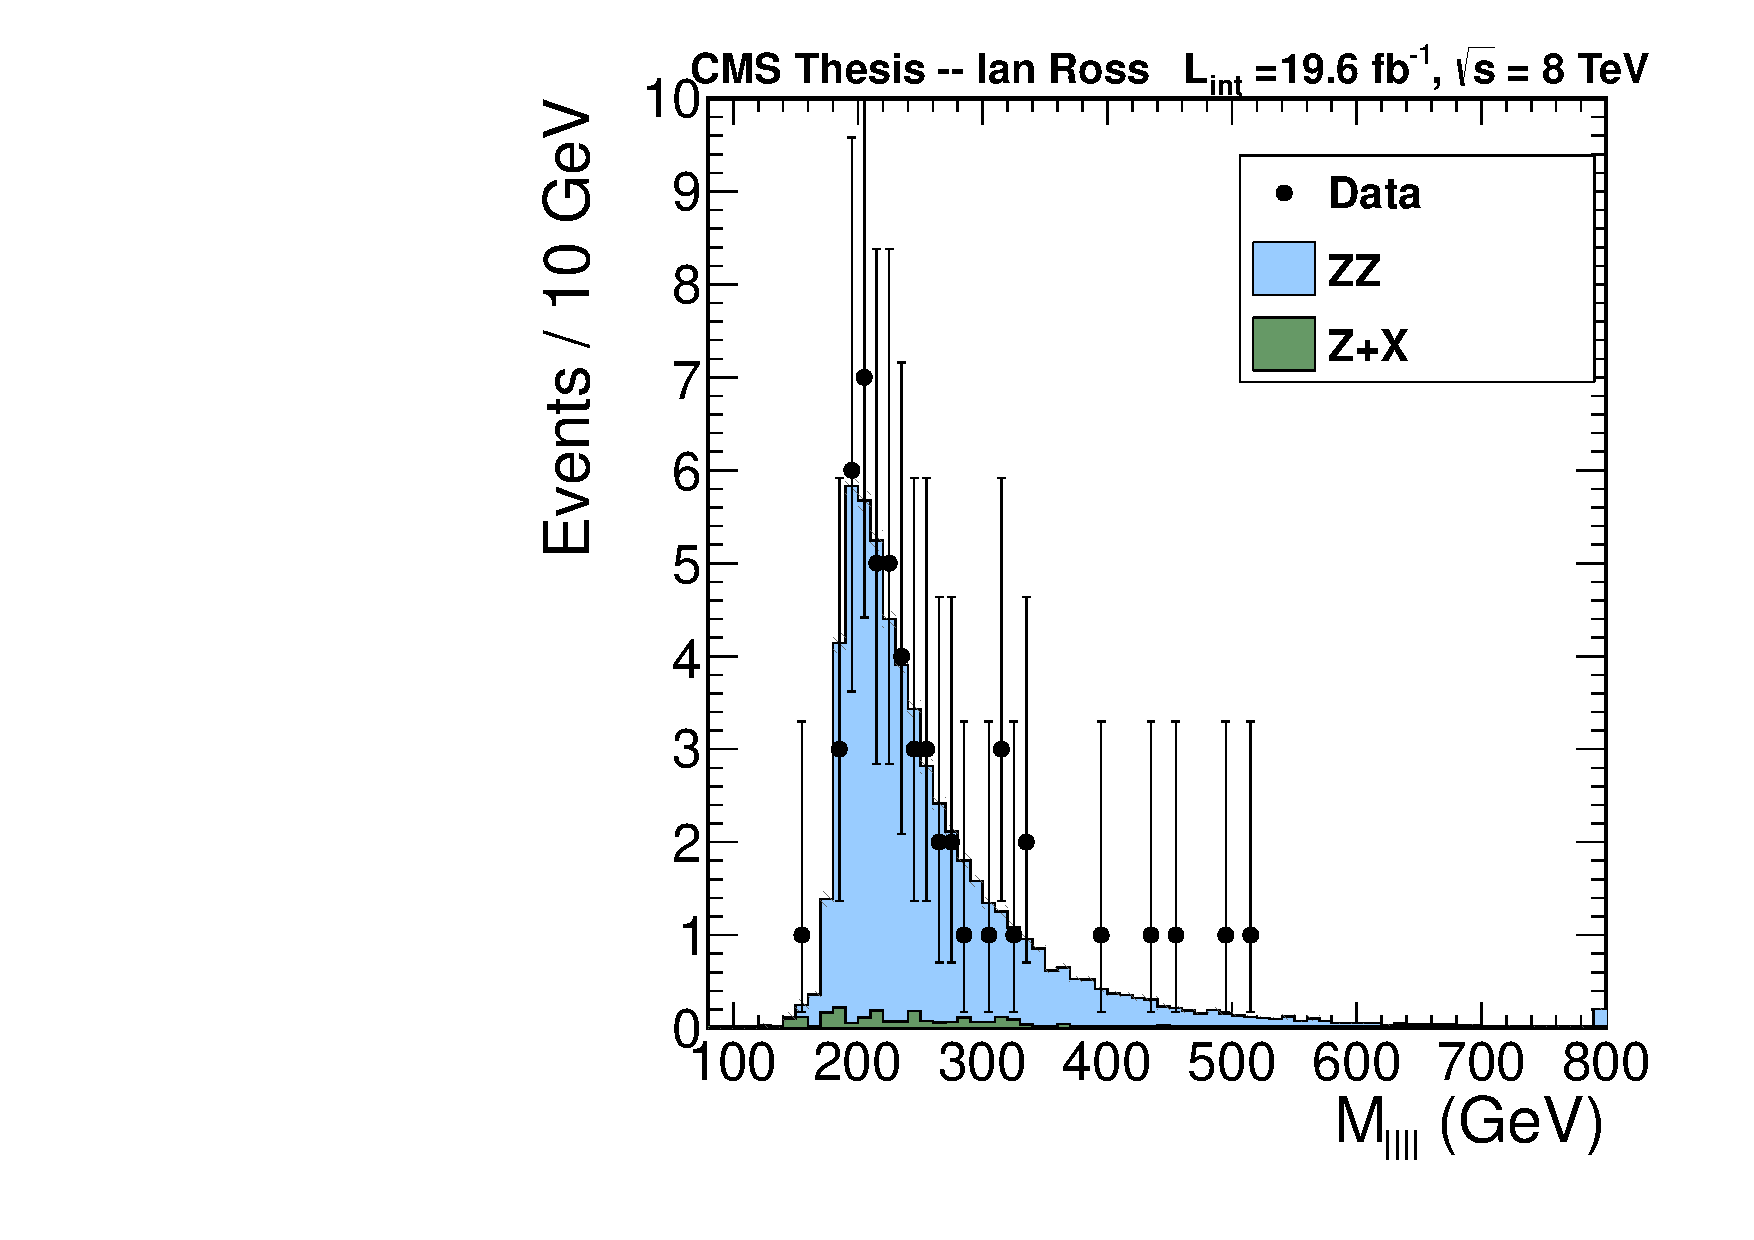
\includegraphics[width=0.40\textwidth]{eeee_mass_highmass}
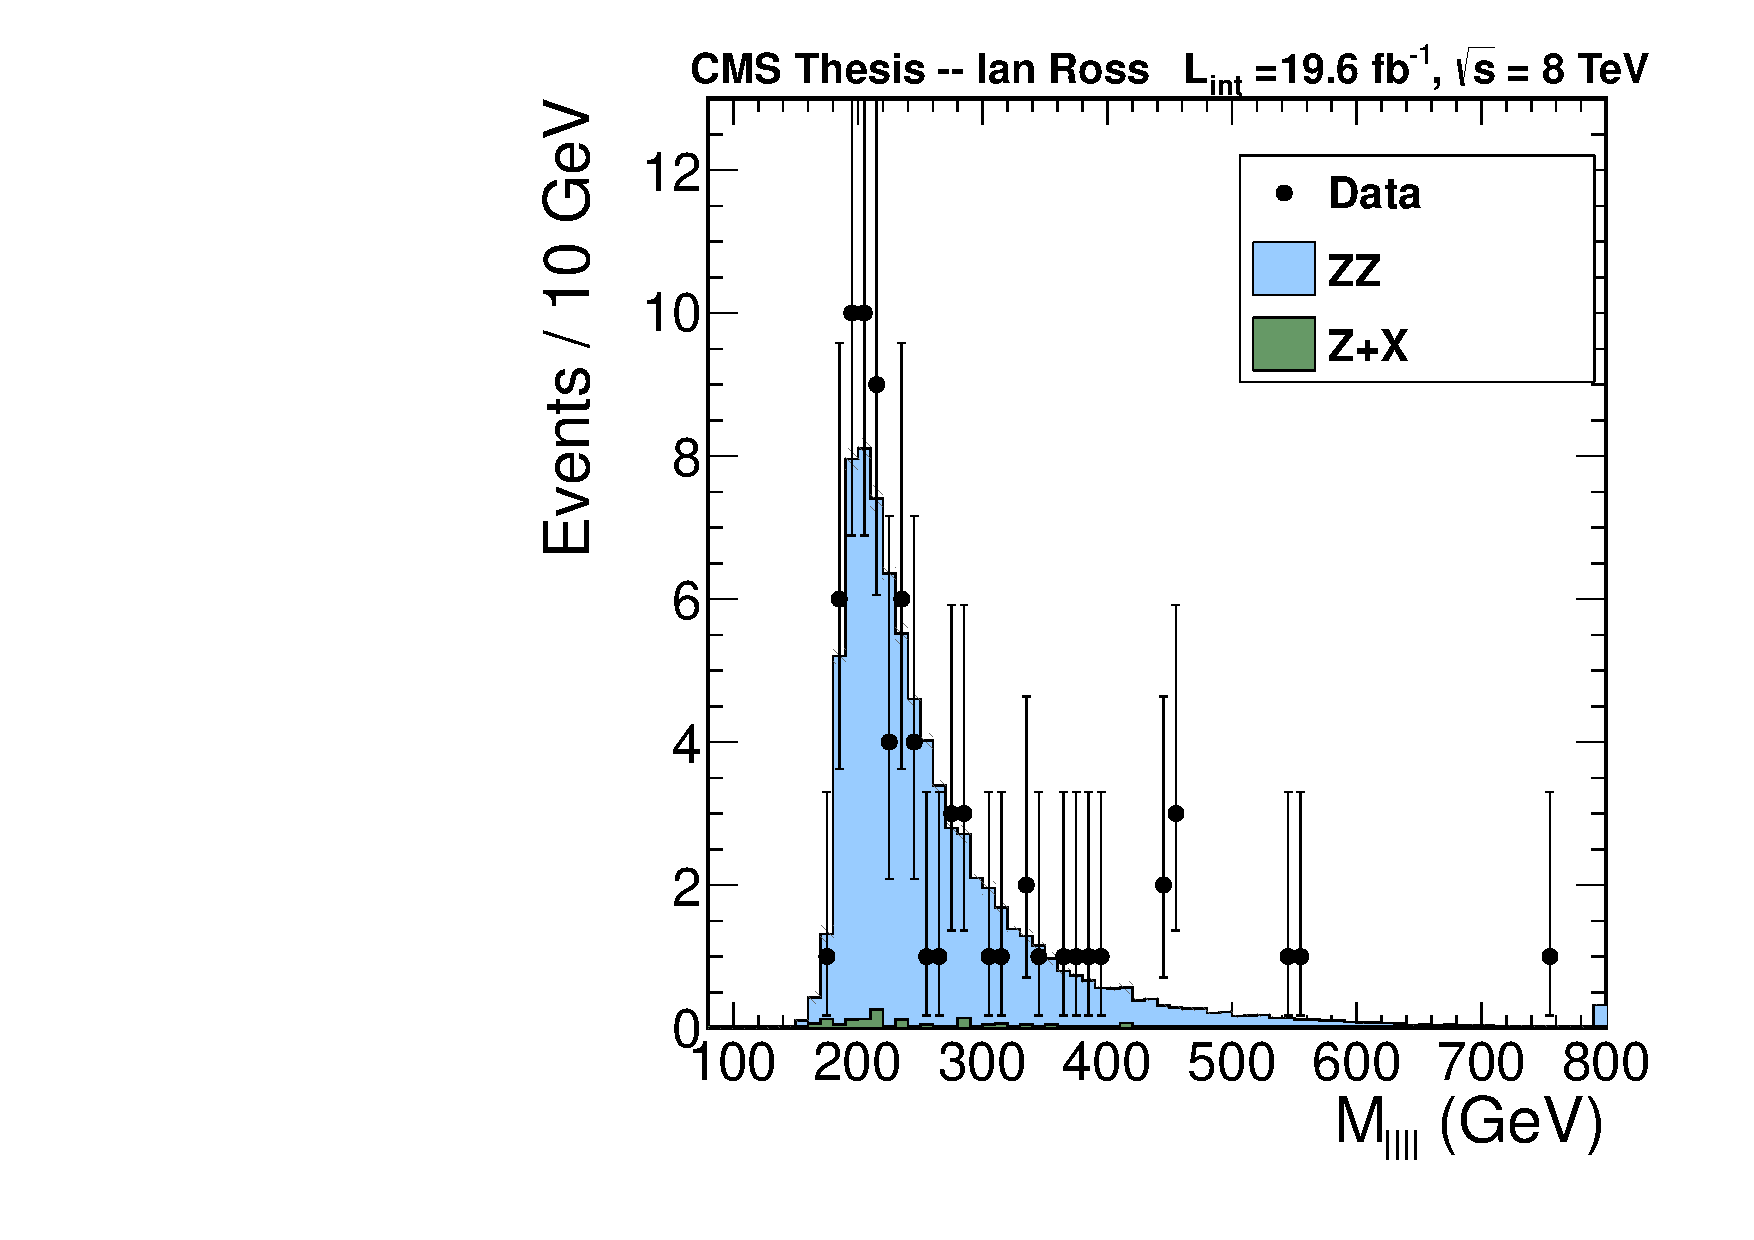
\includegraphics[width=0.40\textwidth]{mmmm_mass_highmass}\\
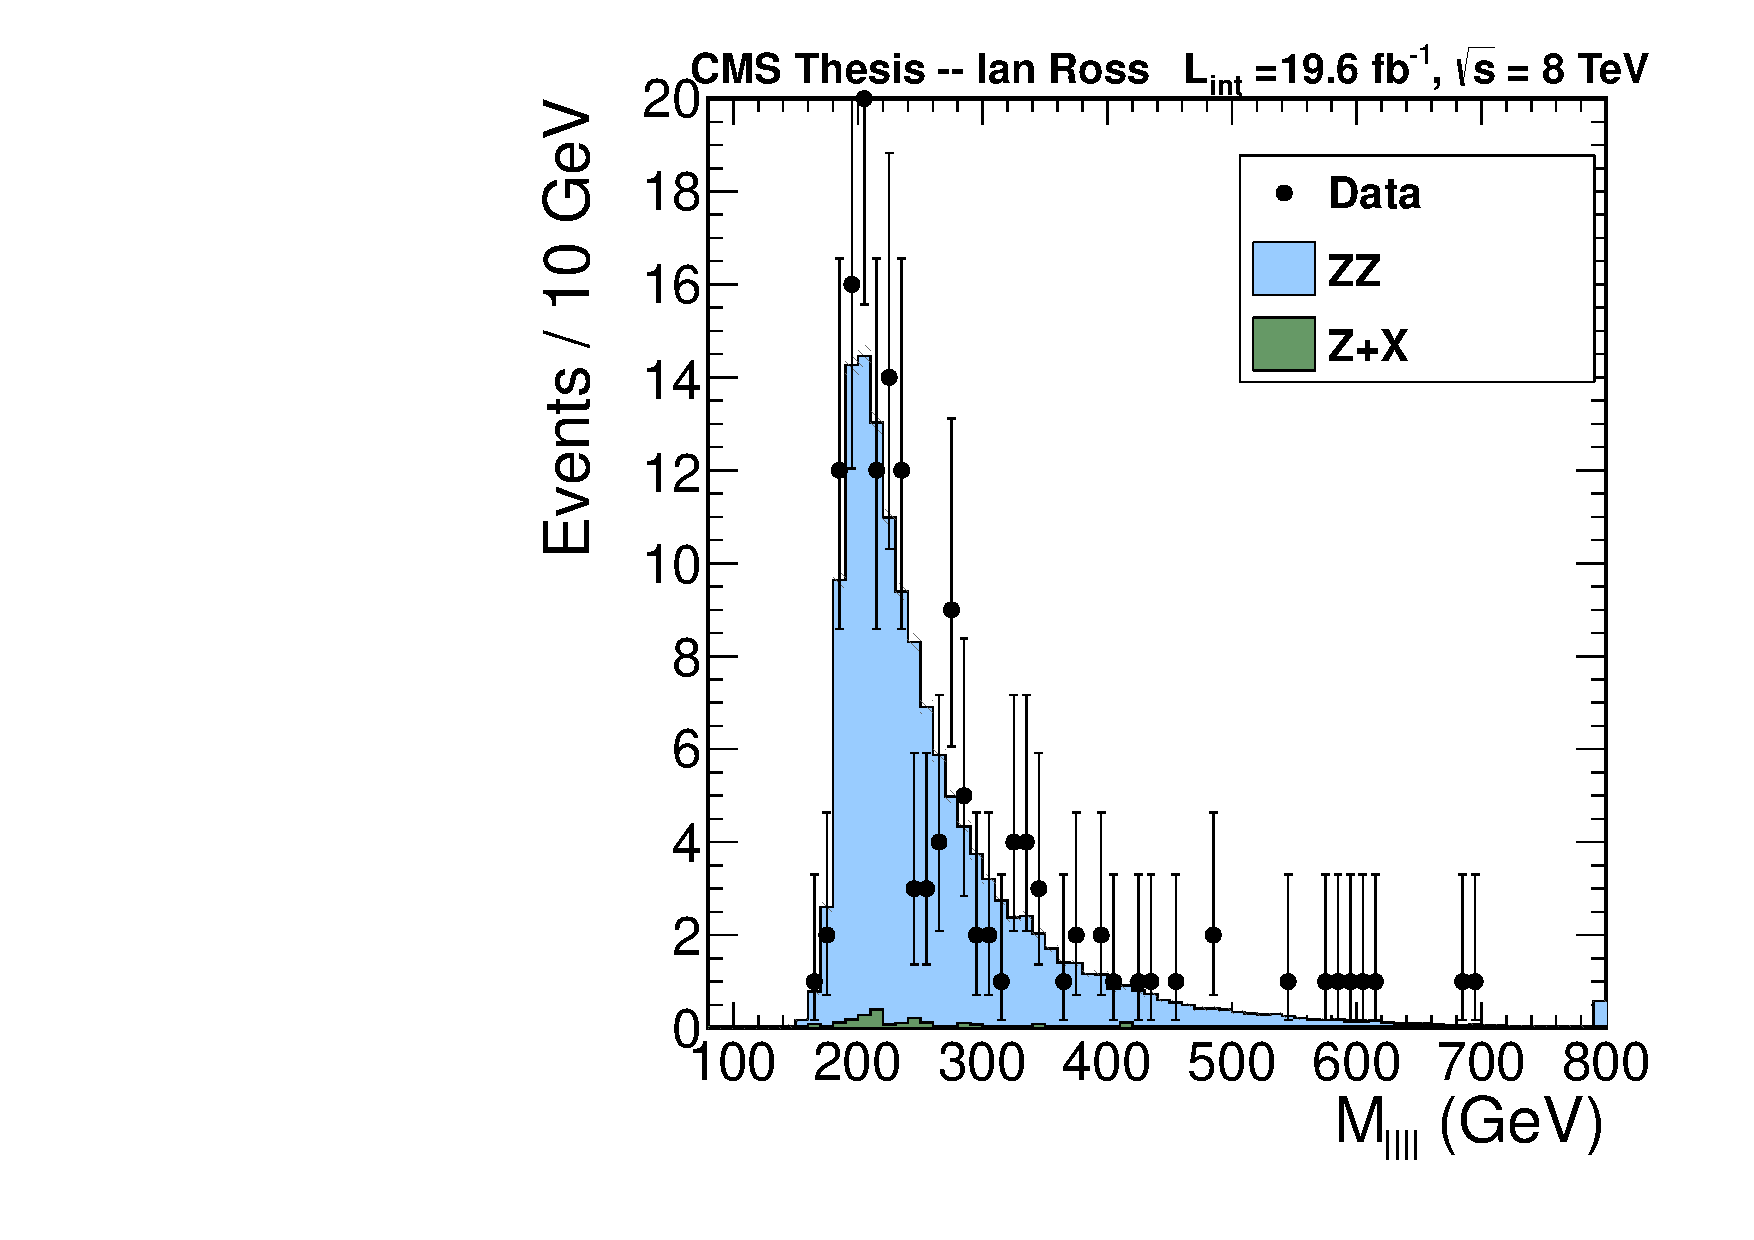
\includegraphics[width=0.40\textwidth]{eemm_mass_highmass}
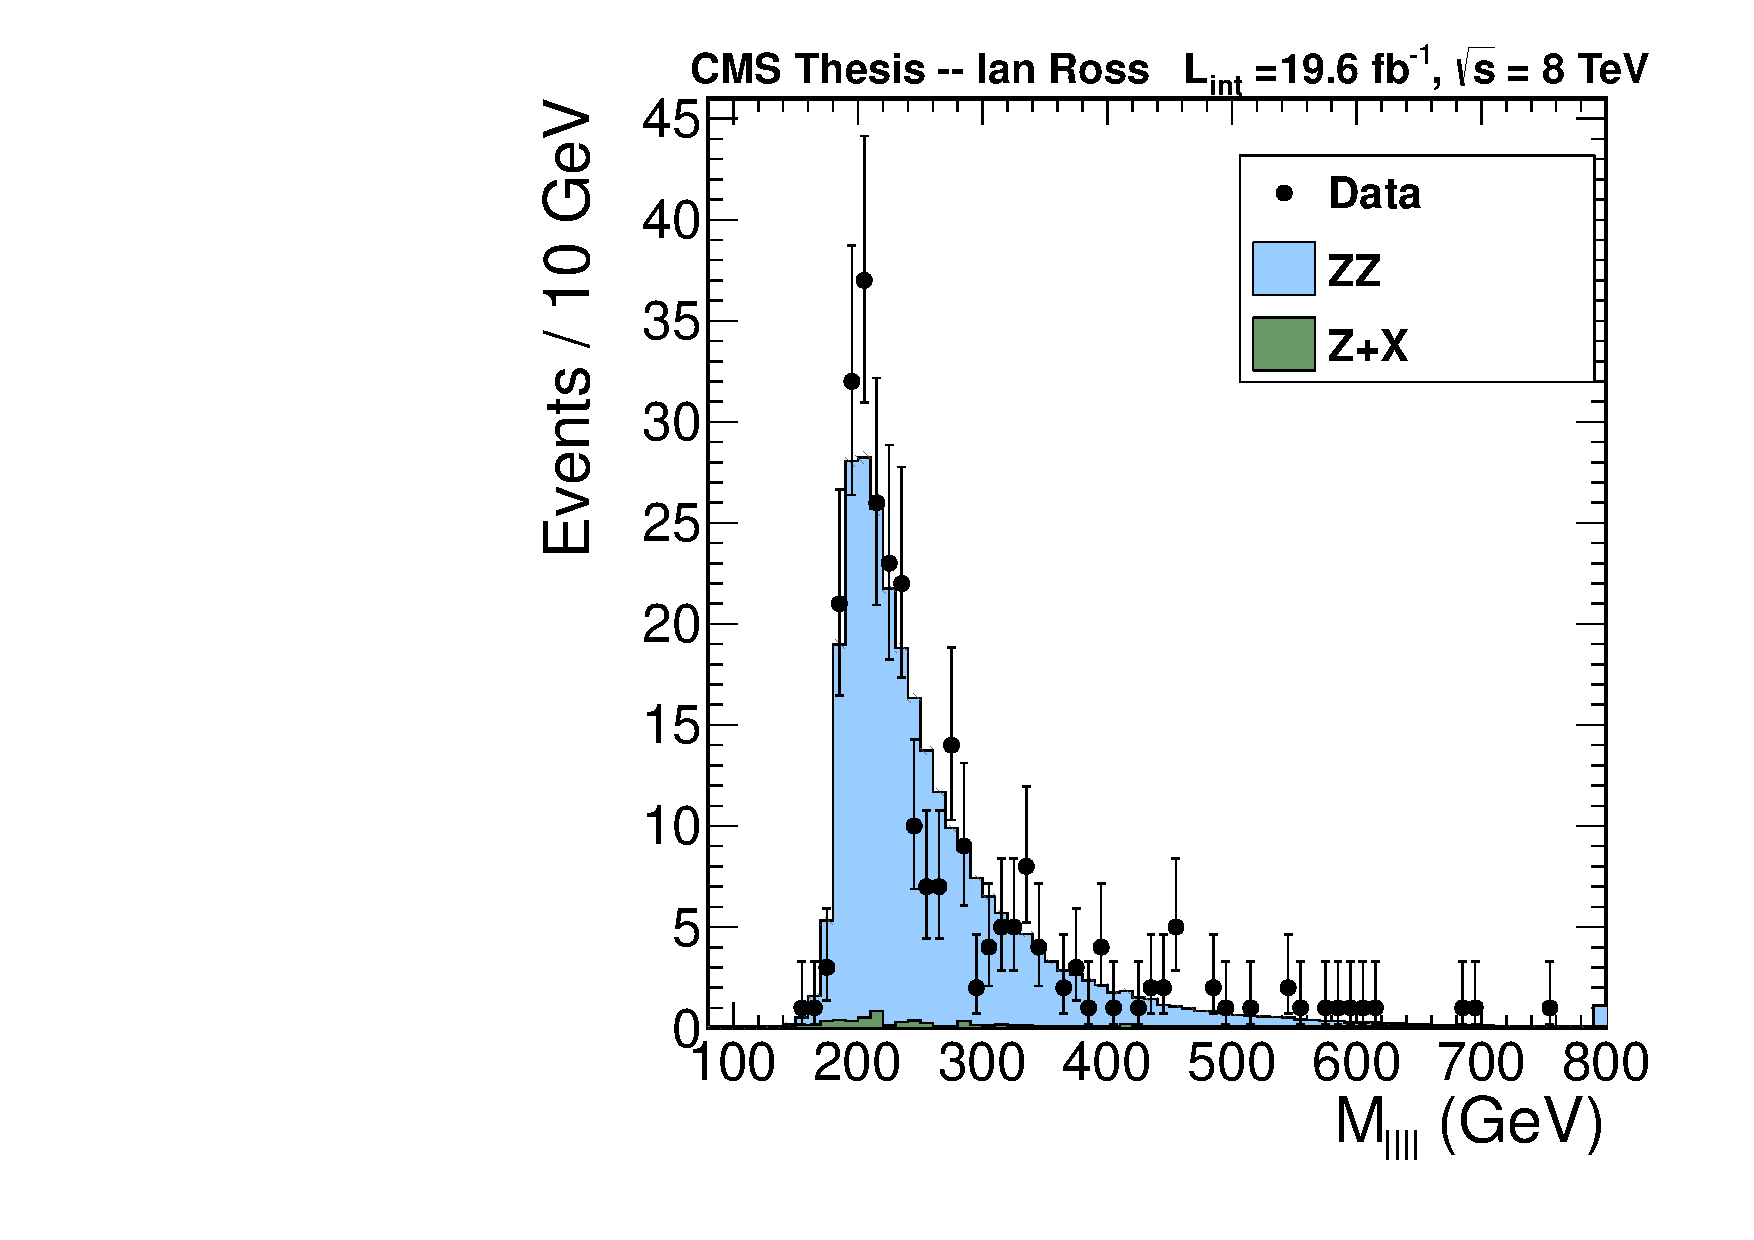
\includegraphics[width=0.40\textwidth]{4l_mass_highmass}
\caption[ZZ invariant mass for the high-mass analysis, across the full
considered $M_{\ell\ell\ell\ell}$ range.]{ZZ invariant mass for the high-mass
analysis, across the full considered $M_{\ell\ell\ell\ell}$ range. 
Pictured are
the eeee, $\mu\mu\mu\mu$, $\mu\mu e e$, and combined total results (upper left,
upper right, lower left, and lower right respectively).}
\label{fig:zzMass_high_full}
\end{figure}

\subsection{Cross section measurement} 
The first step of the statistical analysis is to define a likelihood function.
Because we are dealing with a counting experiment in each bin, the natural basis
to use is the Poisson distribution:
\begin{equation}
    f(k; \lambda) =\frac{\lambda^k e^{-k}}{k!} 
\end{equation}
Where $f(k; \lambda)$ is the probability of observing $k$ events, given an
expectation of $\lambda$. In the case of a physics search, k can be defined as:
\begin{equation}
    k = \mu s(\vec{\theta_s}) + b(\vec{\theta_b})
\end{equation}
where $\mu$ is a strength modifier (interpreted as
$\sigma_{measured}/\sigma_{SM}$) on the expected signal, $s$, and $b$ is the
expected background. $\vec{\theta_s}$ and $\vec{\theta_b}$ are the
nuisance parameters associated with the signal and background. These nuisance
parameters enter the expected yields as log-normal constraints.  The total
likelihood, then, is the product of the Poissonian distribution, across all bins
of the histogram:
\begin{equation}
    \label{eqn:likelihood}
    L(\mu, \vec{\theta_s}, \vec{\theta_b}) = \prod f_i(k_i; \lambda_i (\mu,
    \vec{\theta_s}, \vec{\theta_b}))
\end{equation}

The ZZ production cross section is extracted via a simultaneous fit to a likelihood
built from each of the final states. For the case of cross section extraction, a
global counting experiment is used (meaning there is just one bin considered in
Eqn.~\ref{eqn:likelihood} for each final state). 

By maximizing the likelihood function as a function of the signal strength
modifier, $\mu$, one can extract the measured cross section. After removing the
branching ratio of the Z decays into leptons, the ZZ production cross section is
measured as:
\begin{equation}
    \sigma(pp\rightarrow ZZ) = 7.7^{+0.5}_{-0.5} \textrm(stat.) ^{+0.6}_{-0.5}
    \textrm{(sys.)}  \pm 0.3 \textrm{(lumi)} \textrm{pb}
\end{equation}
which agrees favorably with the Standard Model prediction (from MCFM~\cite{MCFM})
of $7.7 \pm 0.6$ pb.
The cross section is also measured using each channel individually. These
results are shown in table~\ref{tab:cross_sections}.

\begin{table}[h]
\centering
\begin{tabular}{|c|c|}
\hline
Final State & $ \sigma(pp \rightarrow ZZ) $ \\
\hline
$\mu\mu\mu\mu$ & 
$    7.3^{+0.8}_{-0.8} \textrm(stat.) ^{+0.7}_{-0.6}
\textrm{(sys.)}  \pm 0.3 \textrm{(lumi)} \textrm{pb} $\\
 eeee & 
    $7.2^{+1.0}_{-0.9} \textrm(stat.) ^{+0.7}_{-0.6}
\textrm{(sys.)}  \pm 0.3 \textrm{(lumi)} \textrm{pb} $\\

$ \mu \mu ee$ & 
    $8.1^{+0.7}_{-0.6} \textrm(stat.) ^{+0.7}_{-0.6}
\textrm{(sys.)}  \pm 0.4 \textrm{(lumi)} \textrm{pb} $\\
Combined & 
    $7.7^{+0.5}_{-0.5} \textrm(stat.) ^{+0.6}_{-0.5}
\textrm{(sys.)}  \pm 0.3 \textrm{(lumi)} \textrm{pb} $\\
\hline
\end{tabular}
\caption[ZZ production cross section measurements for each of the final states
considered and combined.]{ZZ production cross section measurements for each of the final states
considered and combined.}
\label{tab:cross_sections}
\end{table}

\subsection{Unfolding}
In order to remove detector effects from the differential cross sections, the
distributions are \emph{unfolded}. The procedure followed within this analysis
is the iterative Bayesian method, outlined by D'Agostini~\cite{unfolding}.

The measured distribution of a variable is assumed to be a convolved mixture of
the underlying ``true'' distribution and the smearing and distortion resulting
by imperfect detector elements. Specifically, the measured distribution, M, is
related to the true distribution T, through a response matrix, R:
\begin{equation}
    M_i = \sum\limits_j R_{ij} T_j
\end{equation}
The response matrix, $R$, is trained with a Monte Carlo sample,
passing the generated and reconstructed values from each event
into the corresponding (true value, reconstructed value) bin. 
Bayes' theorem is then applied to the elements, using a flat prior, to give the
probability of a true value from bin $i$, given an observation in bin $j$:
\begin{equation}
    P(T_i | M_j) = \frac{P(M_j | T_I) P_0(T_i)}{\sum\limits_{l=1}^{nbins truth}
    P(M_j | T_l) P_0(T_l)}
\end{equation}
And the estimate for the number of true events in bin $i$, is
\begin{equation}
    n_i = \frac{1}{\epsilon_i} \sum\limits_{j=1}^{nbins reco} n_j P(T_i |
    M_J)
\end{equation}
where $\epsilon_i$ is the overall efficiency for reconstructing an event originating
in bin i and $n_j$ is the total number of events observed in bin $j$.
The prior probability, $P_0$ is initially assumed to be flat. However, an
iterative process is used while training, recursively updating the prior until
the predicted and actual true distributions match reasonably well. 

\begin{figure}[h]
\centering
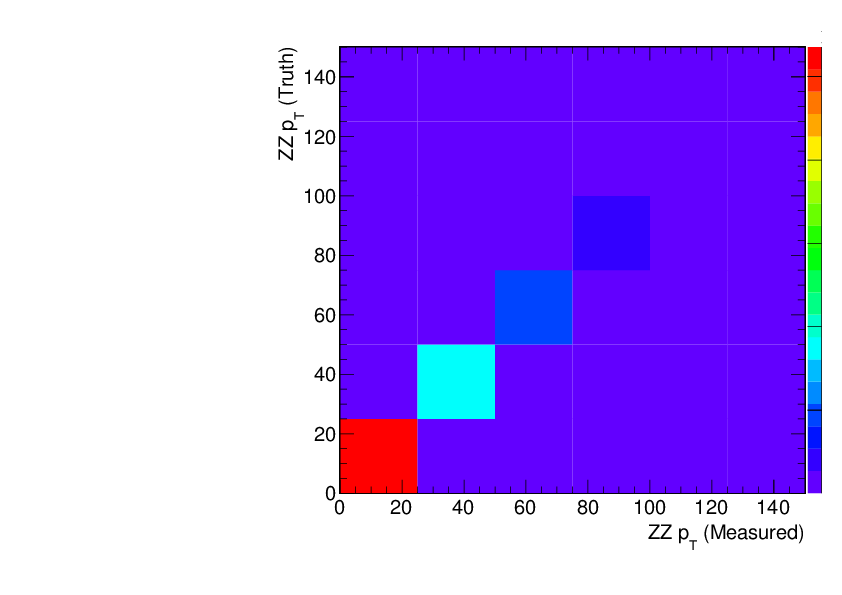
\includegraphics[width=0.45\textwidth]{llll_pt_responseMat}
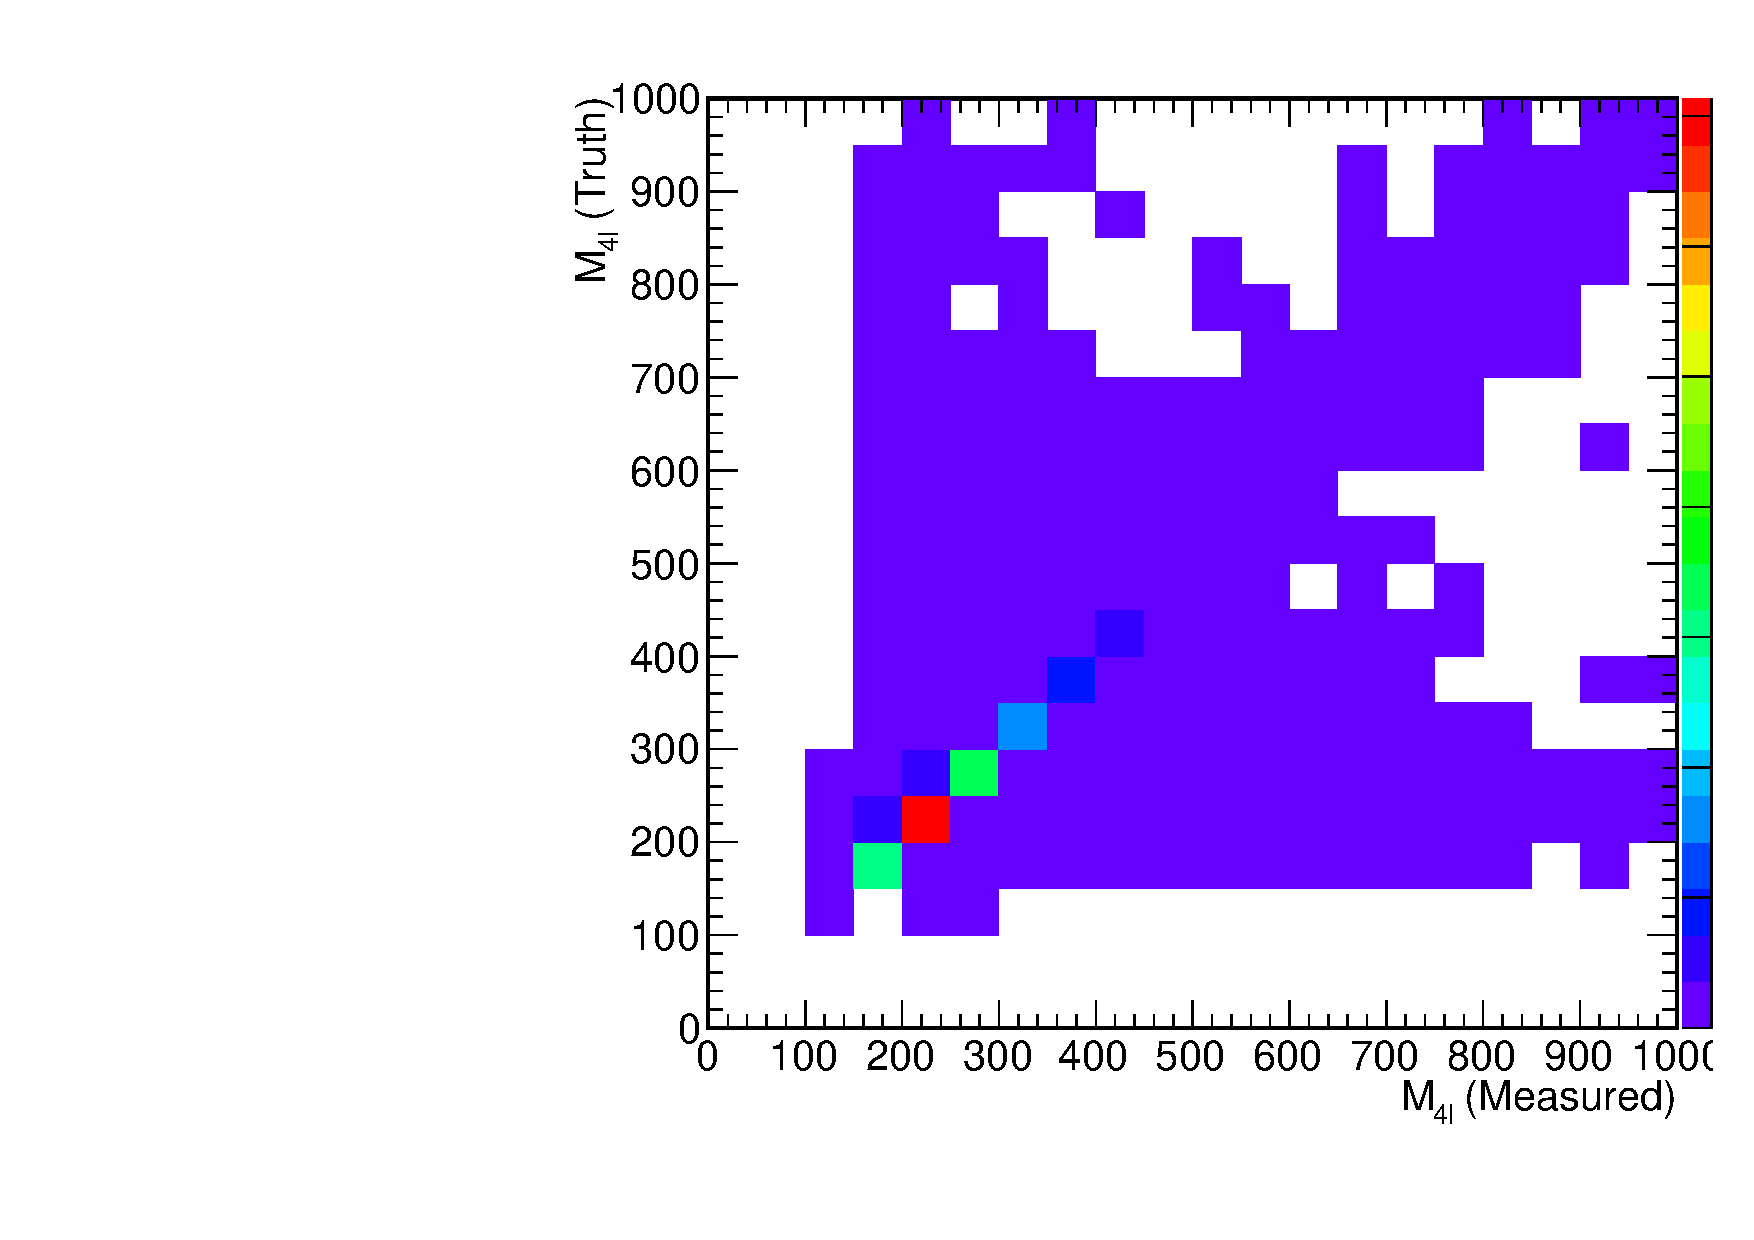
\includegraphics[width=0.45\textwidth]{llll_mass_responseMat} \\
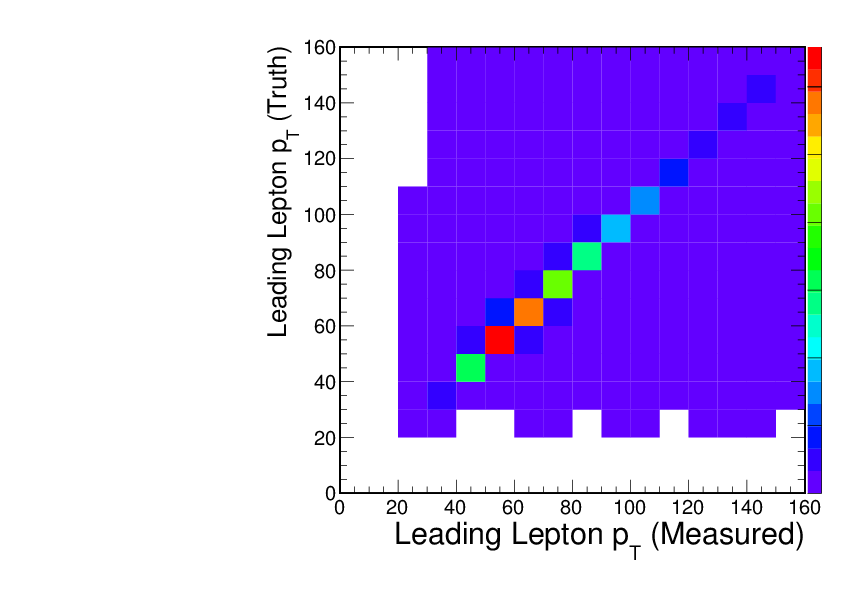
\includegraphics[width=0.45\textwidth]{leadingLep_pt_responseMat}
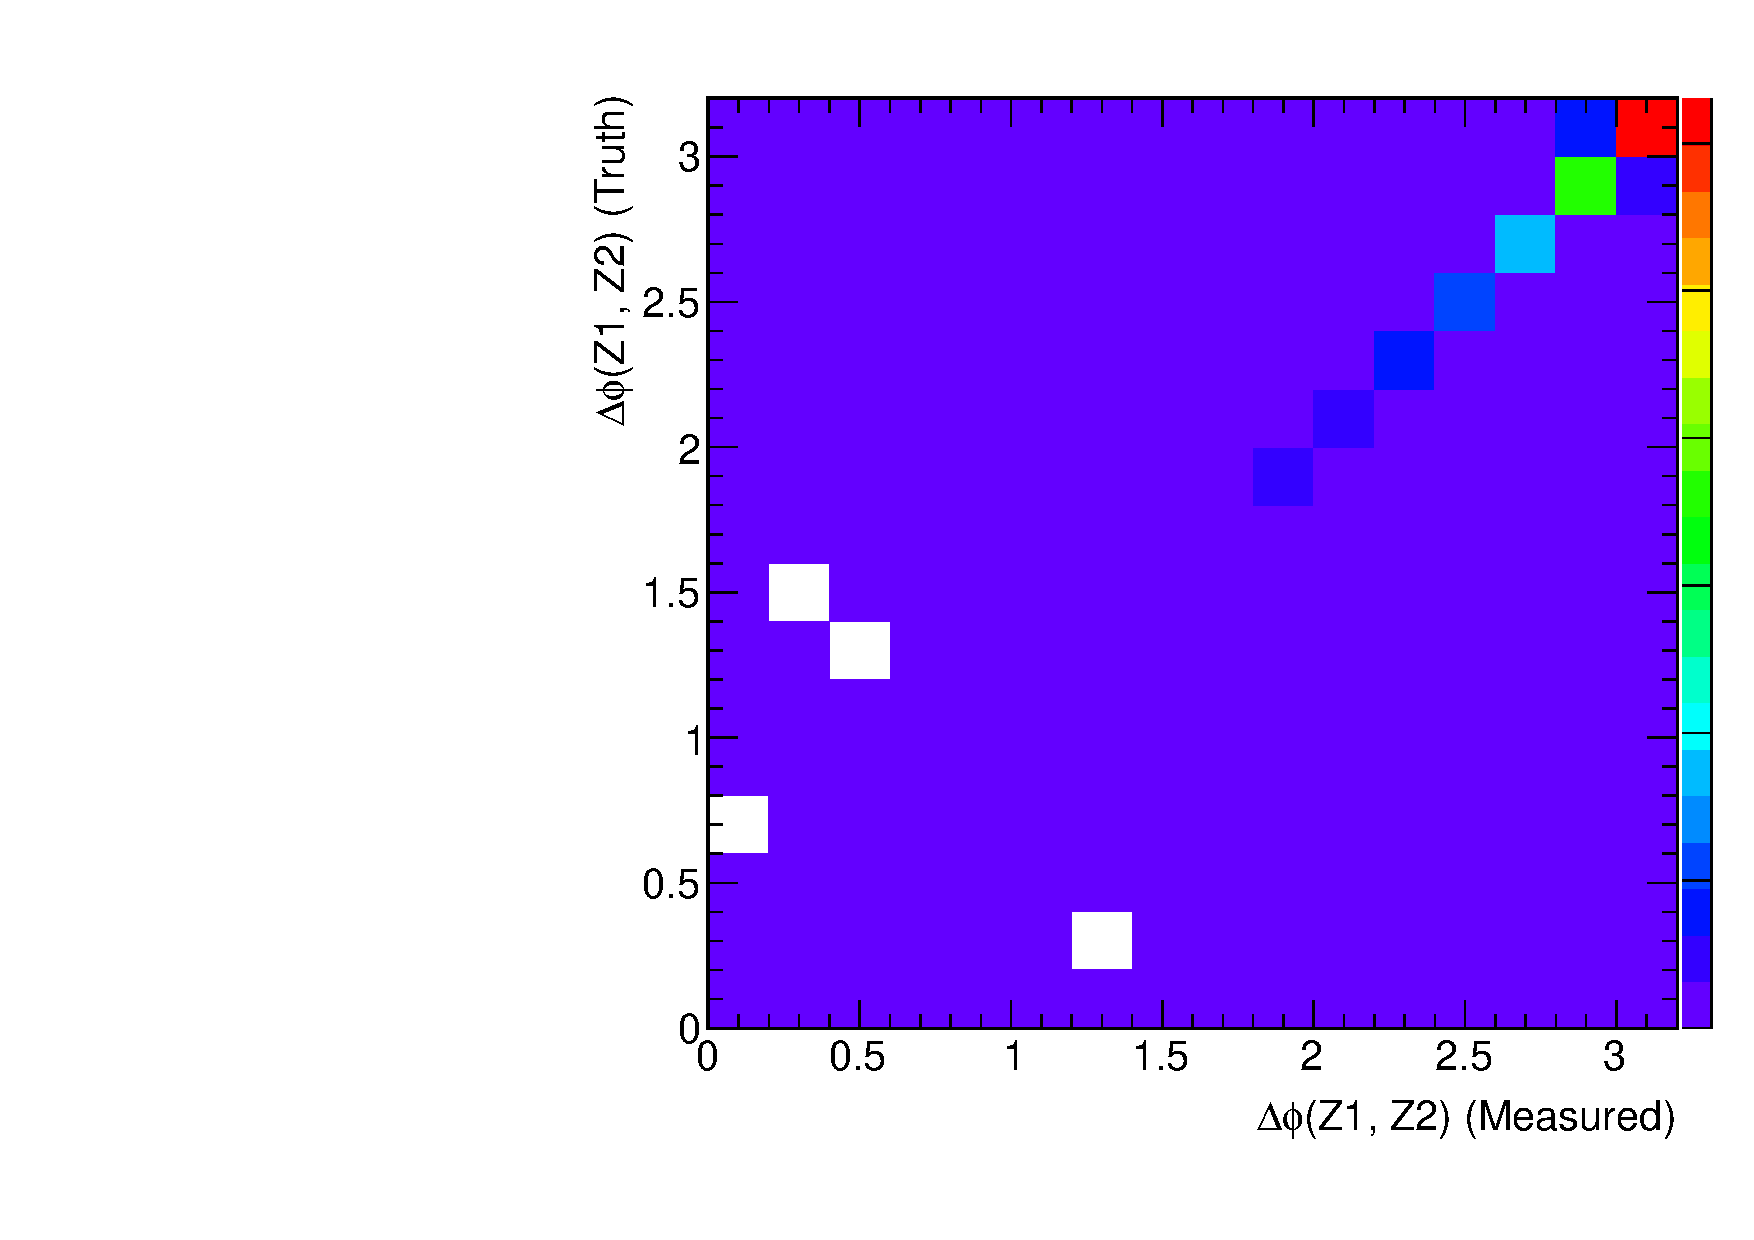
\includegraphics[width=0.45\textwidth]{dPhi_Zs_responseMat}
\caption[Example response matrices used in unfolding.]{Example response
matrices used in the unfolding process. Pictured, clockwise from the top left,
are the four-lepton $p_T$, four-lepton mass, leading lepton $p_T$, and azimuthal
separation between the Z bosons. The primarily diagonal nature indicates a
limited number of migrations, due to the excellent detector resolutions.}
\label{fig:responseMatrices}
\end{figure}

The CMS detector has, on the whole, excellent electron and muon
resolution, and as a result there is a limited amount of bin-to-bin migration.
A qualitative example of the unfolded vs. uncorrected distributions are shown in
figure~\ref{fig:unfoldedExample}.
Migrations between bins are slight overall, as are the resulting effects of the
unfolding.
This suggests that the overall detector resolution is excellent, in both
position and momenta measurements, for the objects utilized in the analysis.
Final unfolded differential distributions are presented in
Figures~\ref{fig:unfolding_leadingLepPt},~\ref{fig:unfolding_ZZ},~\ref{fig:unfolding_Z1},and
\ref{fig:unfolding_Z_separation}.

%\begin{figure}[h]
%\centering
%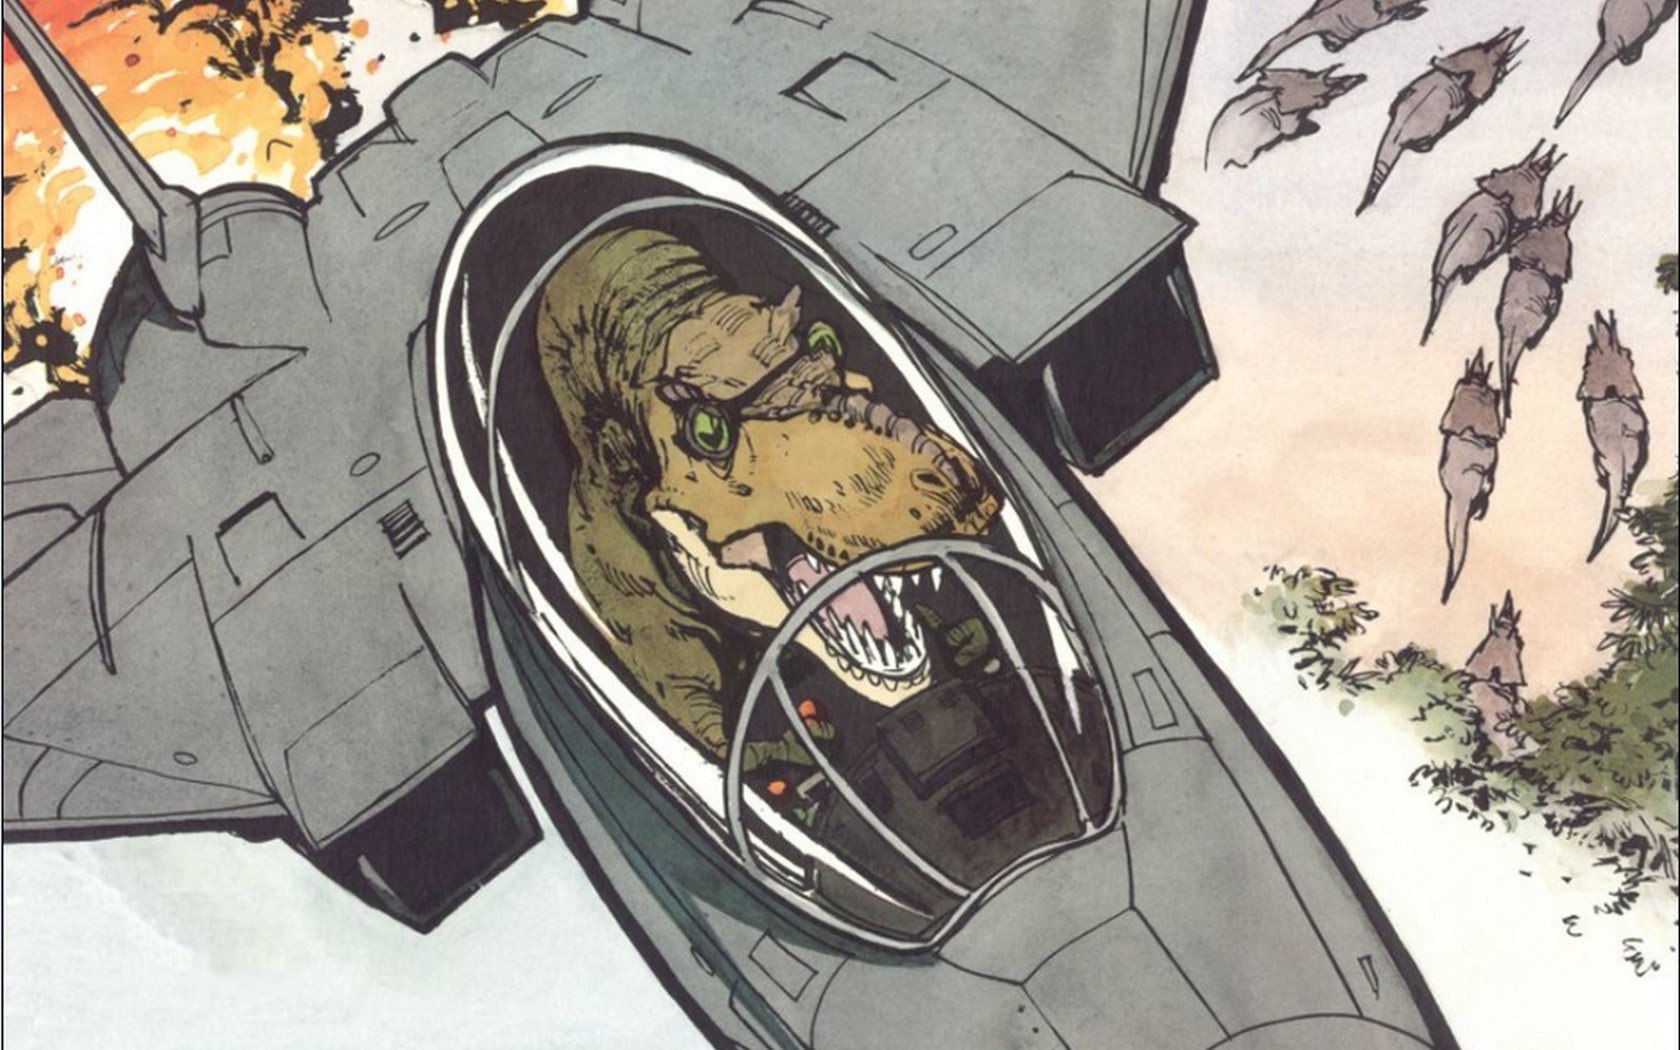
\includegraphics[width=0.40\textwidth]{placeholder}
%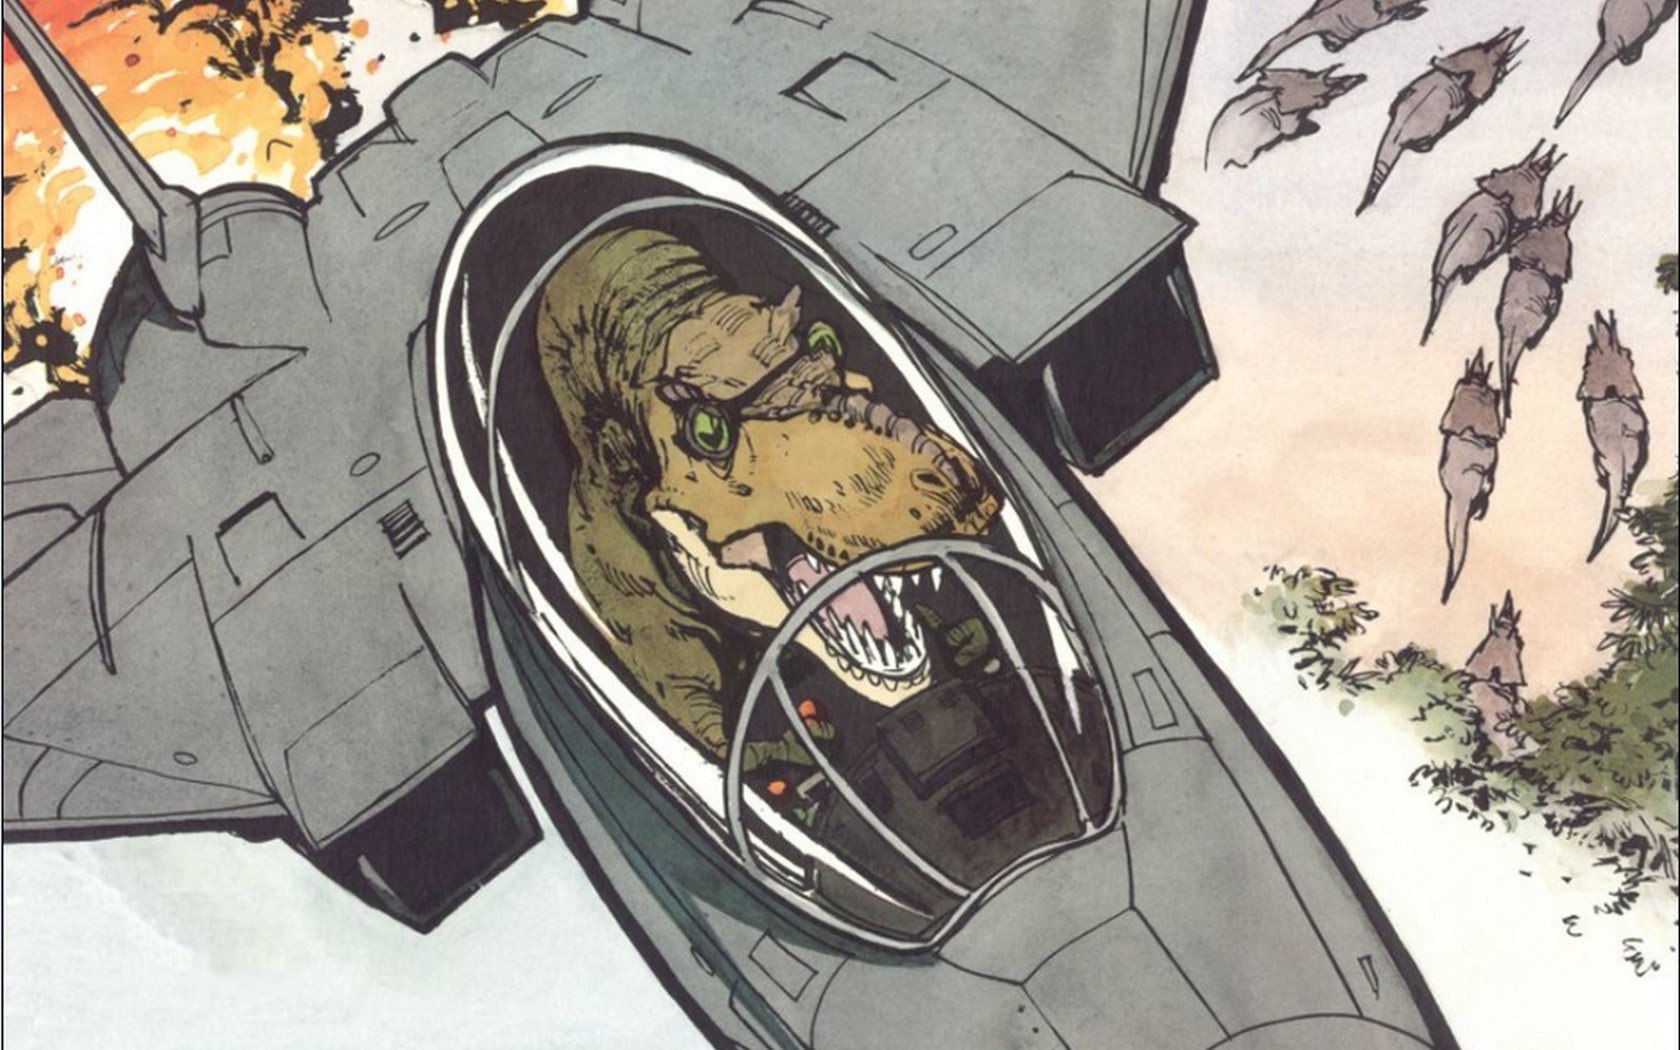
\includegraphics[width=0.40\textwidth]{placeholder} \\ 
%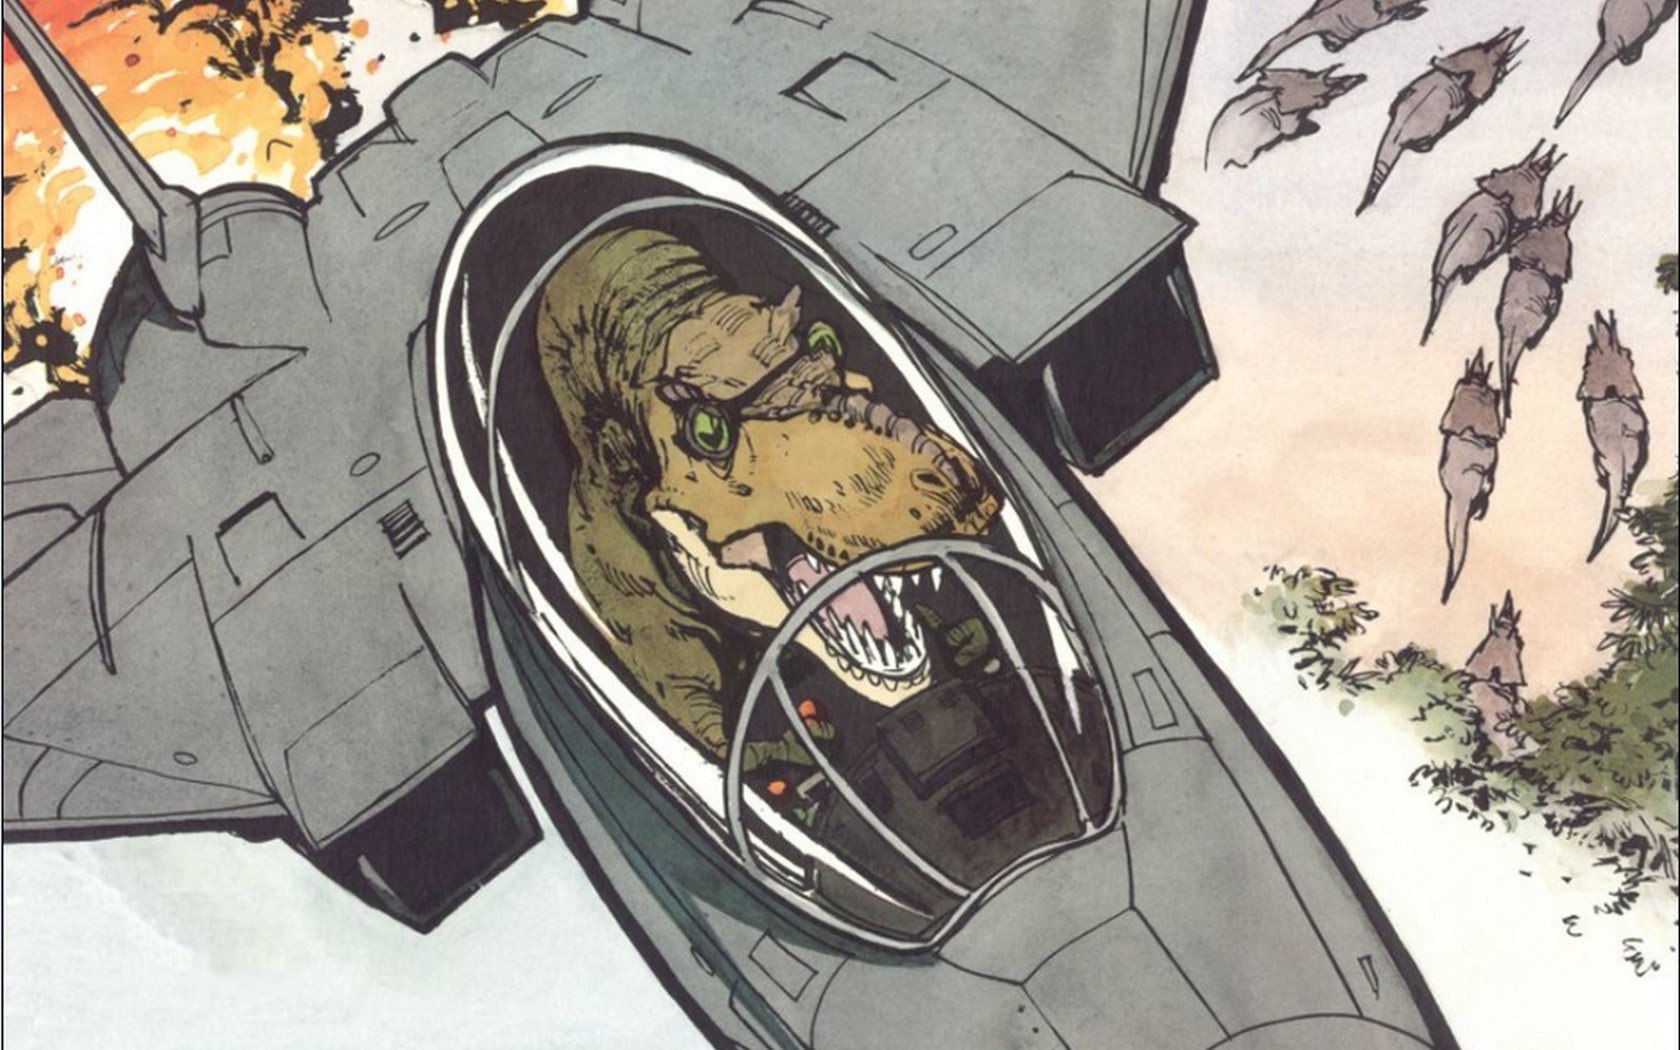
\includegraphics[width=0.40\textwidth]{placeholder}
%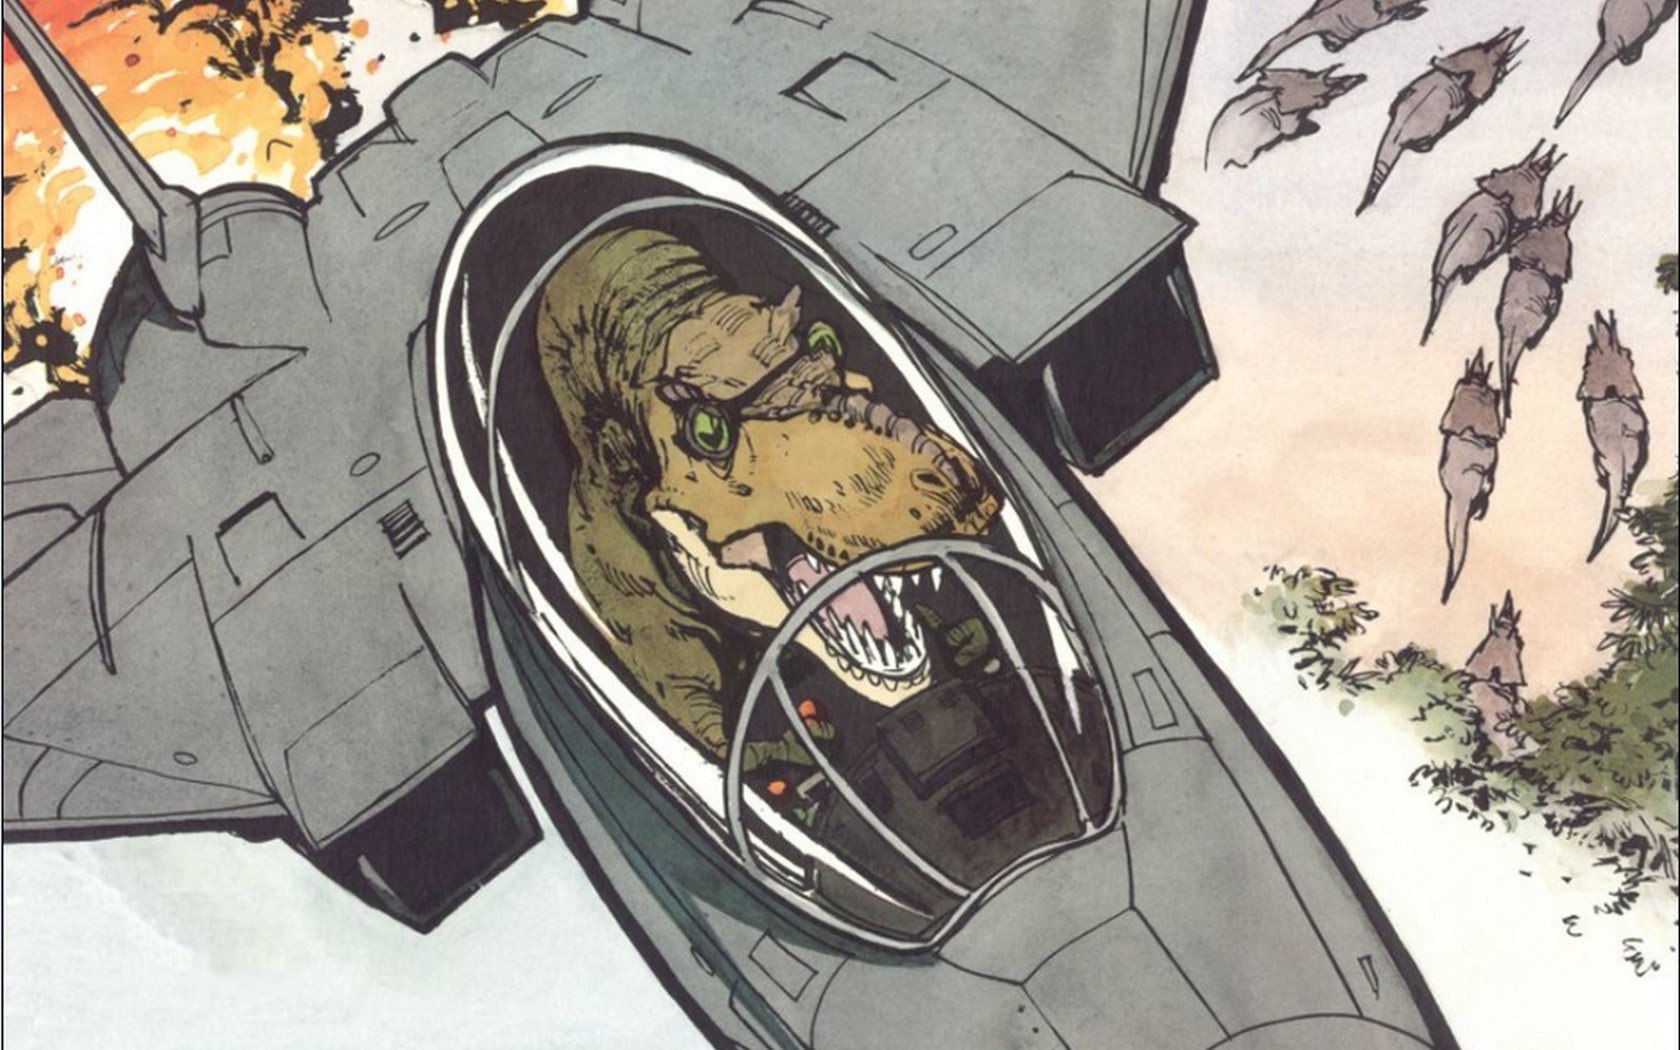
\includegraphics[width=0.40\textwidth]{placeholder} \\ 
%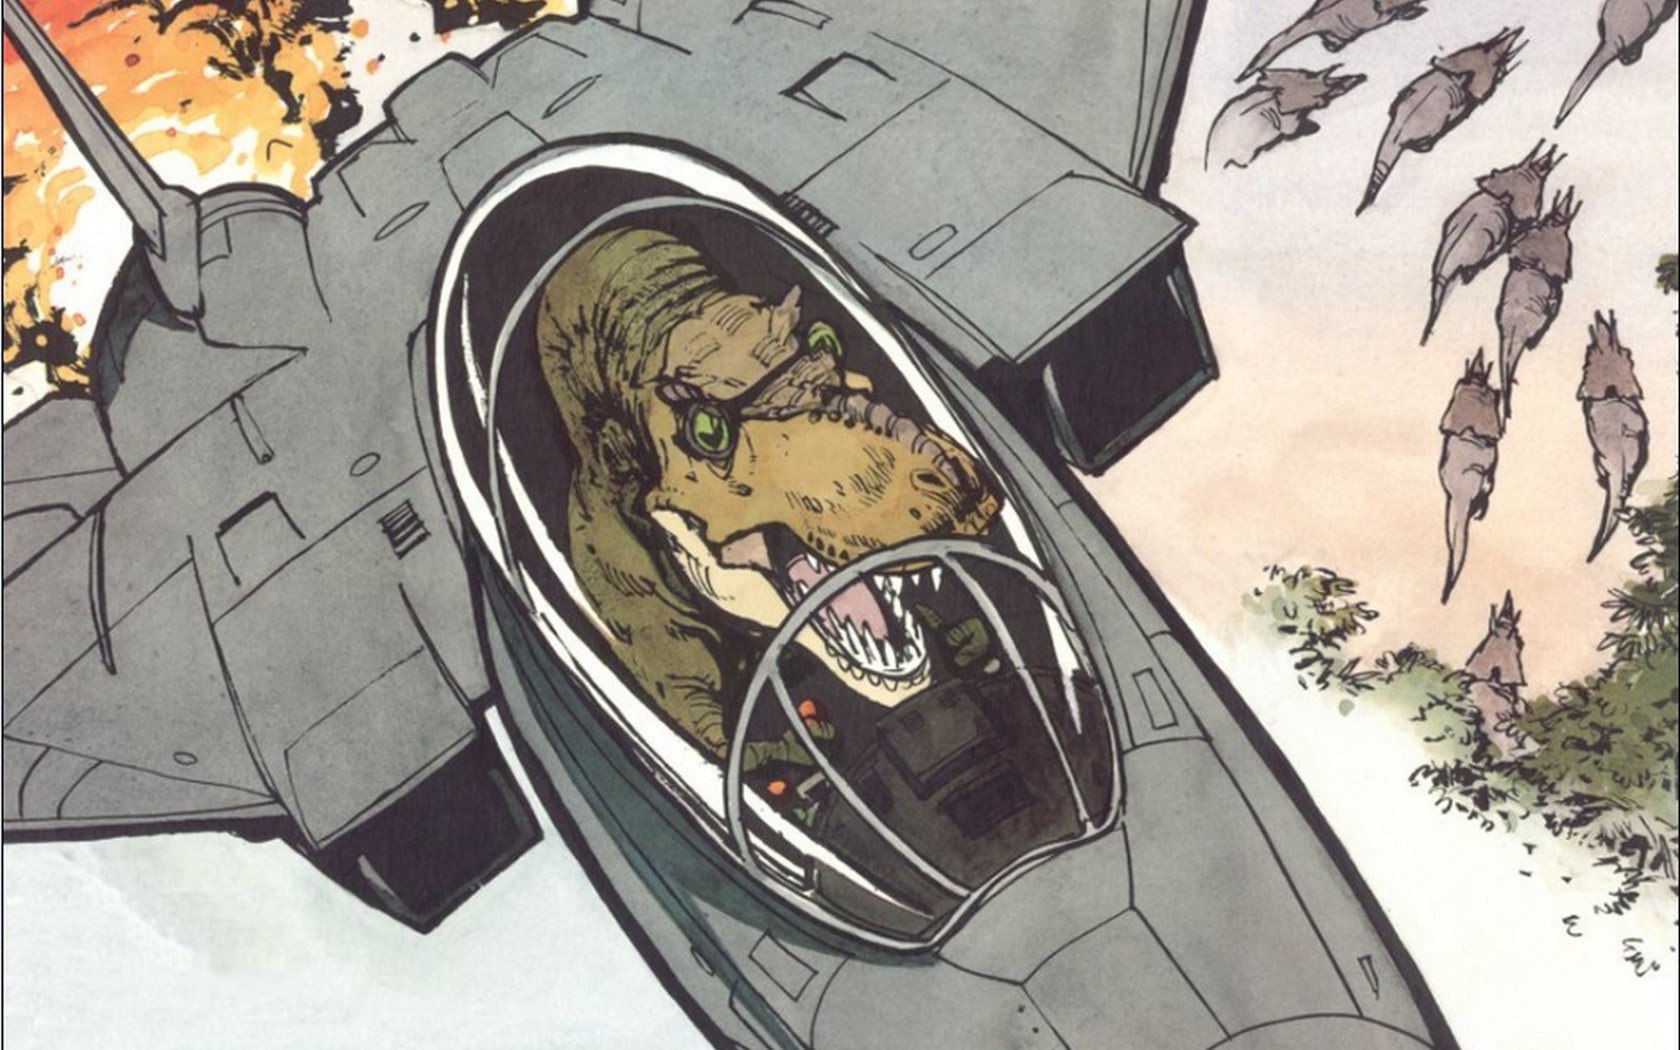
\includegraphics[width=0.40\textwidth]{placeholder}
%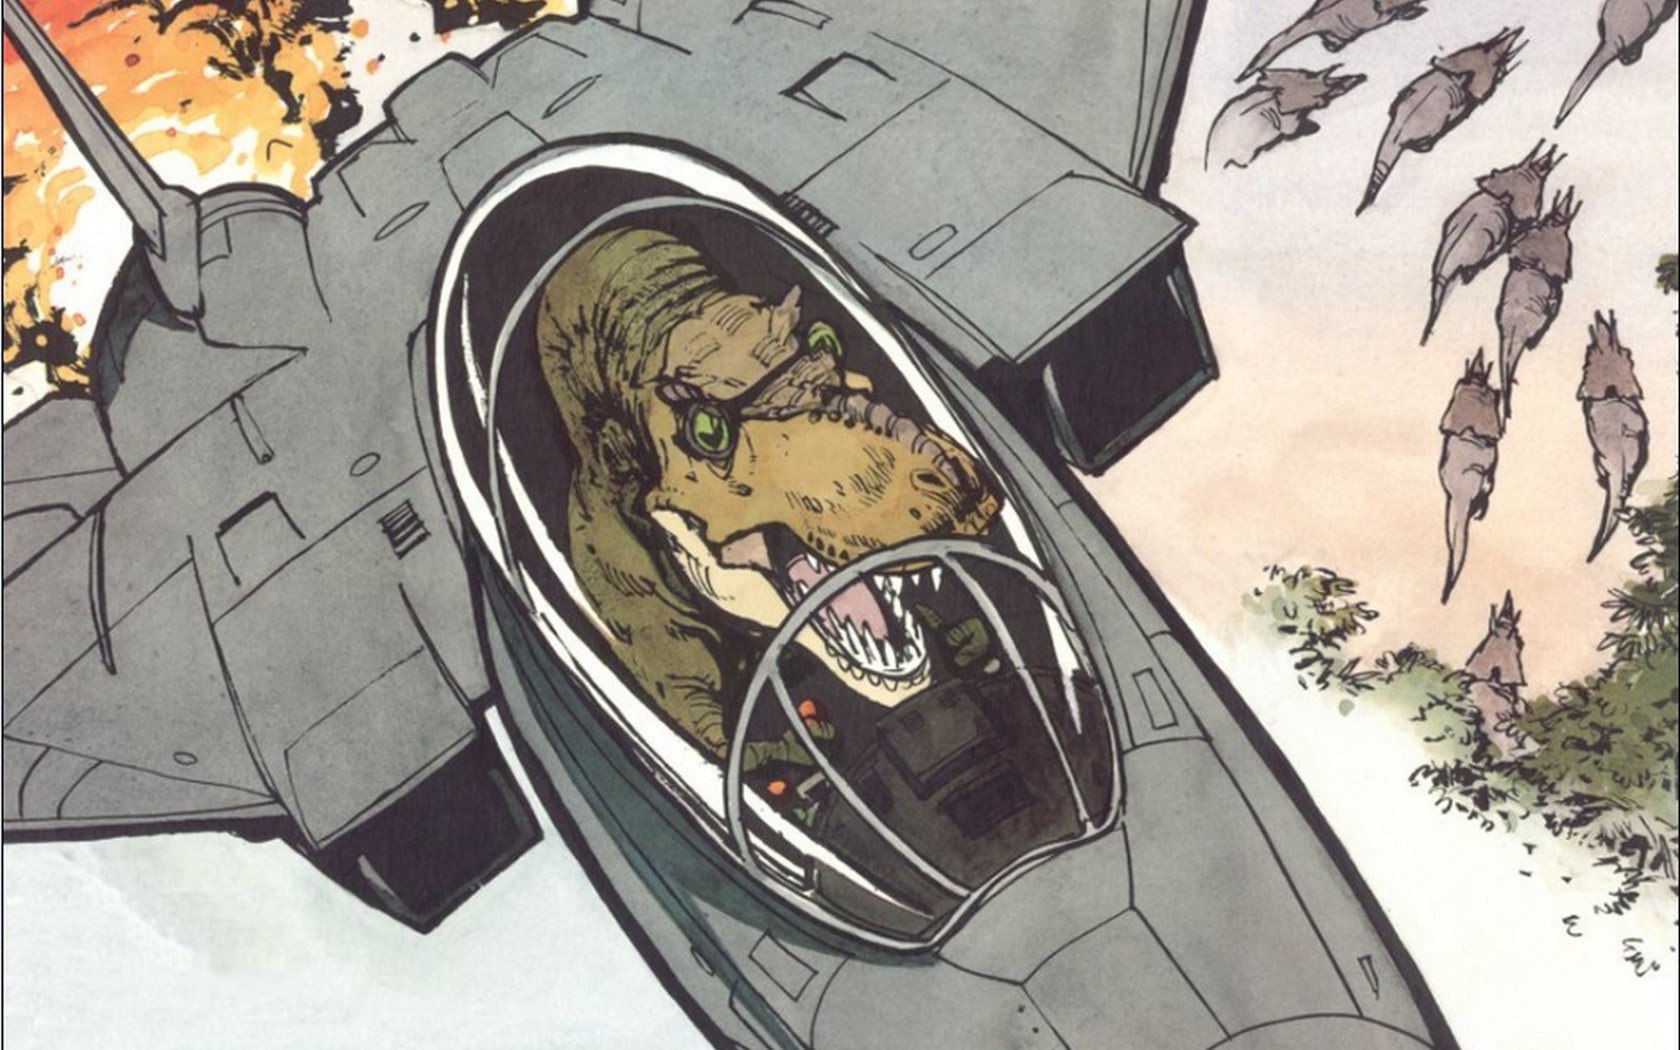
\includegraphics[width=0.40\textwidth]{placeholder} 
%\caption[Measured electron and muon resolutions (with comparison to generated
%resolutions).]{Measured electron and muon resolutions, with comparisons to
%generated resolutions. Muons (left) and electrons (right) both show excellent
%detector response in $p_{T}, \eta, \textrm{and} \phi$ (top, middle, and bottom
%respectively).}
%\label{fig:objectResolution}
%\end{figure}

\begin{figure}[h]
\centering
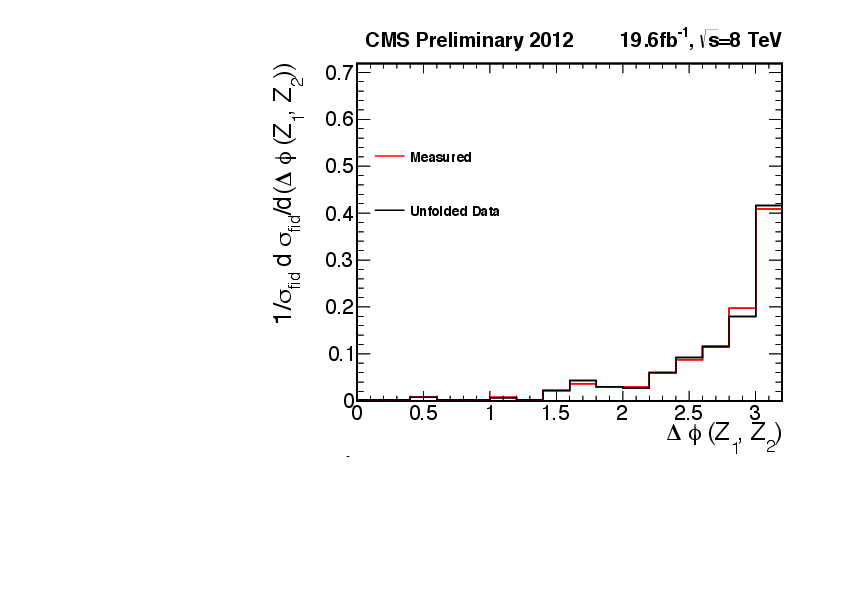
\includegraphics[width=0.80\textwidth]{dPhi_Zs_comp}
\caption[An example of the effects of unfolding.]{An example of the effects of
    unfolding. The $\Delta \phi$ separation between Z candidates is relatively
    unchanged by the unfolding (red, measured, and black, unfolded, are nearly
    identical).}
\label{fig:unfoldedExample}
\end{figure}
%%%%

\begin{figure}[h]
\centering
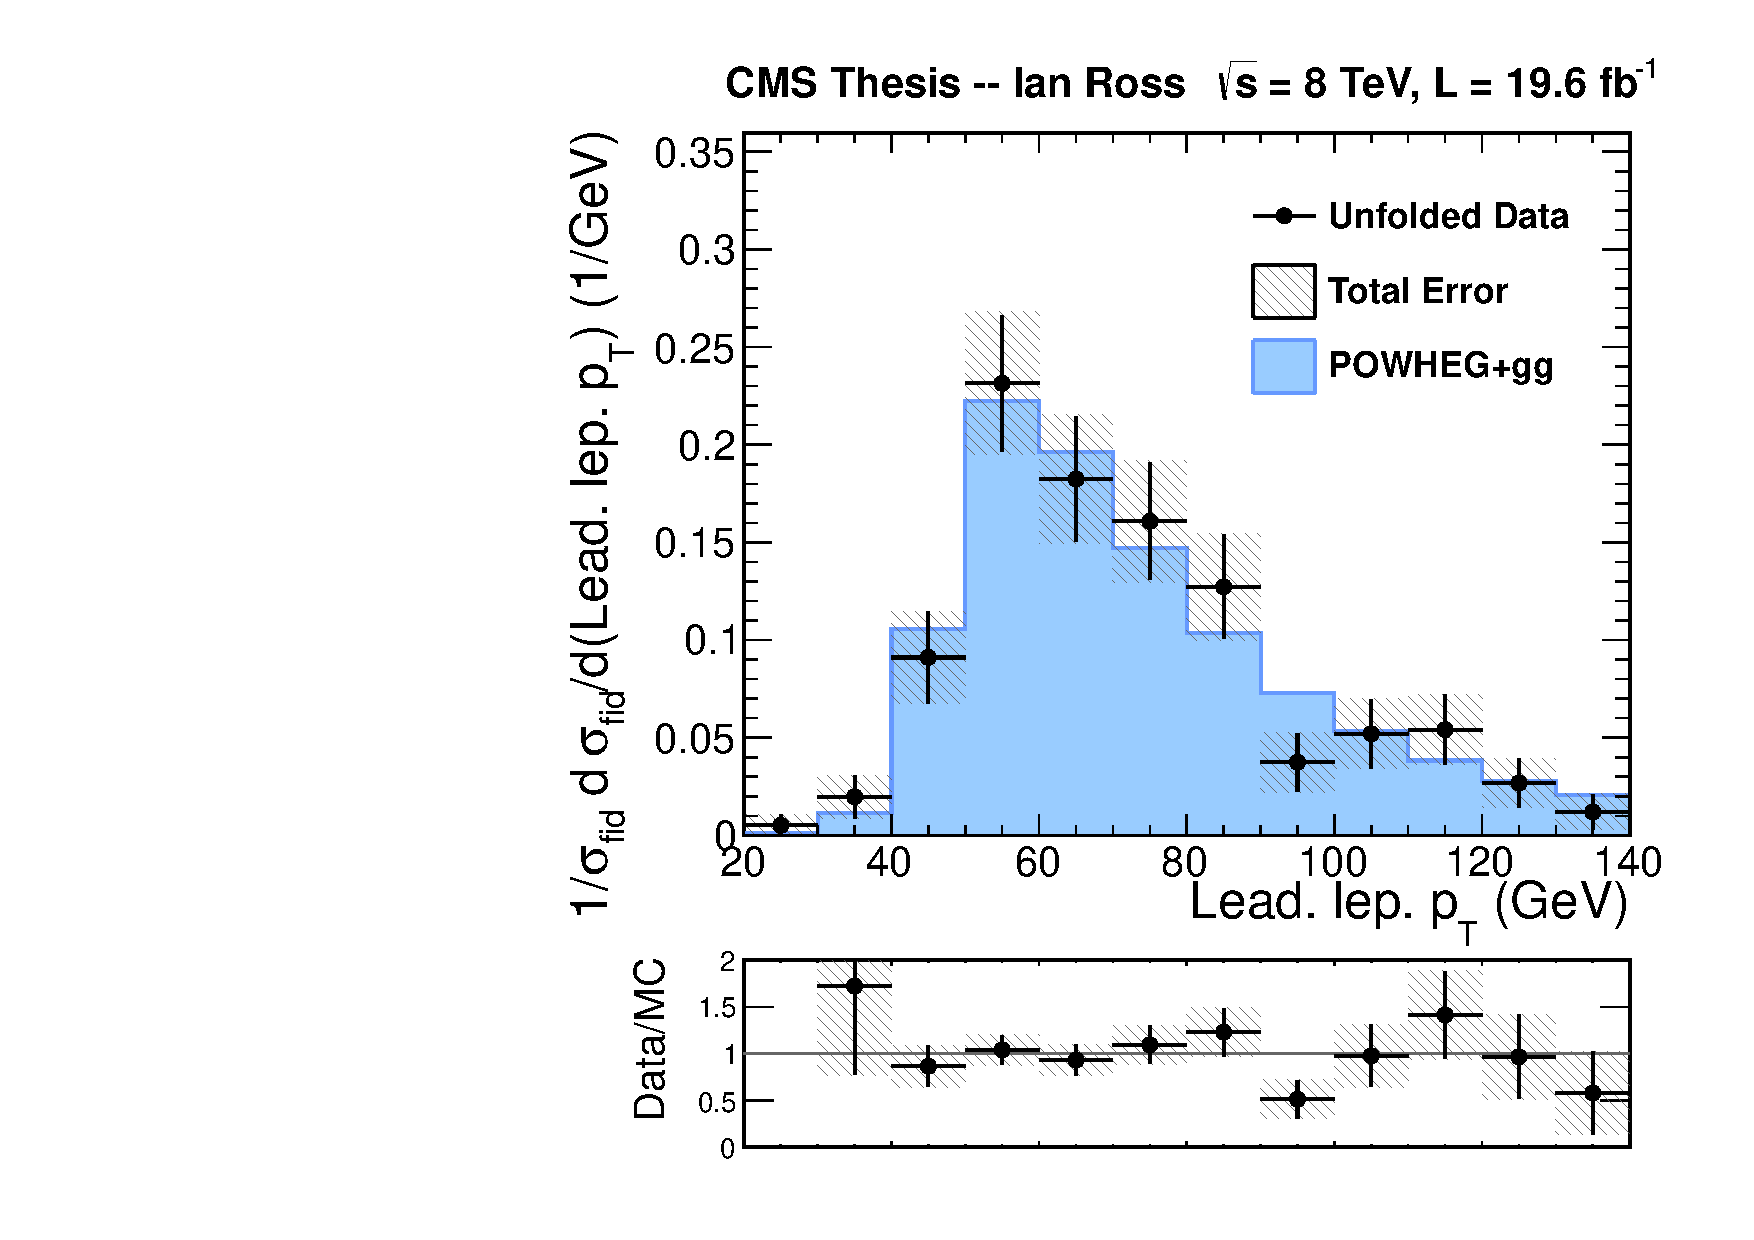
\includegraphics[width=0.75\textwidth]{leadingLep_pt}
\caption[Unfolded distribution of the highest $p_T$ lepton.]{Unfolded
distribution of the highest lepton $p_T$.}
\label{fig:unfolding_leadingLepPt}
\end{figure}

\begin{figure}[h]
\centering
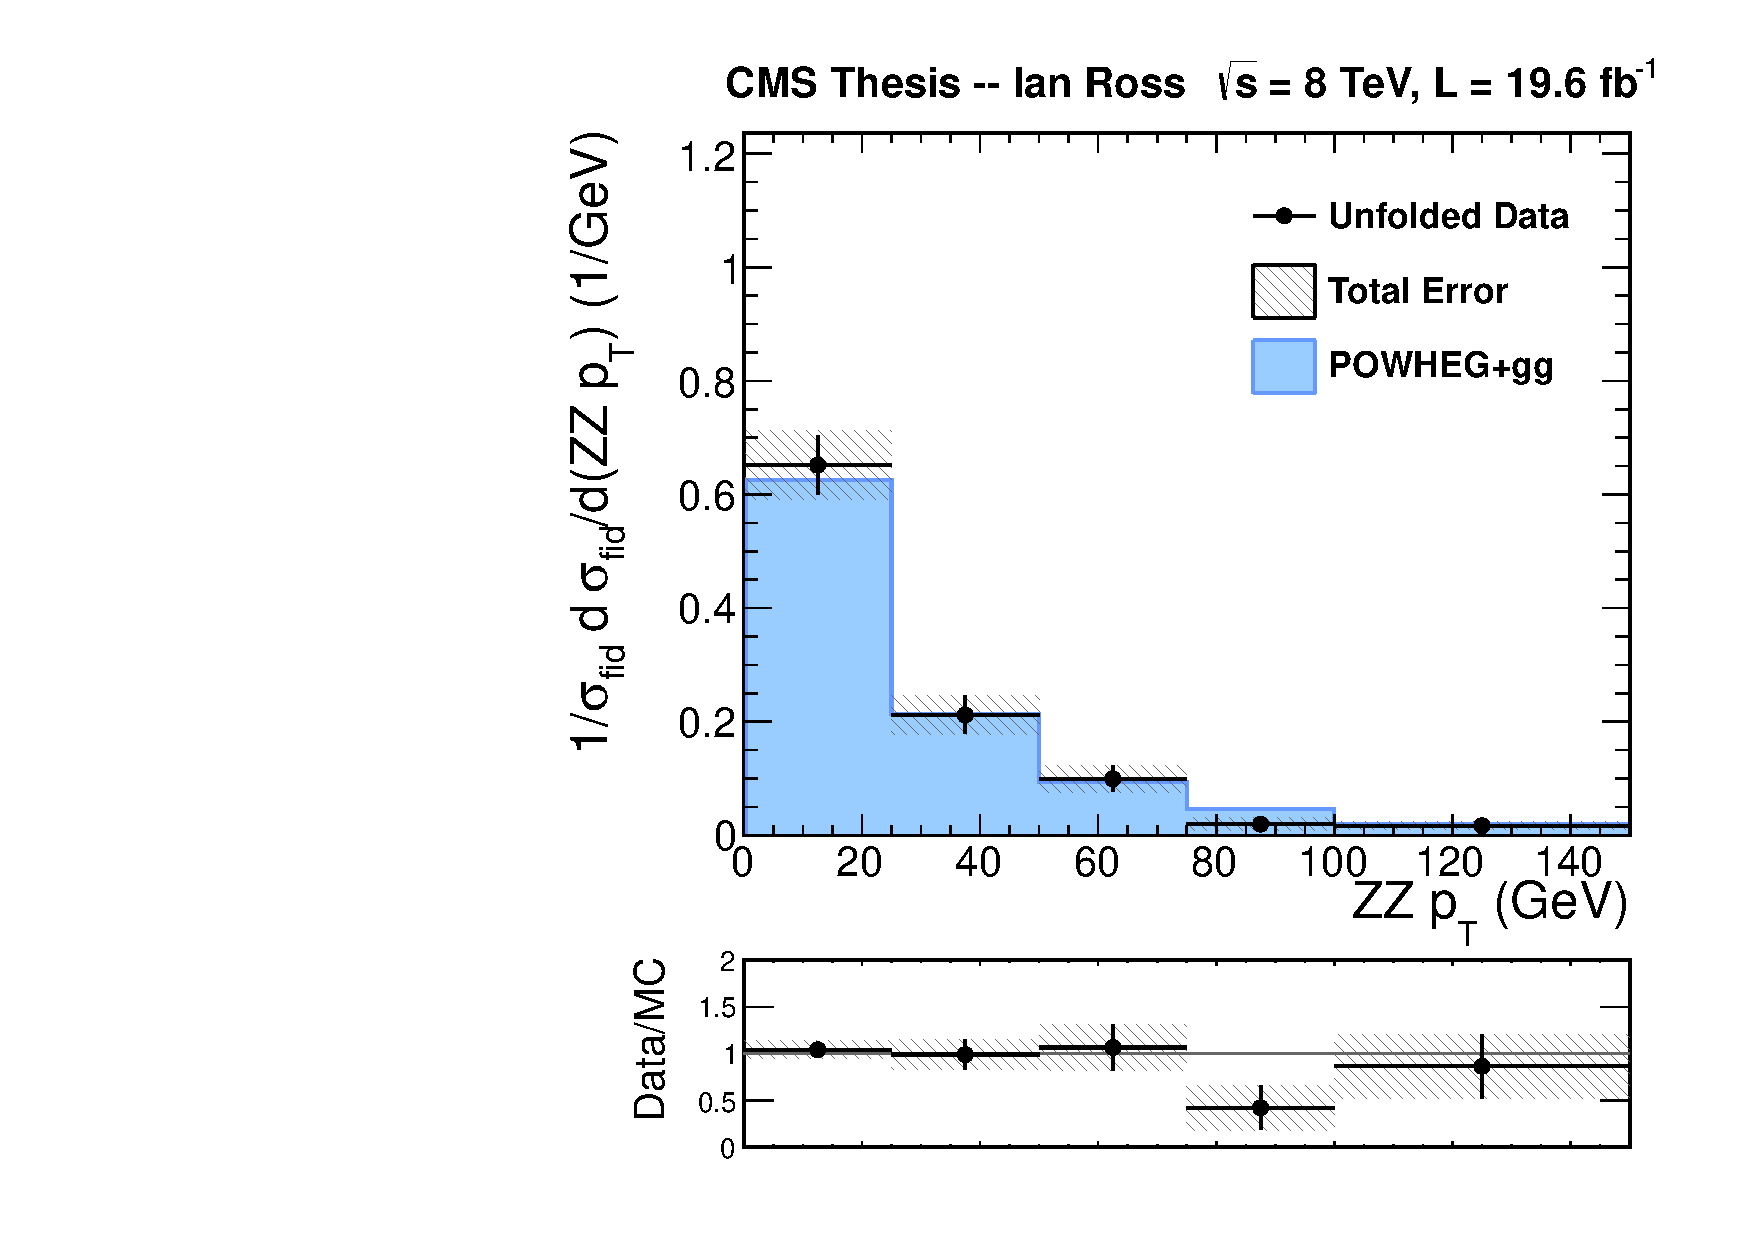
\includegraphics[width=0.75\textwidth]{llll_pt} \\
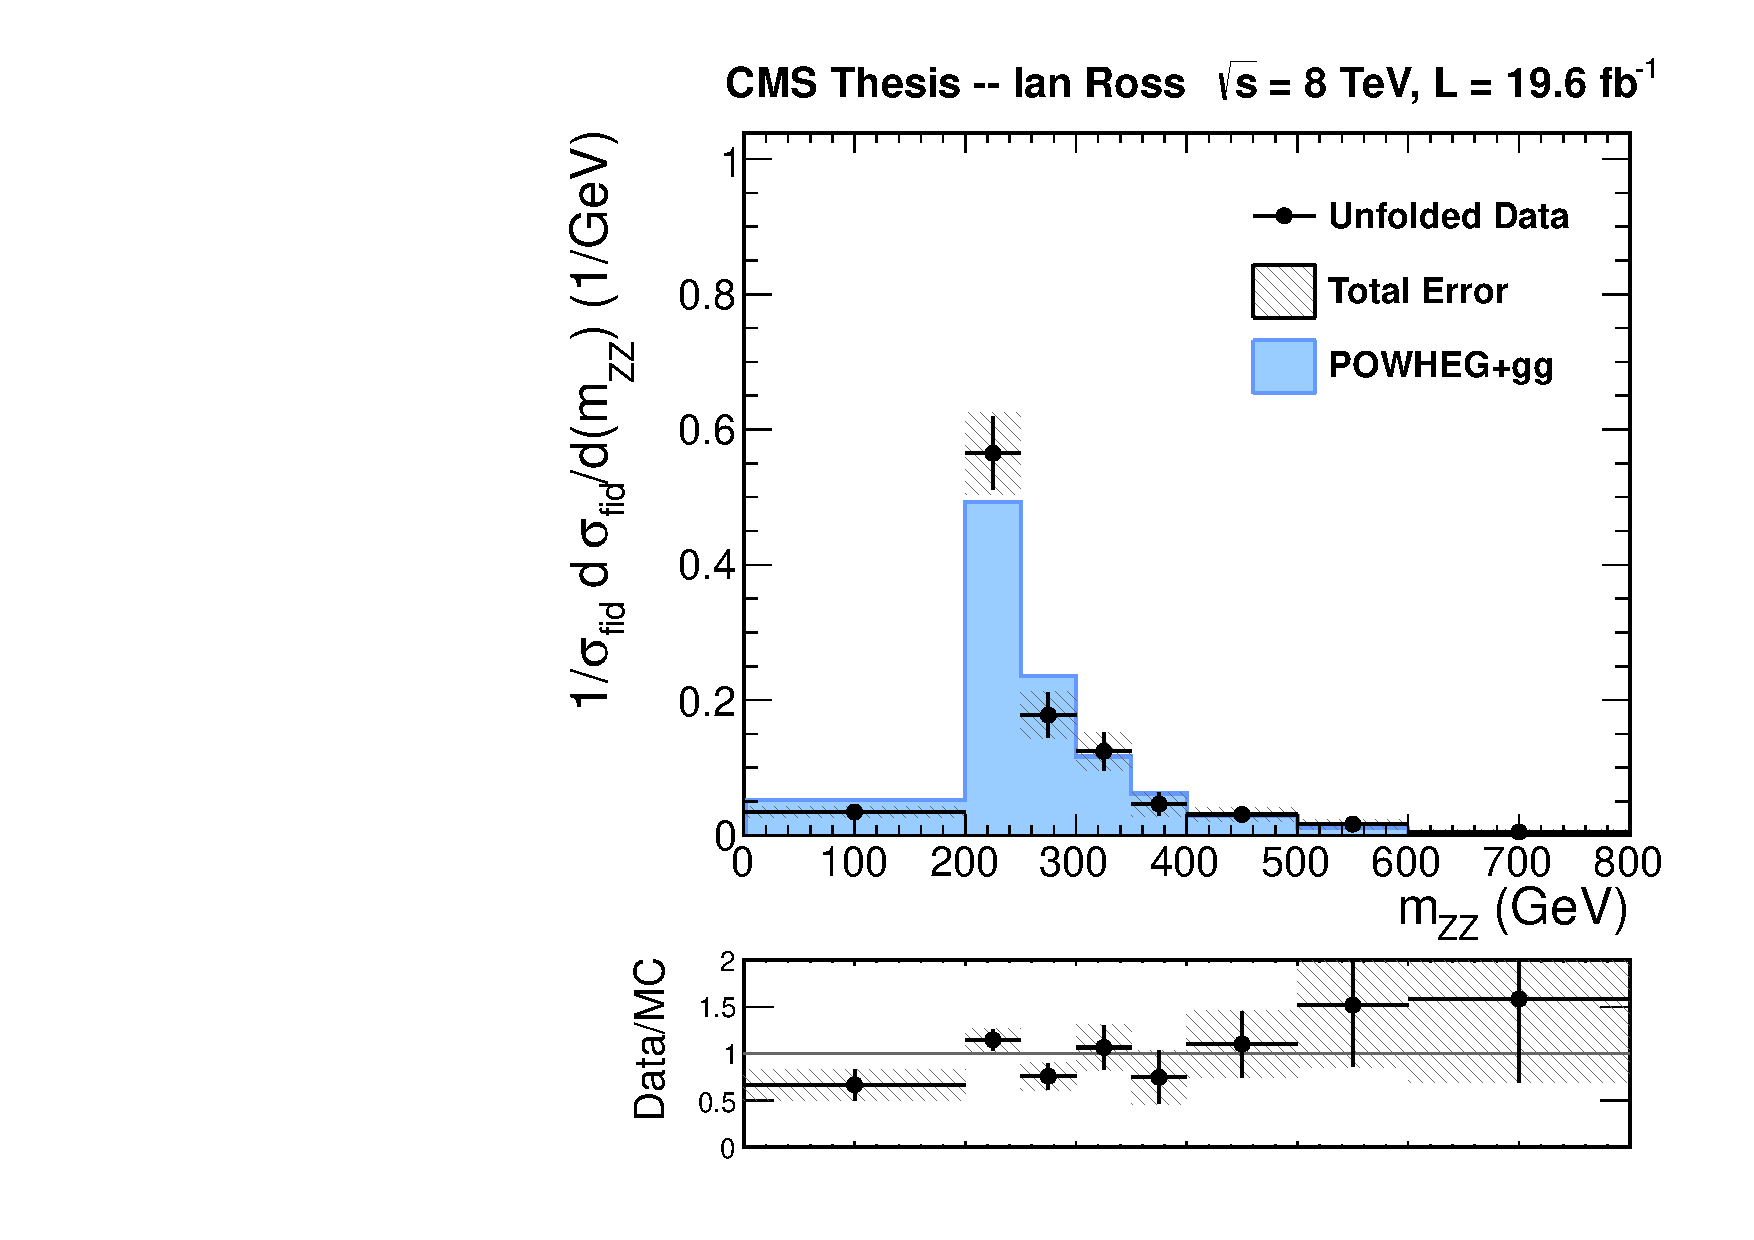
\includegraphics[width=0.75\textwidth]{llll_mass}
\caption[Unfolded ZZ kinematic variables.]{Unfolded ZZ kinematic variables. The
ZZ system $p_{T}$ (top) and $M_{\ell\ell\ell\ell}$ (bottom).}
\label{fig:unfolding_ZZ}
\end{figure}

\begin{figure}[h]
\centering
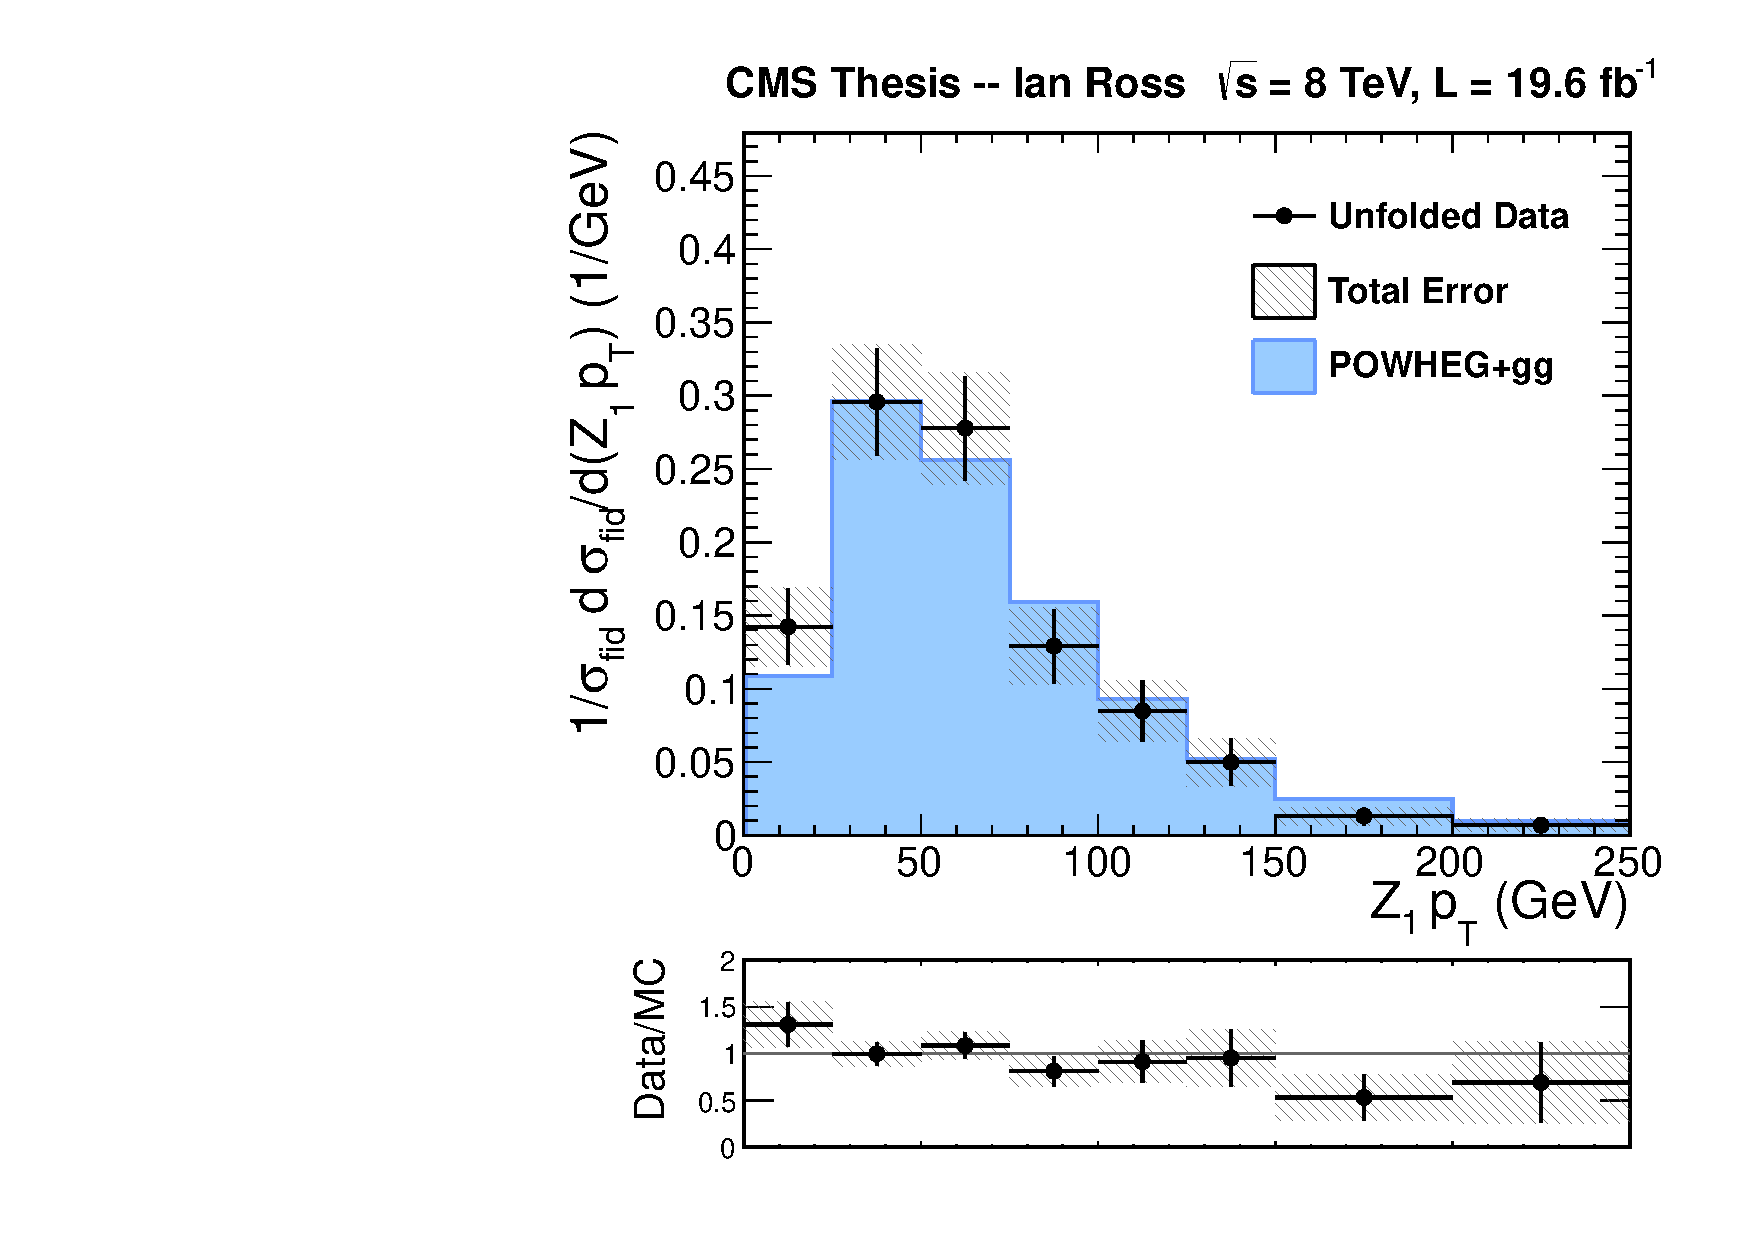
\includegraphics[width=0.75\textwidth]{llll_leadingZpt} \\ 
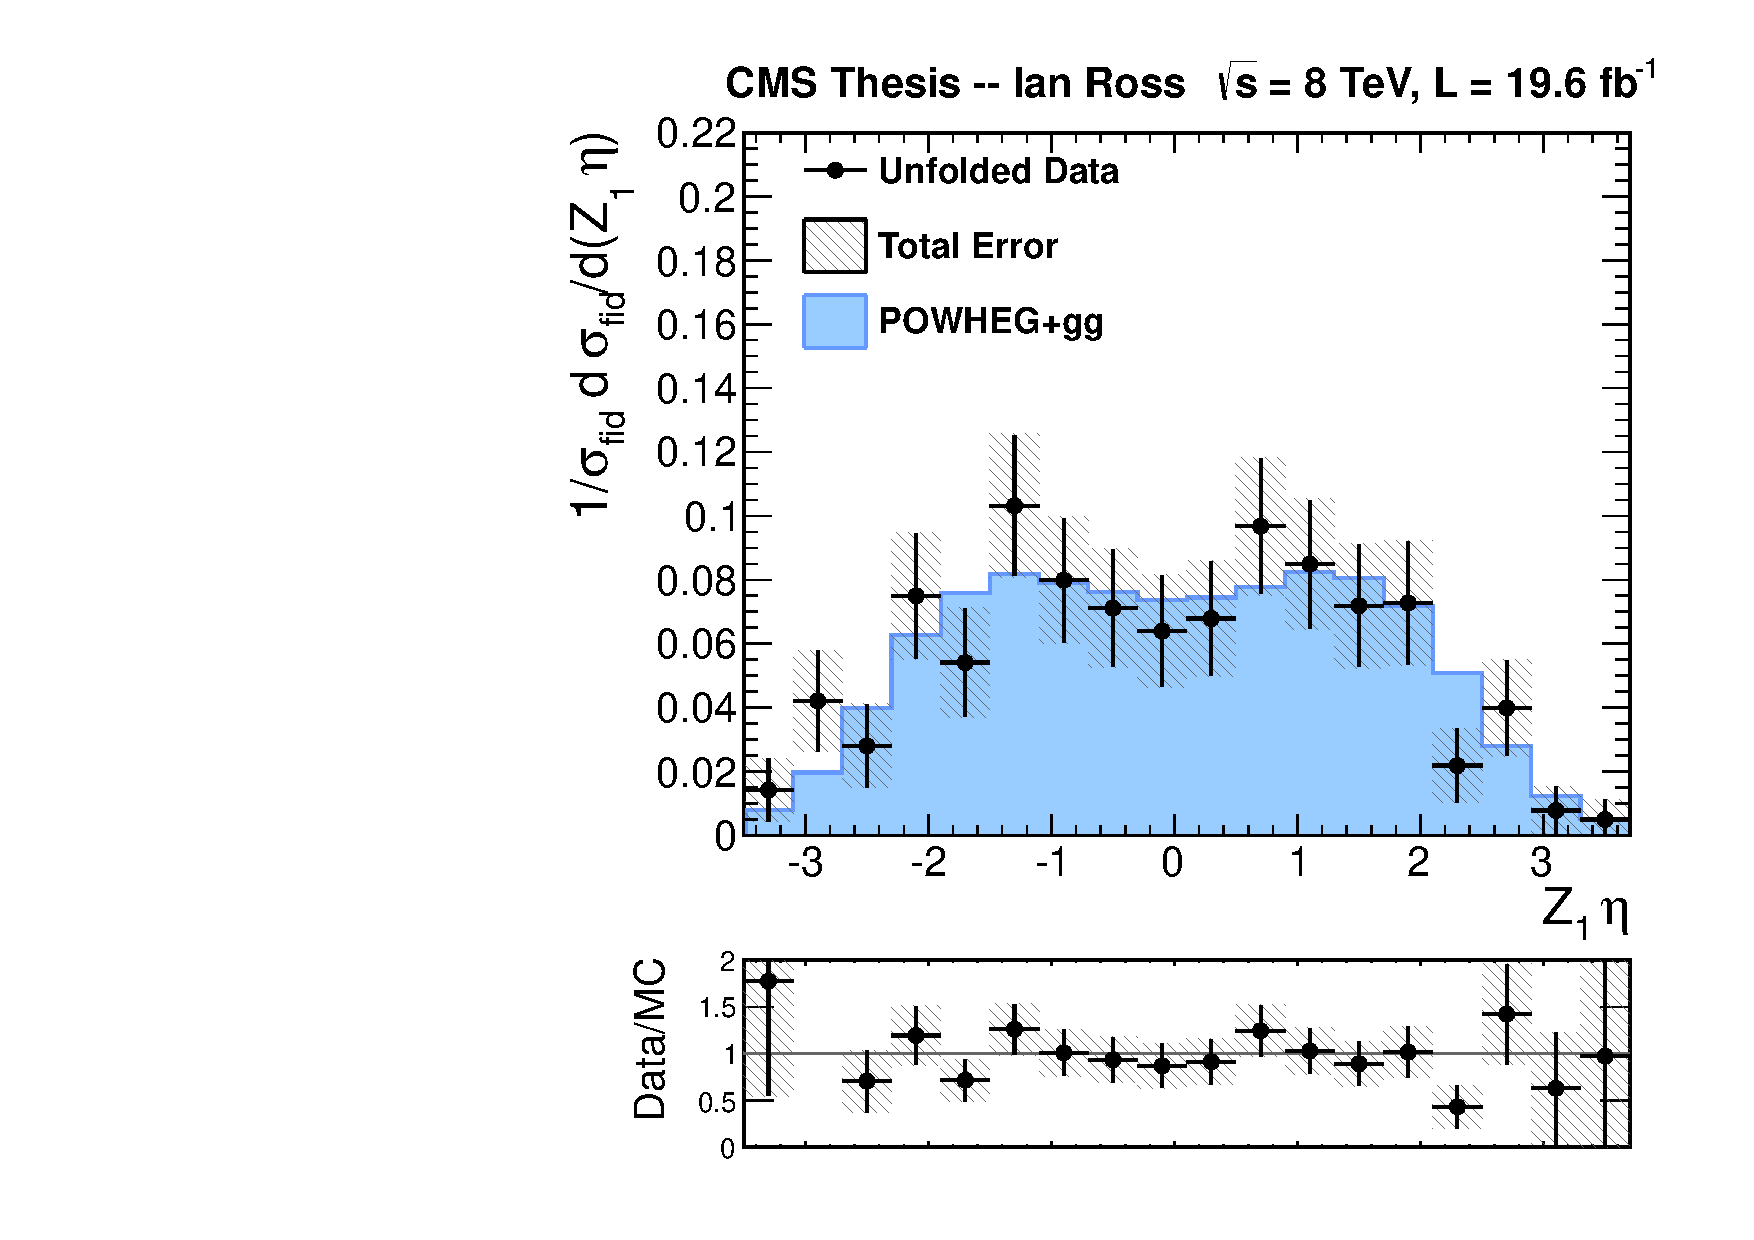
\includegraphics[width=0.75\textwidth]{llll_leadingZeta}
\caption[Unfolded leading (in $p_T$) Z kinematic variables.]{Unfolded leading (in
$p_T$) kinematic variables. The unfolded
Z system $p_{T}$ (top) and $\eta$ (bottom) distributions.}
\label{fig:unfolding_Z1}
\end{figure}

\begin{figure}[h]
\centering
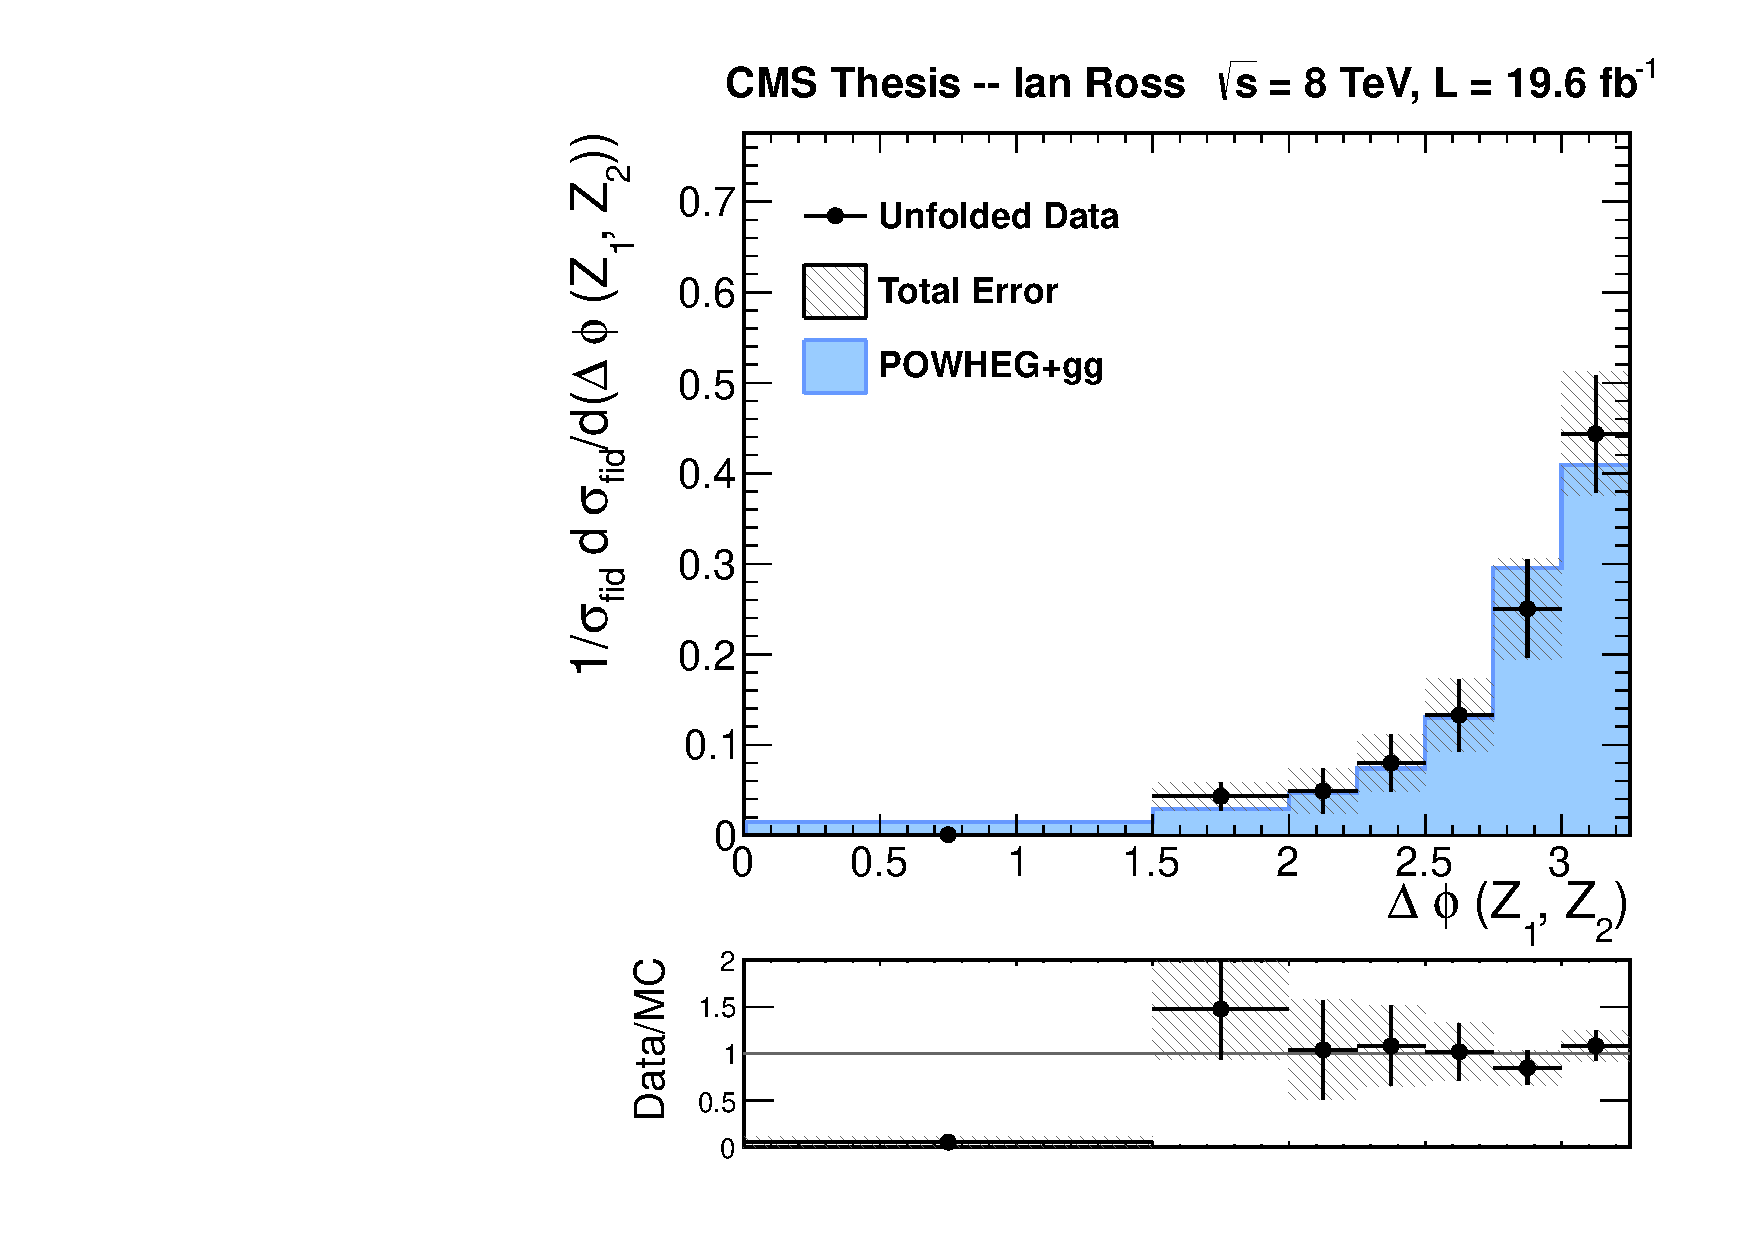
\includegraphics[width=0.75\textwidth]{dPhi_Zs} \\ 
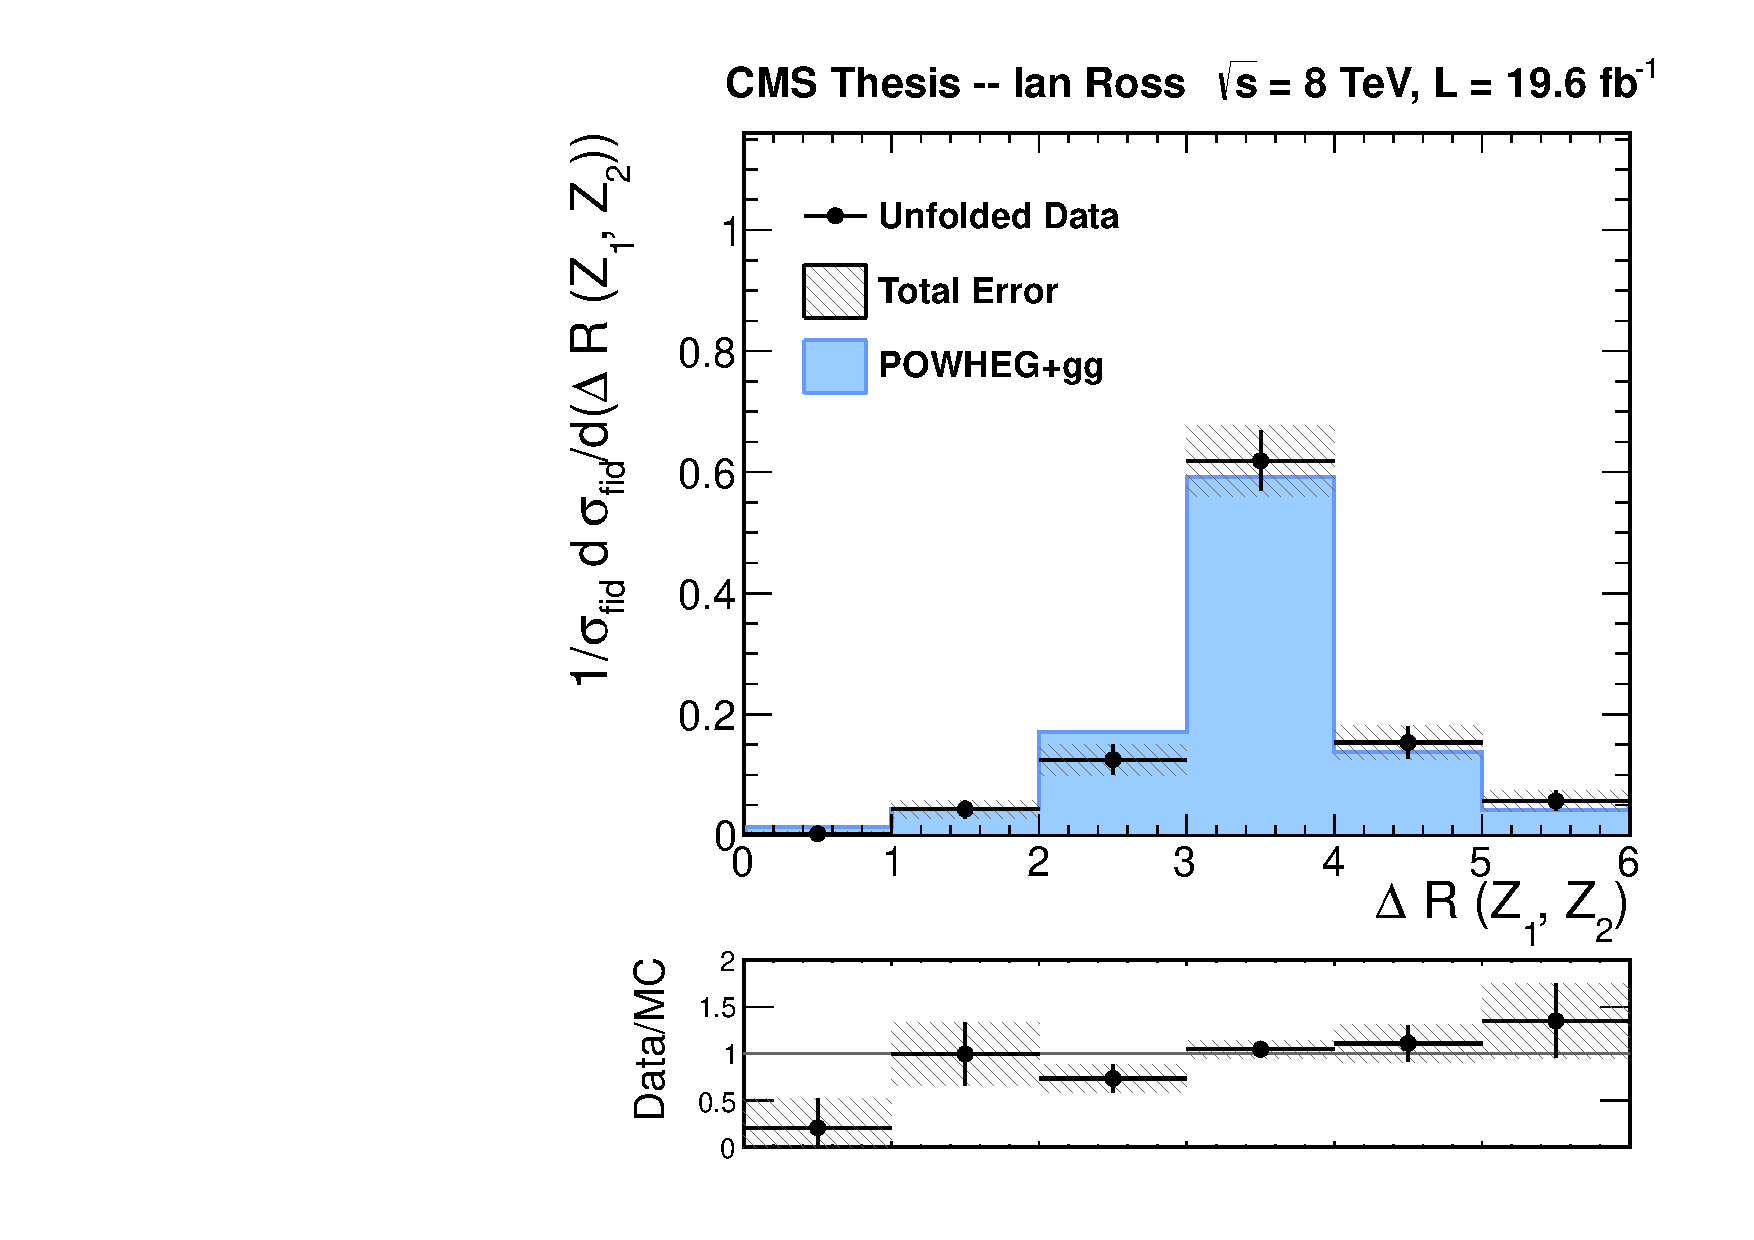
\includegraphics[width=0.75\textwidth]{llll_dR_Z}
\caption[Unfolded distribution of the Z candidate separation.]{Unfolded
distribution of the Z candidate separations, $\Delta \phi$ top and $\Delta R$
bottom.}
\label{fig:unfolding_Z_separation}
\end{figure}


\clearpage

\section{Search for a Standard Model Higgs Boson}
Overall yields for the low-mass (Higgs search) analysis are presented in
Table~\ref{tab:higgsYields}. The observed four-lepton invariant mass across the
entire mass range is presented in Figure~\ref{fig:zzMass_higgs_full}. A
significant excess is observed in the vicinity of 126~GeV, and this region is
shown in finer binning in Figure~\ref{fig:zzMass_higgs_low}.

\begin{table}[h]
\centering
\begin{tabular}{|c|c|c|c|}
\hline
& eeee & $\mu\mu\mu\mu$ & $\mu\mu e e$ \\
\hline
H(126) & $2.86\pm0.03$ & $5.49 \pm 0.05$ & $7.92 \pm 0.06$ \\
H(350) & $11.65 \pm 0.09 $ & $15.80\pm 0.11$ & $27.89 \pm 0.15$ \\
ZZ & $ 68.21 \pm 0.29 $ & $ 101.58 \pm 0.39 $ & $ 167.32 \pm 0.66 $ \\
Z+Jets & $6.70 \pm 0.49$ & $3.46 \pm 0.78$ & $7.82 \pm 0.80$ \\
\hline
BG Expected & 74.91 & 105.04 & 175.14 \\
\hline
Observed & 73 & 109 & 194 \\
\hline
\end{tabular}
\caption[Final yields per event channel in the low-mass analysis (search for the
Higgs boson).]{Final yields per event channel in the low-mass analysis (search for the
Higgs boson). Errors are statistical only.} 
\label{tab:higgsYields}
\end{table}

\begin{figure}[h]
\centering
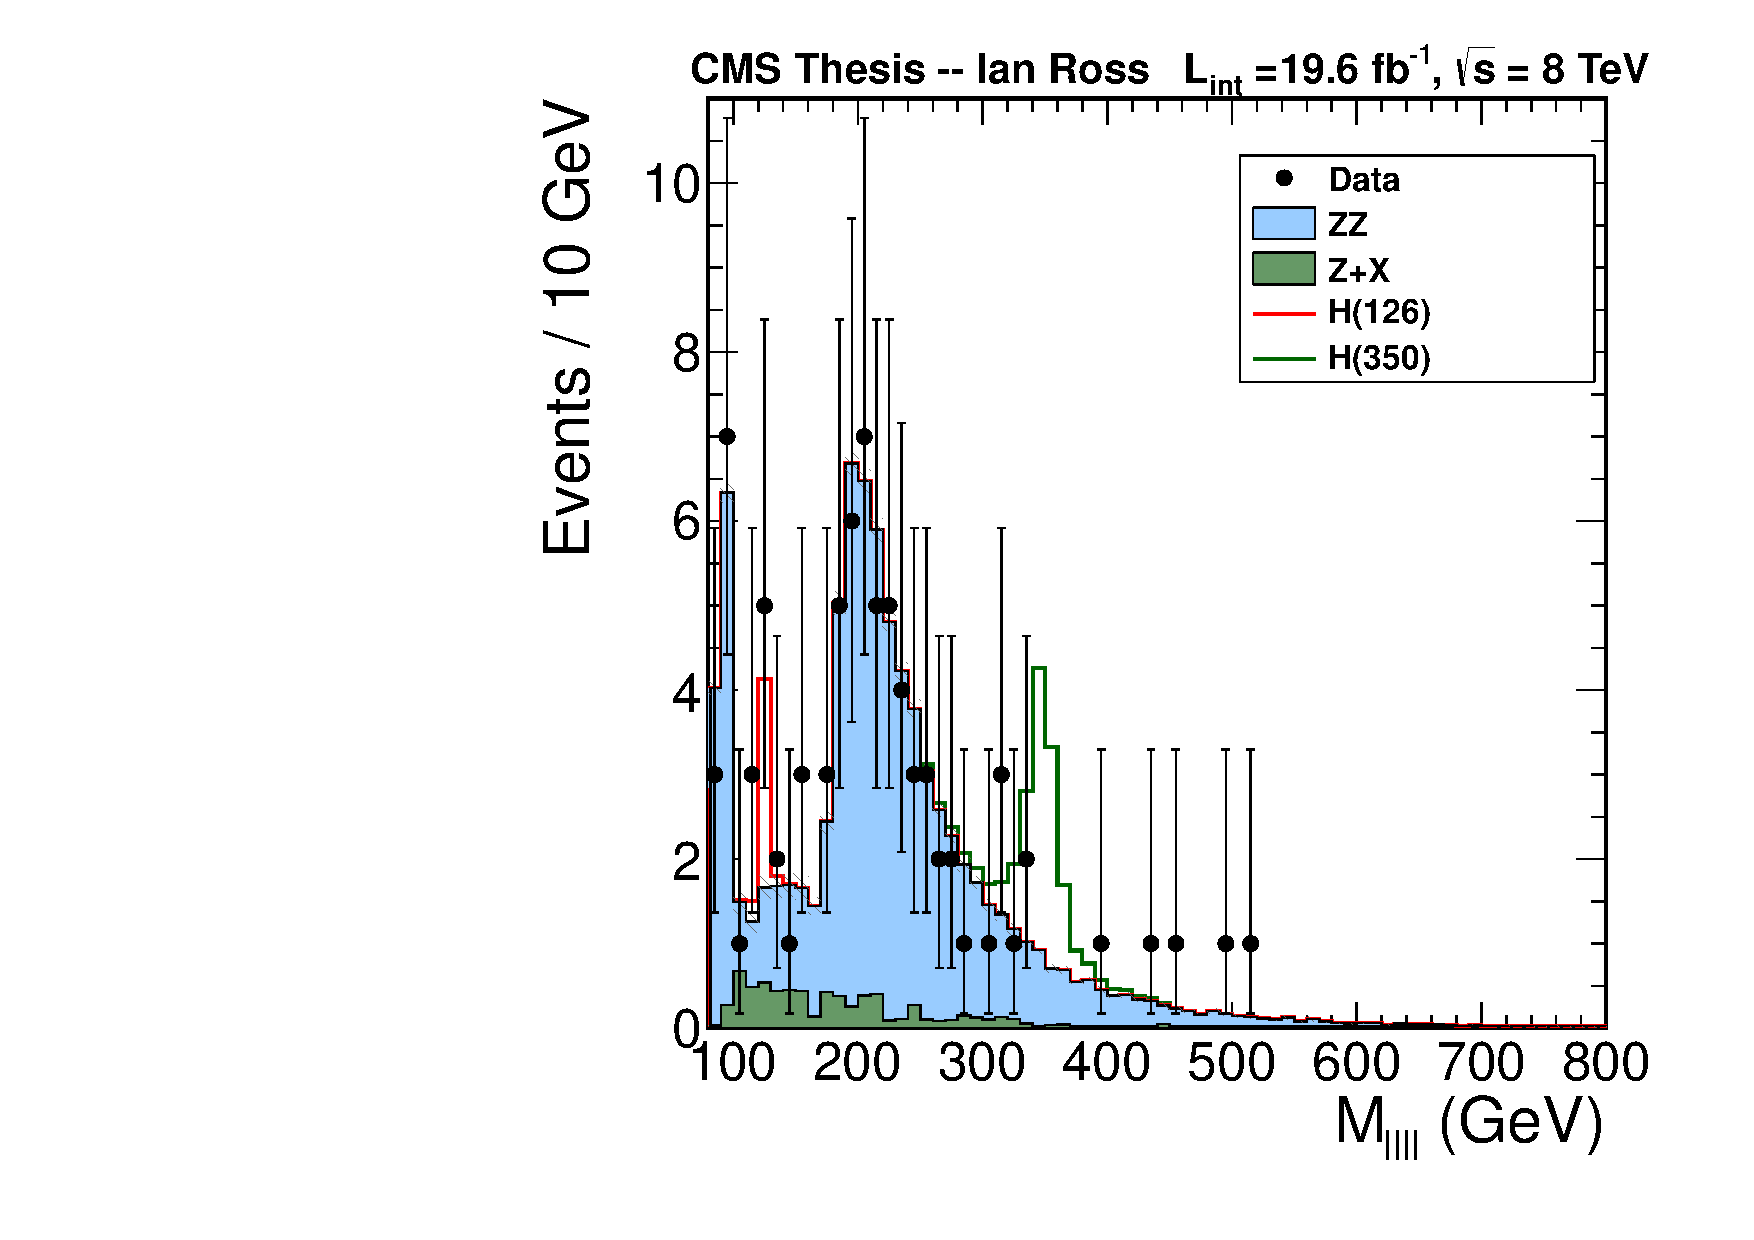
\includegraphics[width=0.40\textwidth]{eeee_mass_full}
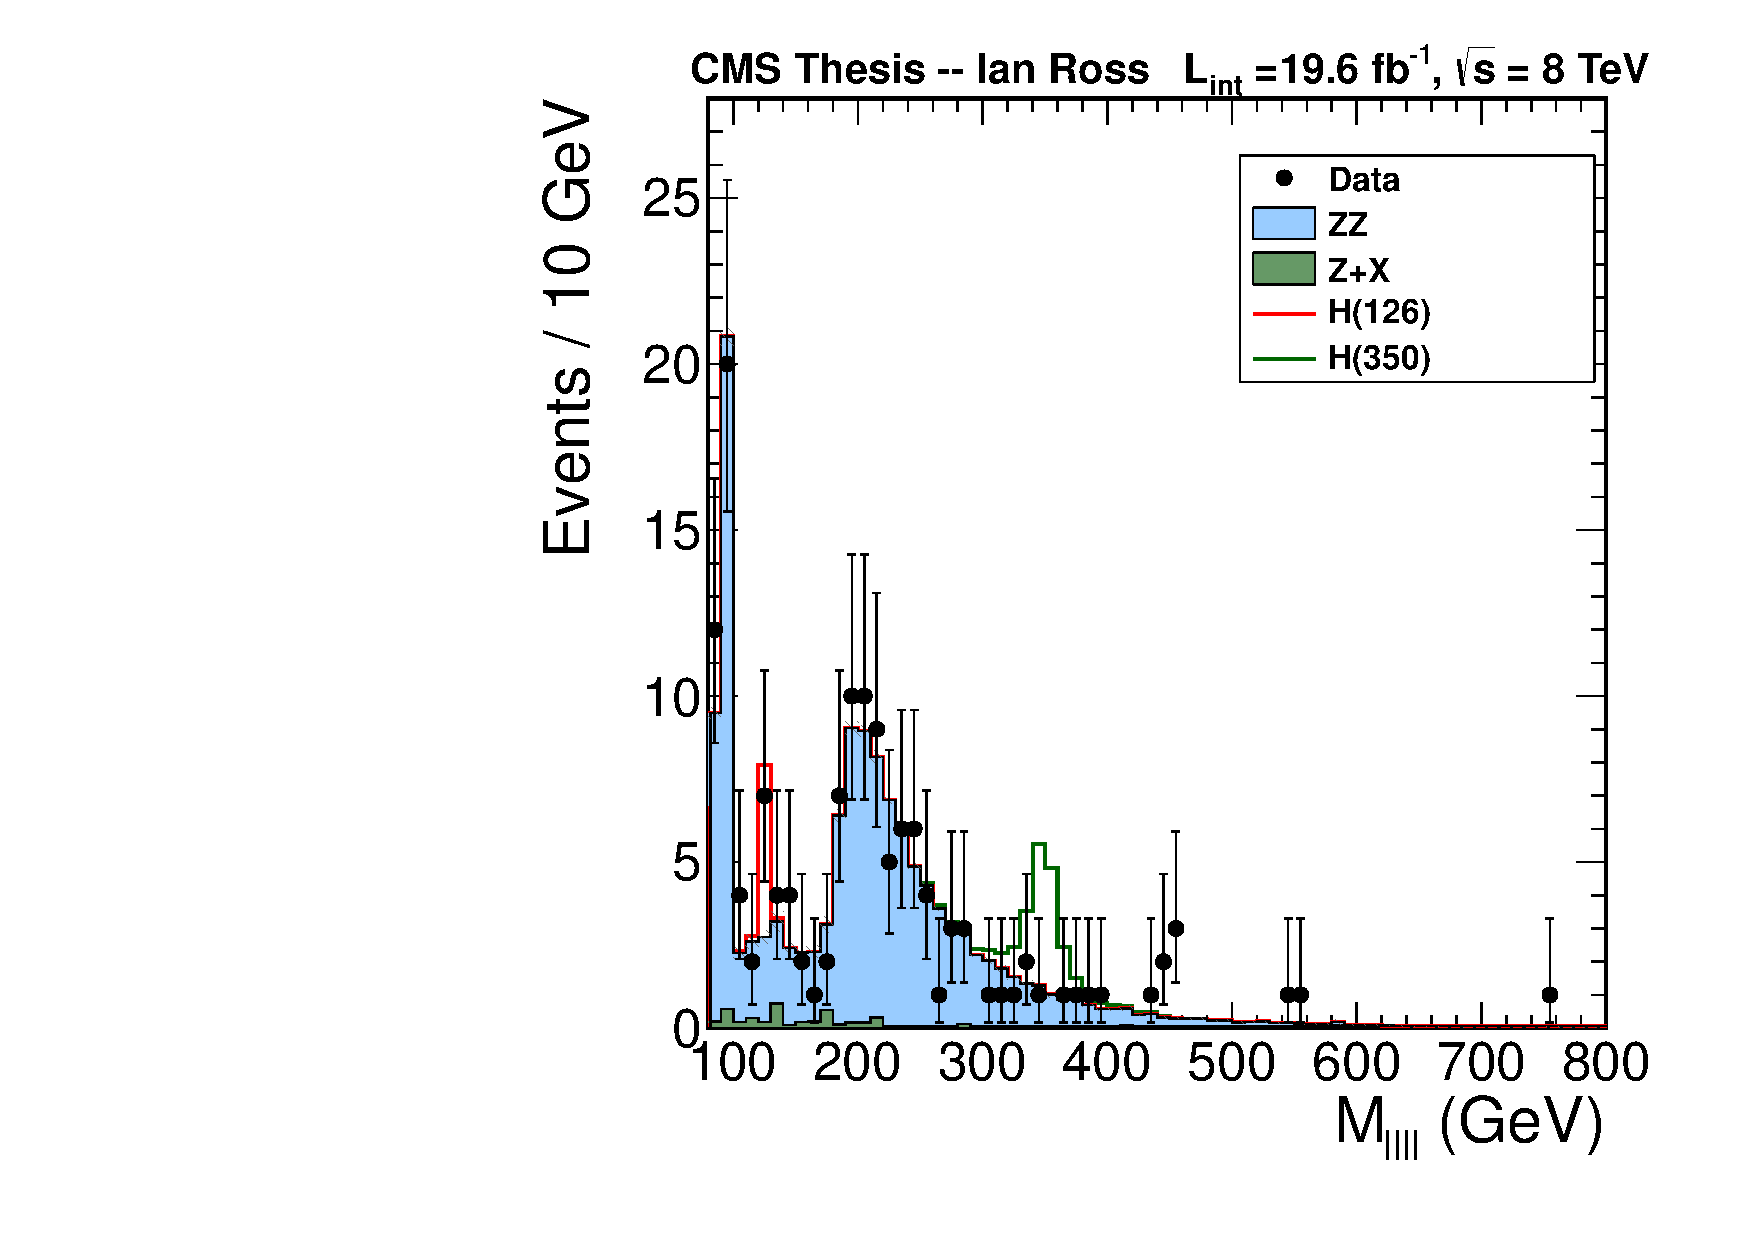
\includegraphics[width=0.40\textwidth]{mmmm_mass_full}\\
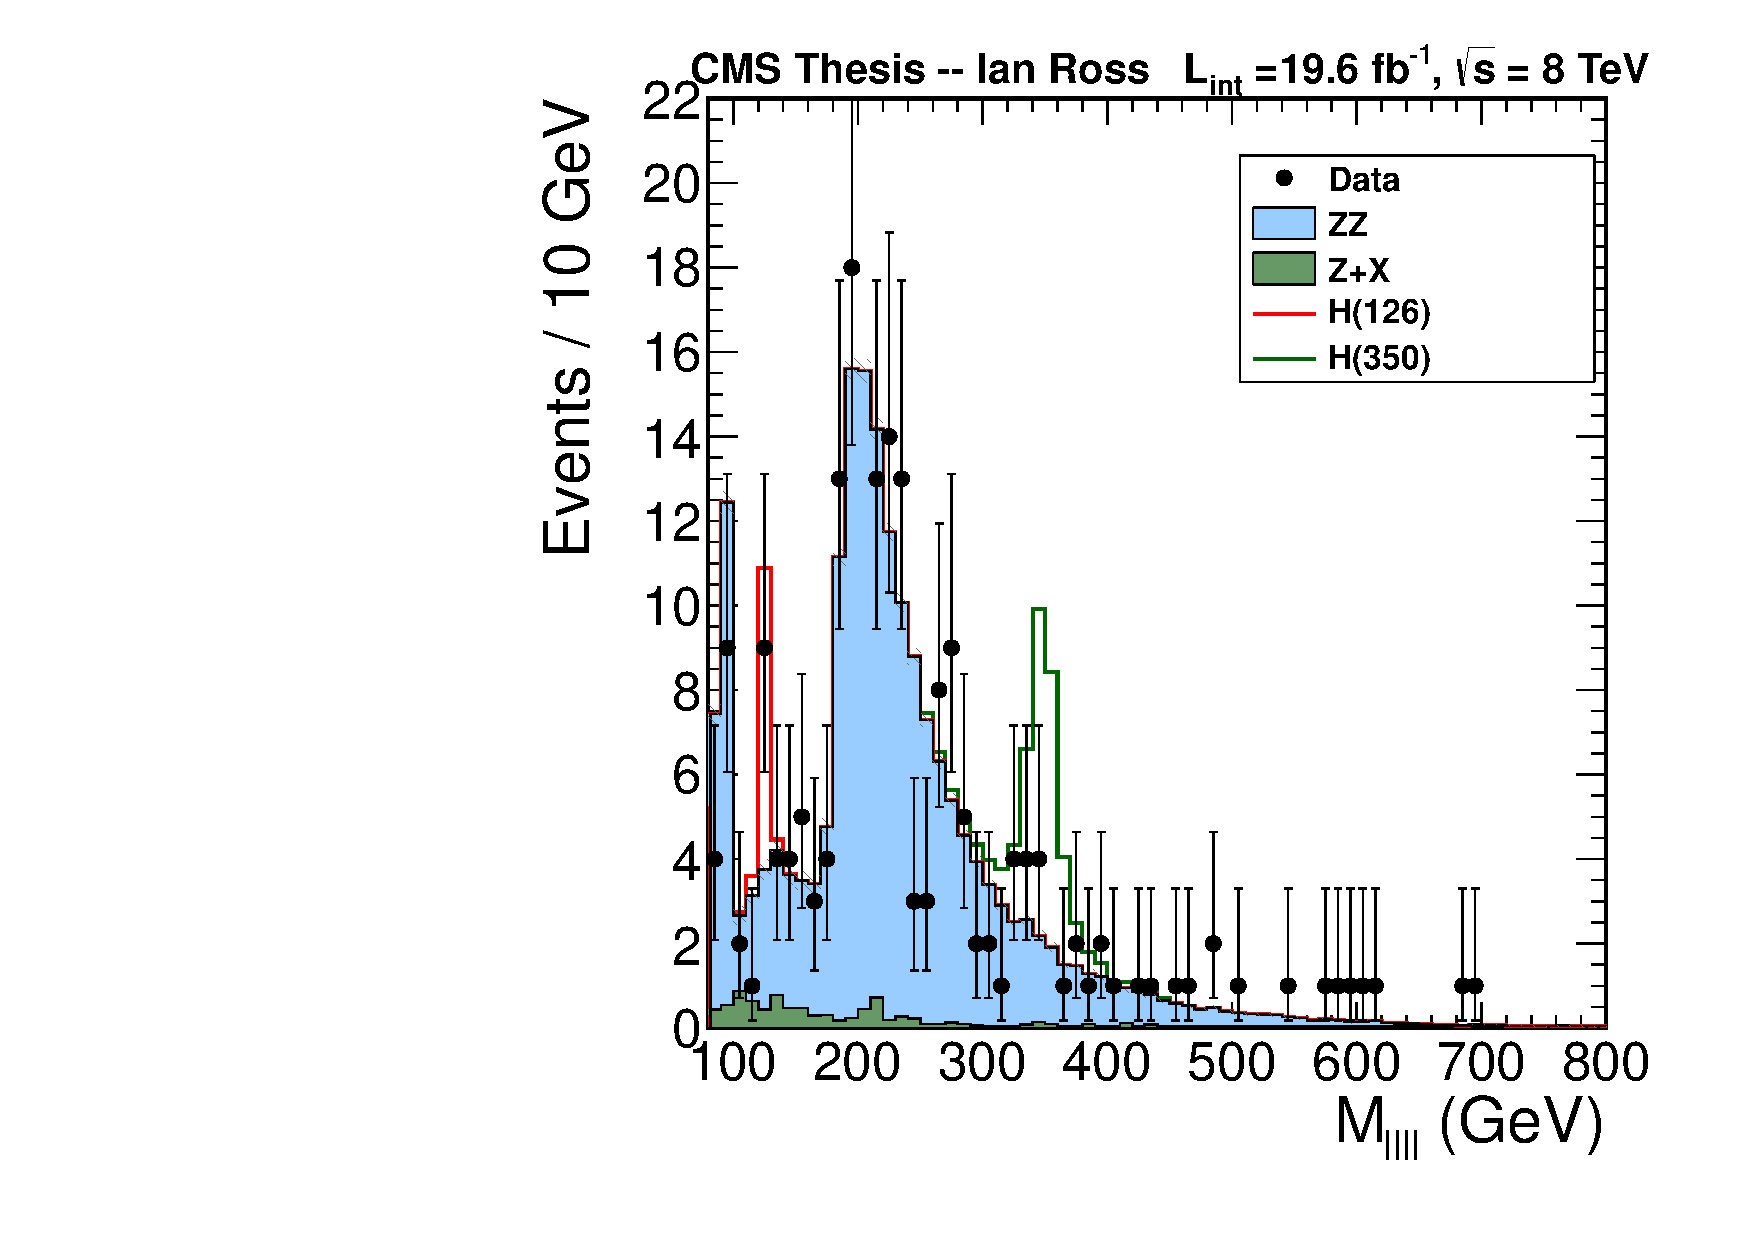
\includegraphics[width=0.40\textwidth]{eemm_mass_full}
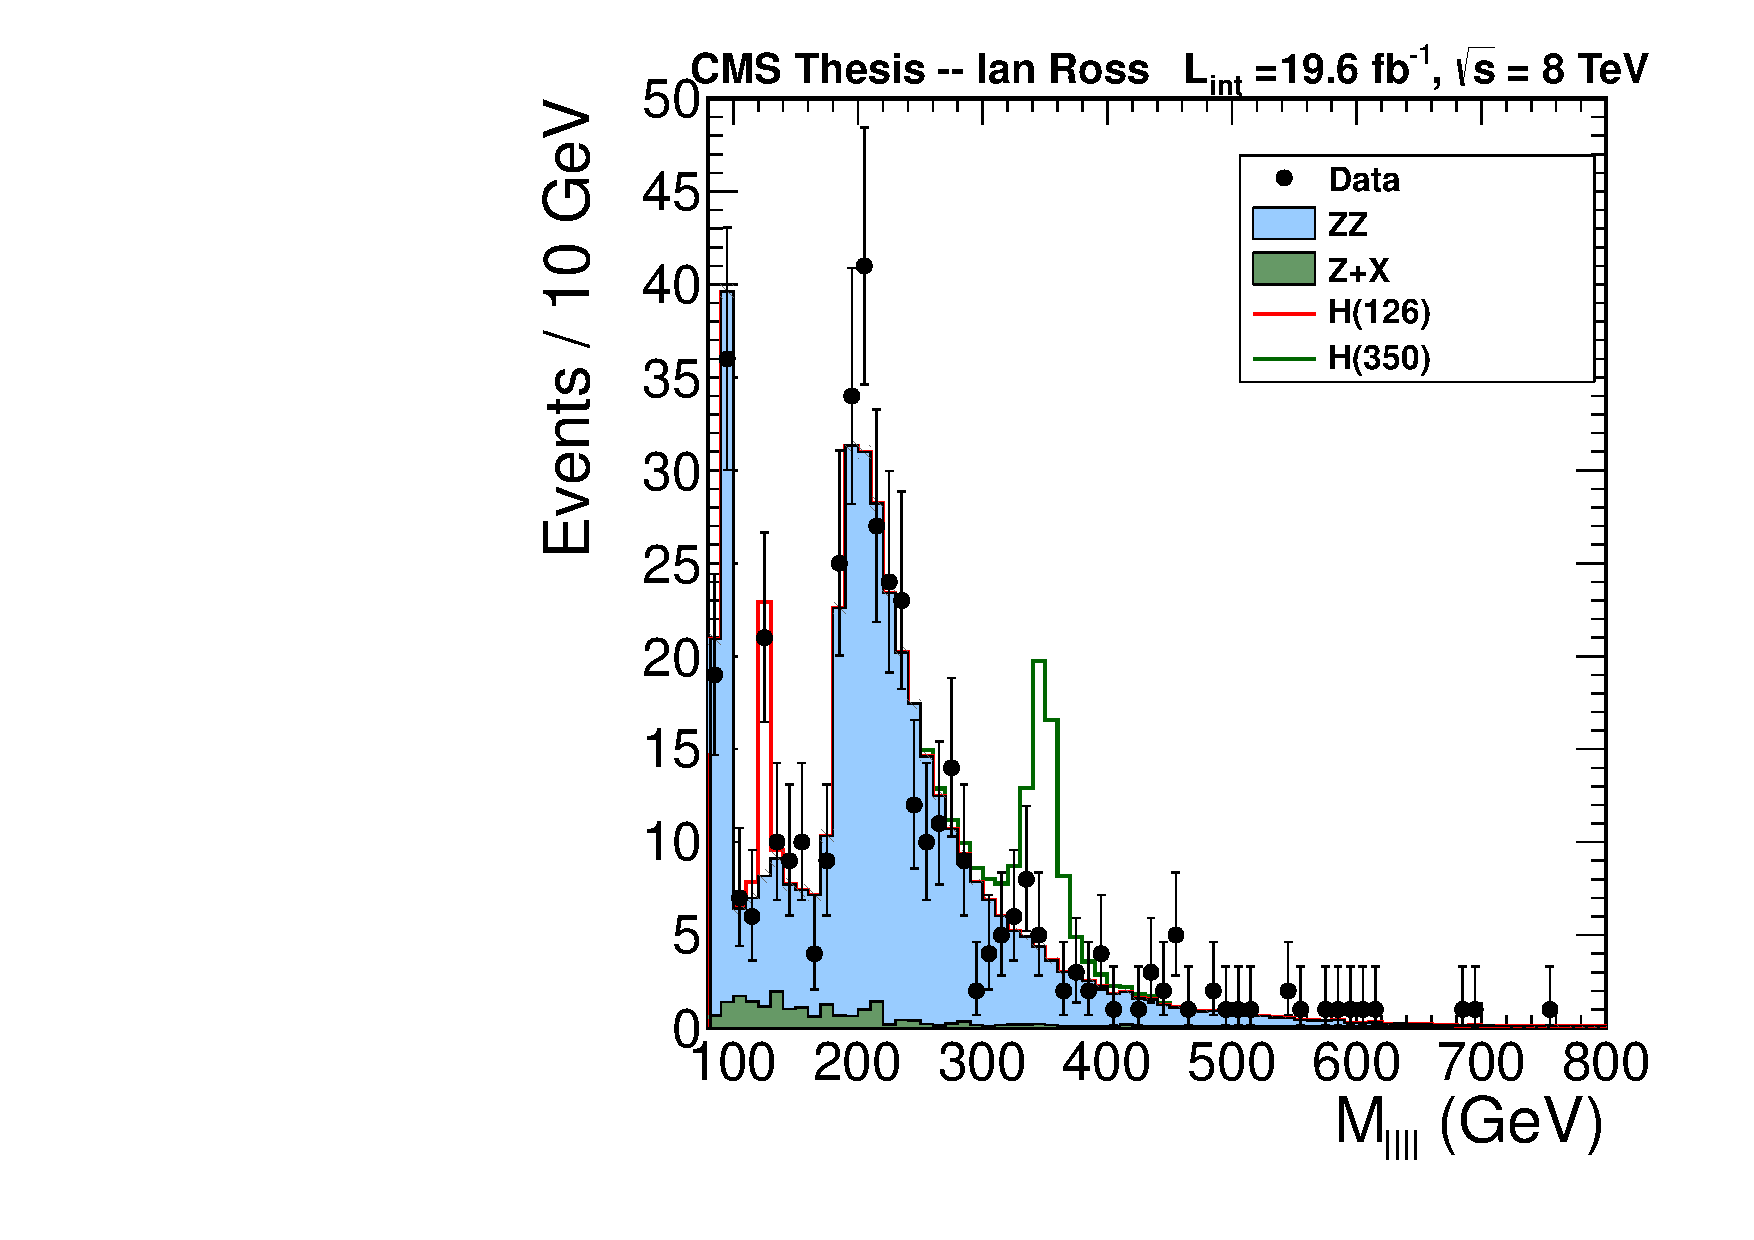
\includegraphics[width=0.40\textwidth]{4l_mass_full}
\caption[ZZ invariant mass for the low-mass analysis, across the full considered
$M_{\ell\ell\ell\ell}$ range.]{ZZ invariant mass for the low-mass analysis, across the full considered
$M_{\ell\ell\ell\ell}$ range. 
Pictured are the eeee, $\mu\mu\mu\mu$, $\mu\mu e
e$, and combined total results (upper left, upper right, lower left, and lower
right respectively).}
\label{fig:zzMass_higgs_full}
\end{figure}

\begin{figure}[h]
\centering
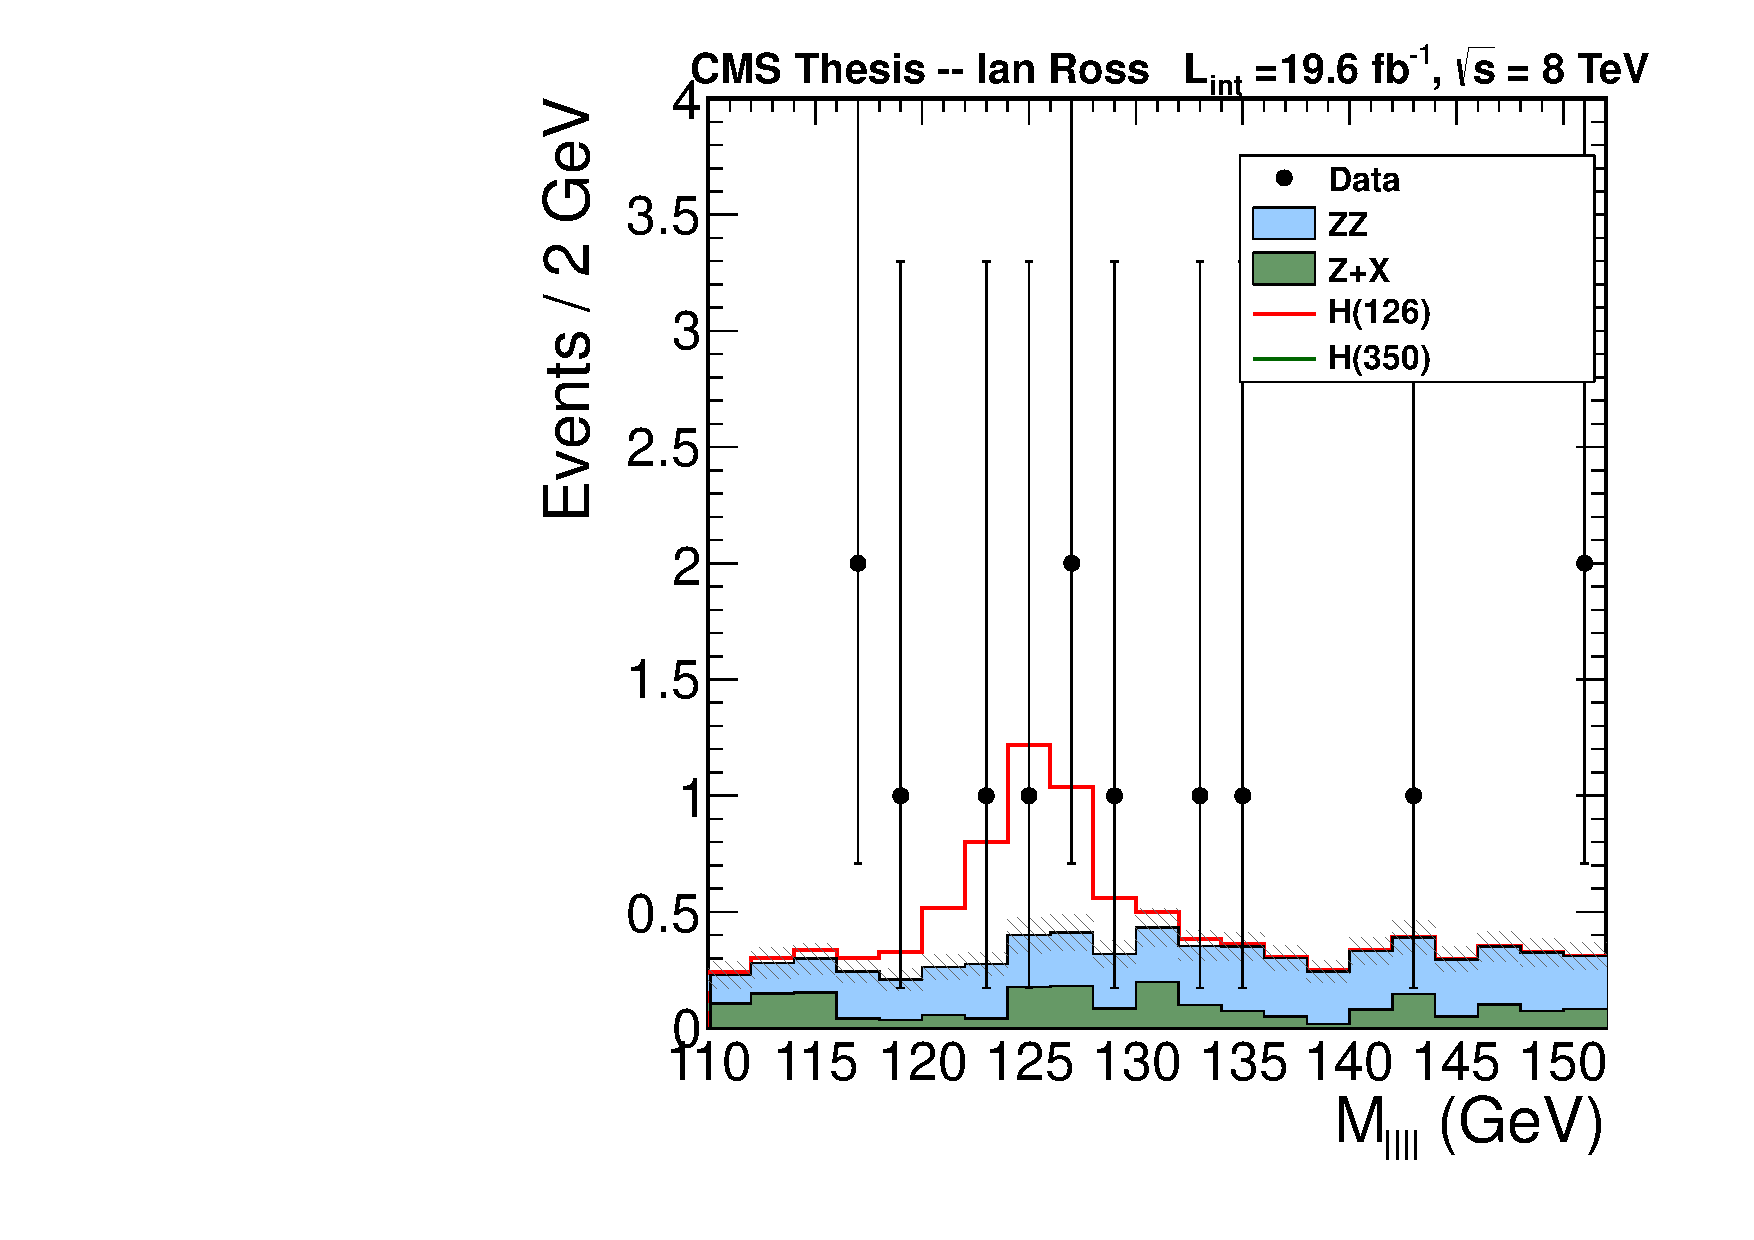
\includegraphics[width=0.40\textwidth]{eeee_mass_low}
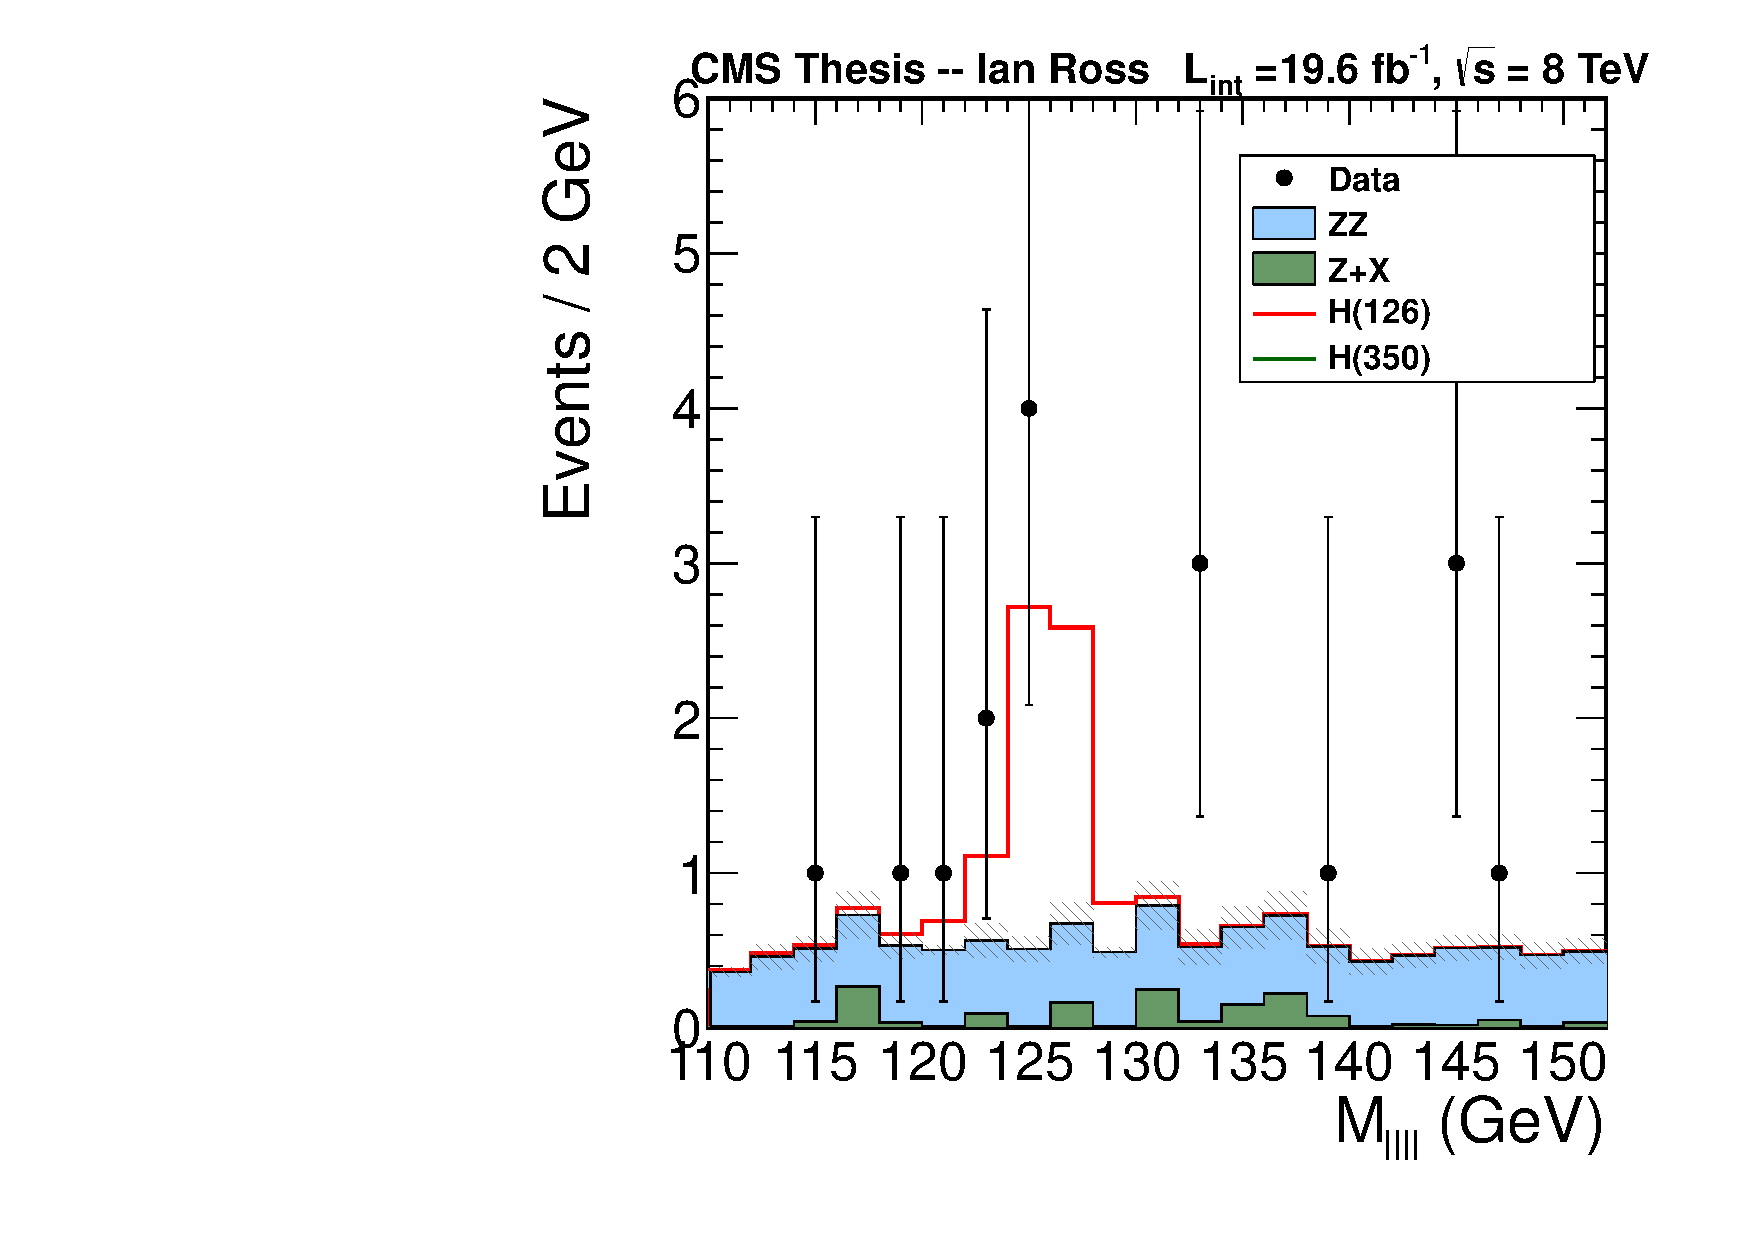
\includegraphics[width=0.40\textwidth]{mmmm_mass_low}\\
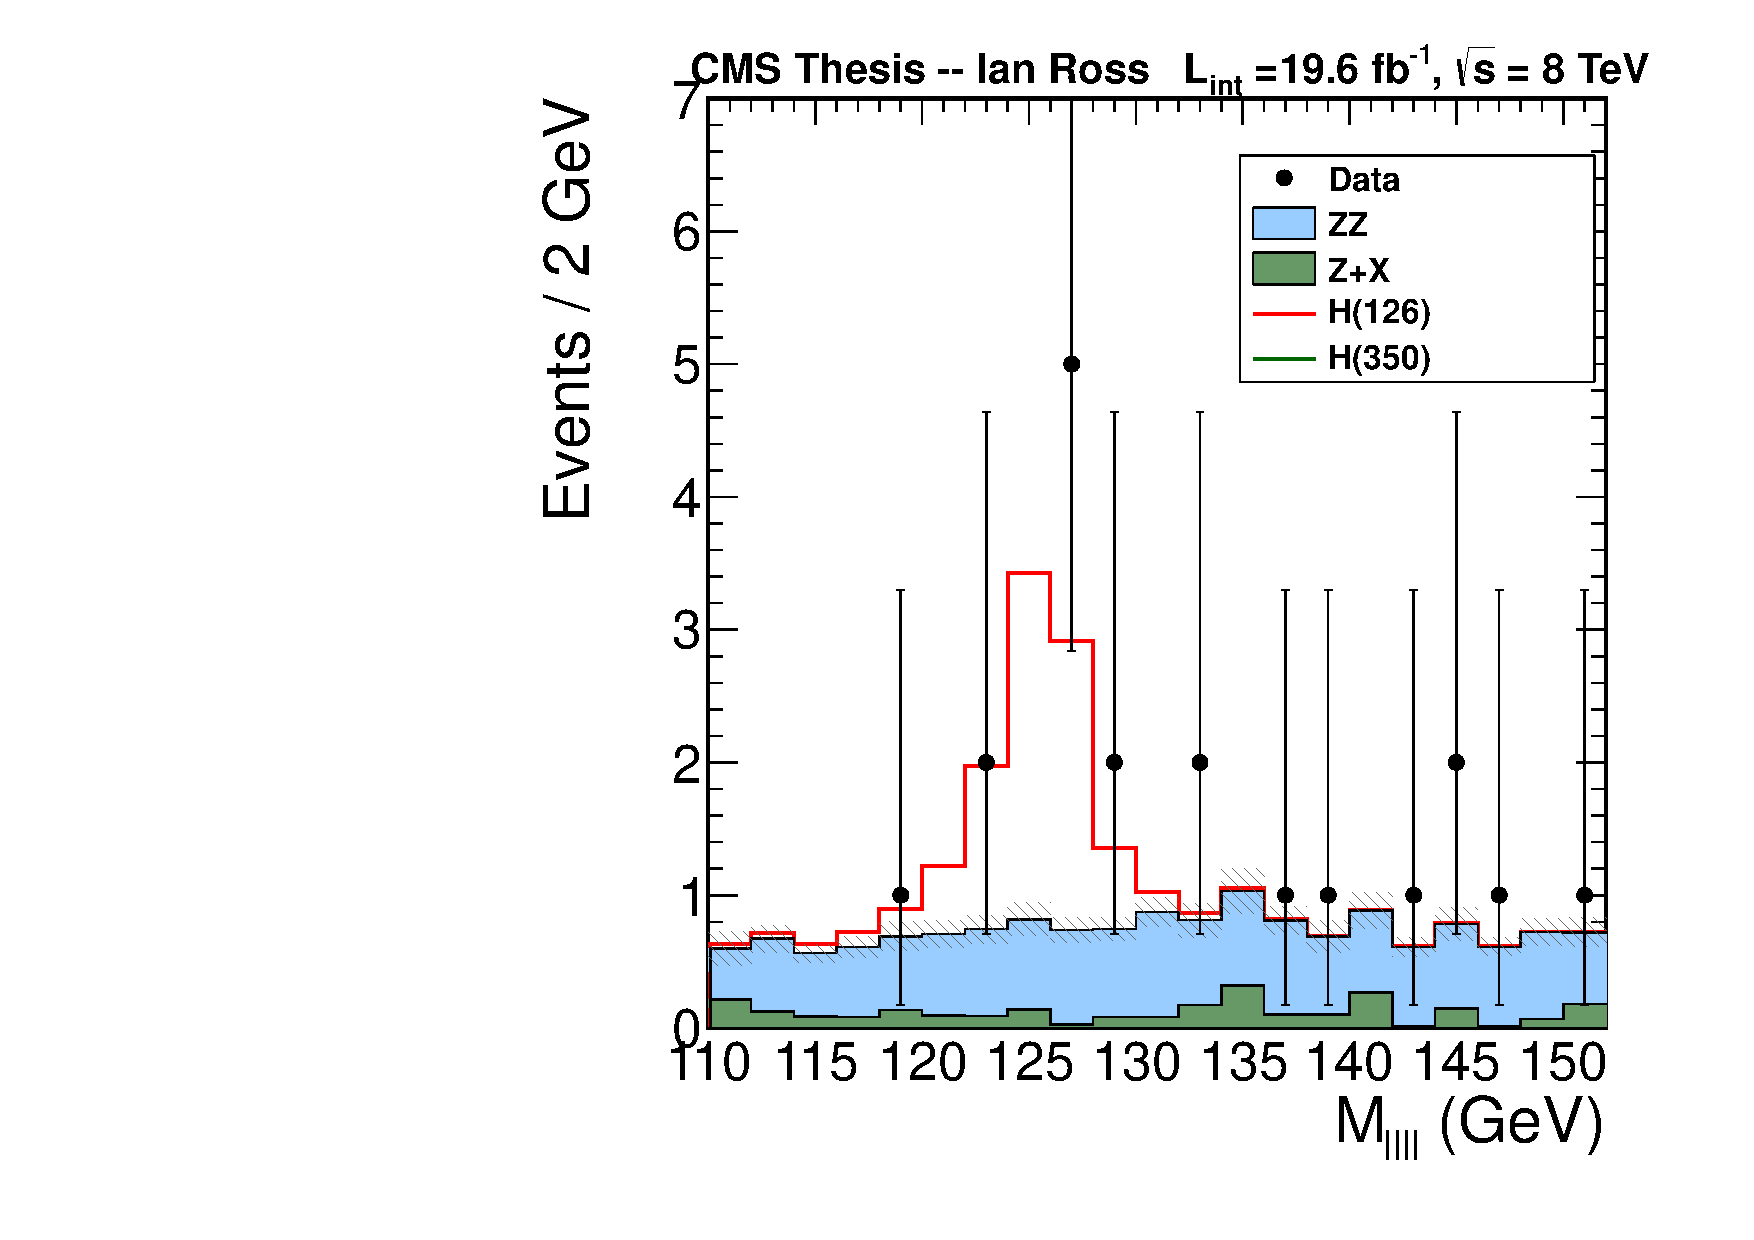
\includegraphics[width=0.40\textwidth]{eemm_mass_low}
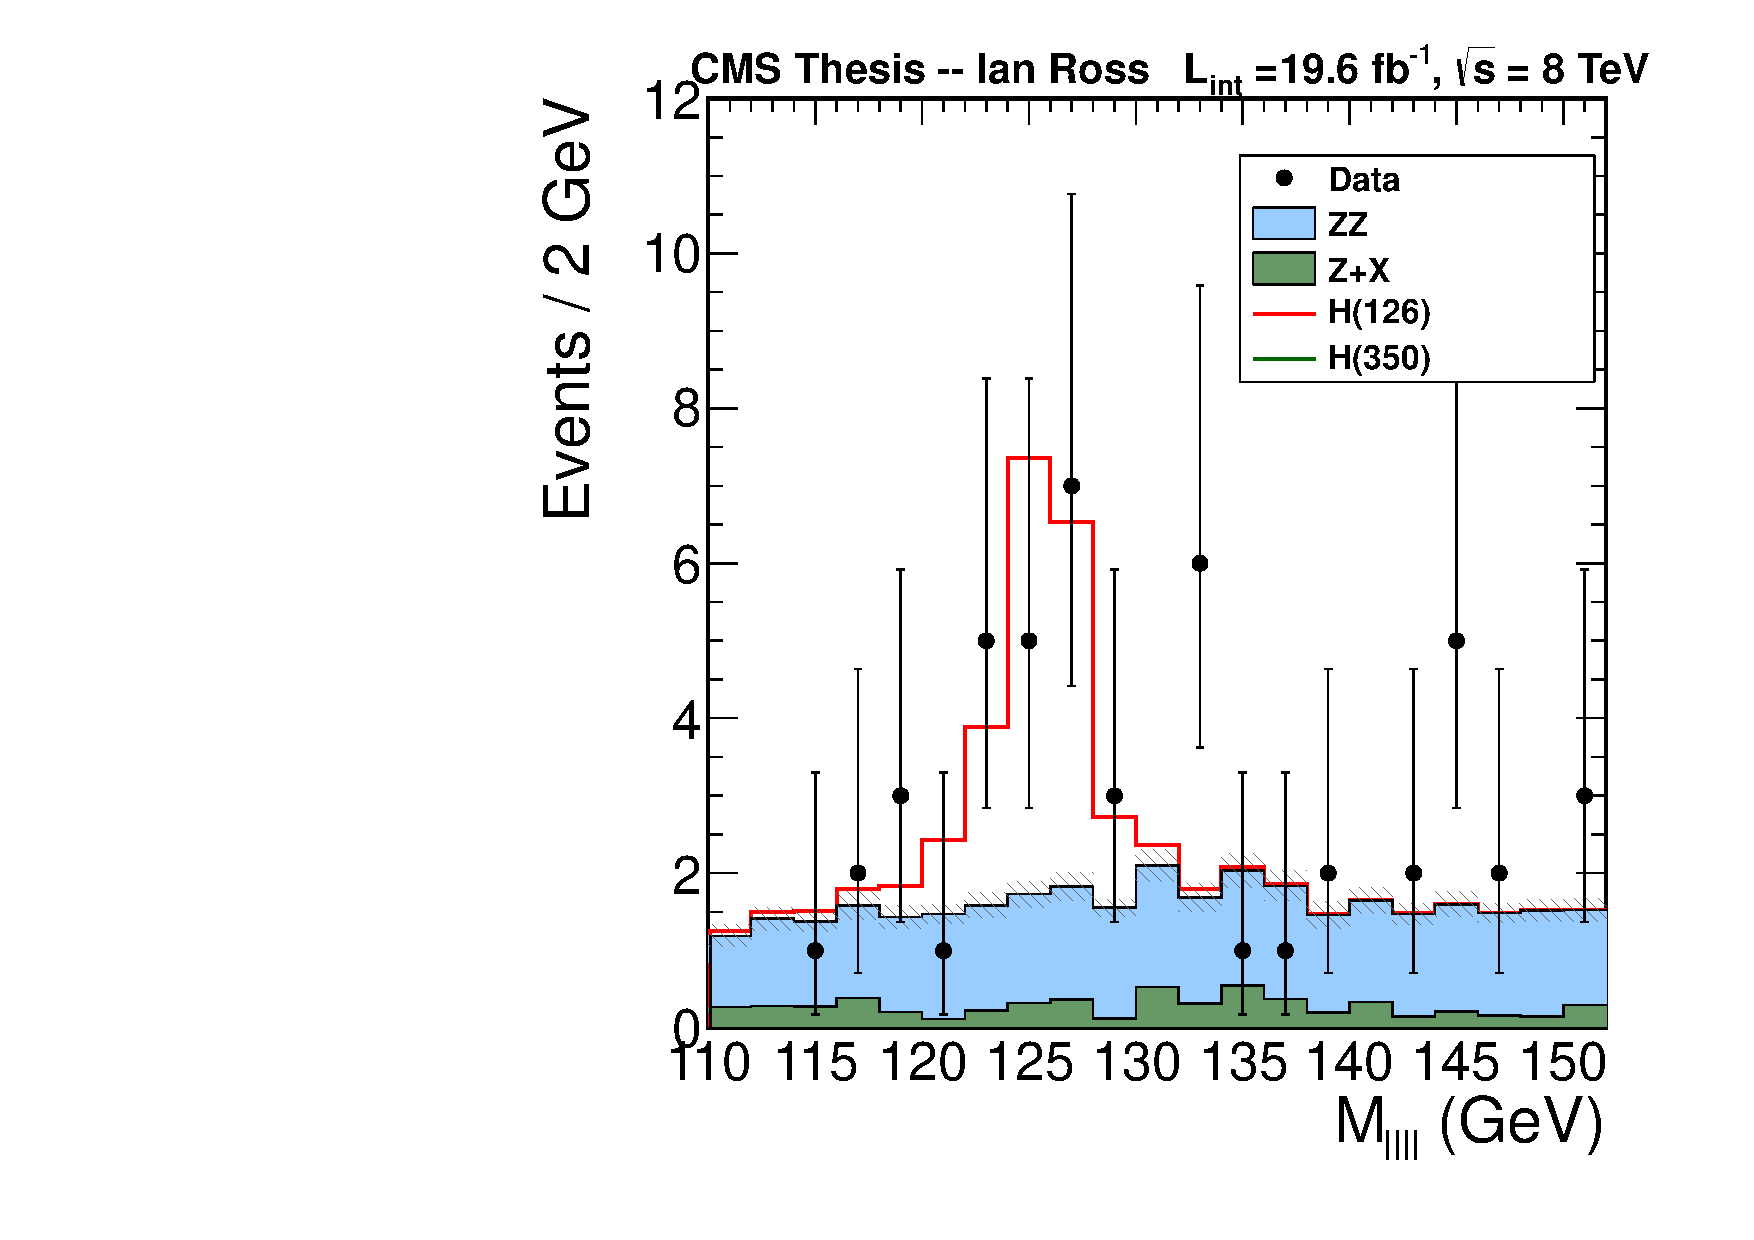
\includegraphics[width=0.40\textwidth]{4l_mass_low}
\caption[ZZ invariant mass including the low-mass $ZZ*$ analysis, zoomed to take a closer
look at the excess.]{ZZ invariant mass including the low-mass $ZZ*$ analysis, zoomed to take
a closer look at the excess. Pictured are
the eeee, $\mu\mu\mu\mu$, $\mu\mu e e$, and combined total results (upper left,
upper right, lower left, and lower right respectively).}
\label{fig:zzMass_higgs_low}
\end{figure}

\subsection{Statistical Analysis}
A test statistic, $q_\mu$, based on the likelihood function defined
in~\ref{eqn:likelihood}, is defined to extract upper limits:
\begin{equation}
    \tilde{q_\mu} = -2 \ln \frac{L (\mu, \vec{\theta_{s \mu}}, \vec{\theta_{b \mu}})}{L(\hat \mu,
    \hat{\vec{ \theta_{s}}}, \hat{\vec{ \theta_{b}}})}
\end{equation}
where $\hat \theta_{i \mu}$ are the conditional maximum likelihood estimators,
and $\hat \mu$, $\hat \theta_s$, and $\hat \theta_b$ are the parameters which
maximize the global likelihood.
From here, probability density functions are built for signal-plus-background
and background-only hypotheses. From these, p-values for the both scenarios are
calculated:
\begin{equation}
    p_\mu = P(\tilde{q_\mu} \ge \tilde{q_\mu^{obs}} |
    \textrm{signal+background})
\end{equation}
\begin{equation}
    1-p_b = P(\tilde{q_\mu} \ge \tilde{q_\mu^{obs}} |
    \textrm{background only})
\end{equation}
corresponding to the probability of observing a test statistic at least as large
as that observed, given a signal-plus-background or background only hypothesis.
Finally, the CLs value is defined to be the ratio between these probabilities:
\begin{equation}
    CLs = \frac{p_\mu}{1-p_b}
\end{equation}
The CLs value has the property that, given a value of $\mu$ and CLs value $\le
\alpha$, a Higgs of that signal strength is excluded at the $1-\alpha$
confidence level. Thus, to set a 95\% confidence level upper limit, the value of
$\mu$ is adjusted until the CLs value is 0.05.

Similarly, in order to find the significance of an observation, a test statistic
$q_0$ is defined:
\begin{equation}
    q_0 = -2 \ln \frac{L (0, \vec{\theta_{s 0}}, \vec{\theta_{b 0}})}{L(\hat \mu,
    \hat{\vec{ \theta_{s}}}, \hat{\vec{ \theta_{b}}})}
\end{equation}
Again, a pdf is constructed using pseudo-data and a background-only hypothesis,
and a p-value for the observed test statistic is constructed:
\begin{equation}
    p_\mu = P(q_0 \ge q_0^{obs})
\end{equation}
The corresponding significance of this p-value is taken from a normal one-sided
hypothesis scenario.  A full suite of tools has been developed in CMS to provide
the statistical framework for the search for the Higgs boson\cite{higgsStats}.

A local p-value scan is done across the full mass range, Figure~\ref{fig:pvals},
with a maximum local significance of $6.1\sigma$ observed at a Higgs mass of
126~GeV. 95\% confidence level upper limits are calculated from 110~GeV up to
1~TeV, excluding a Standard Model Higgs boson in the ranges of 130 to 600~GeV.   

\begin{figure}[h]
\centering
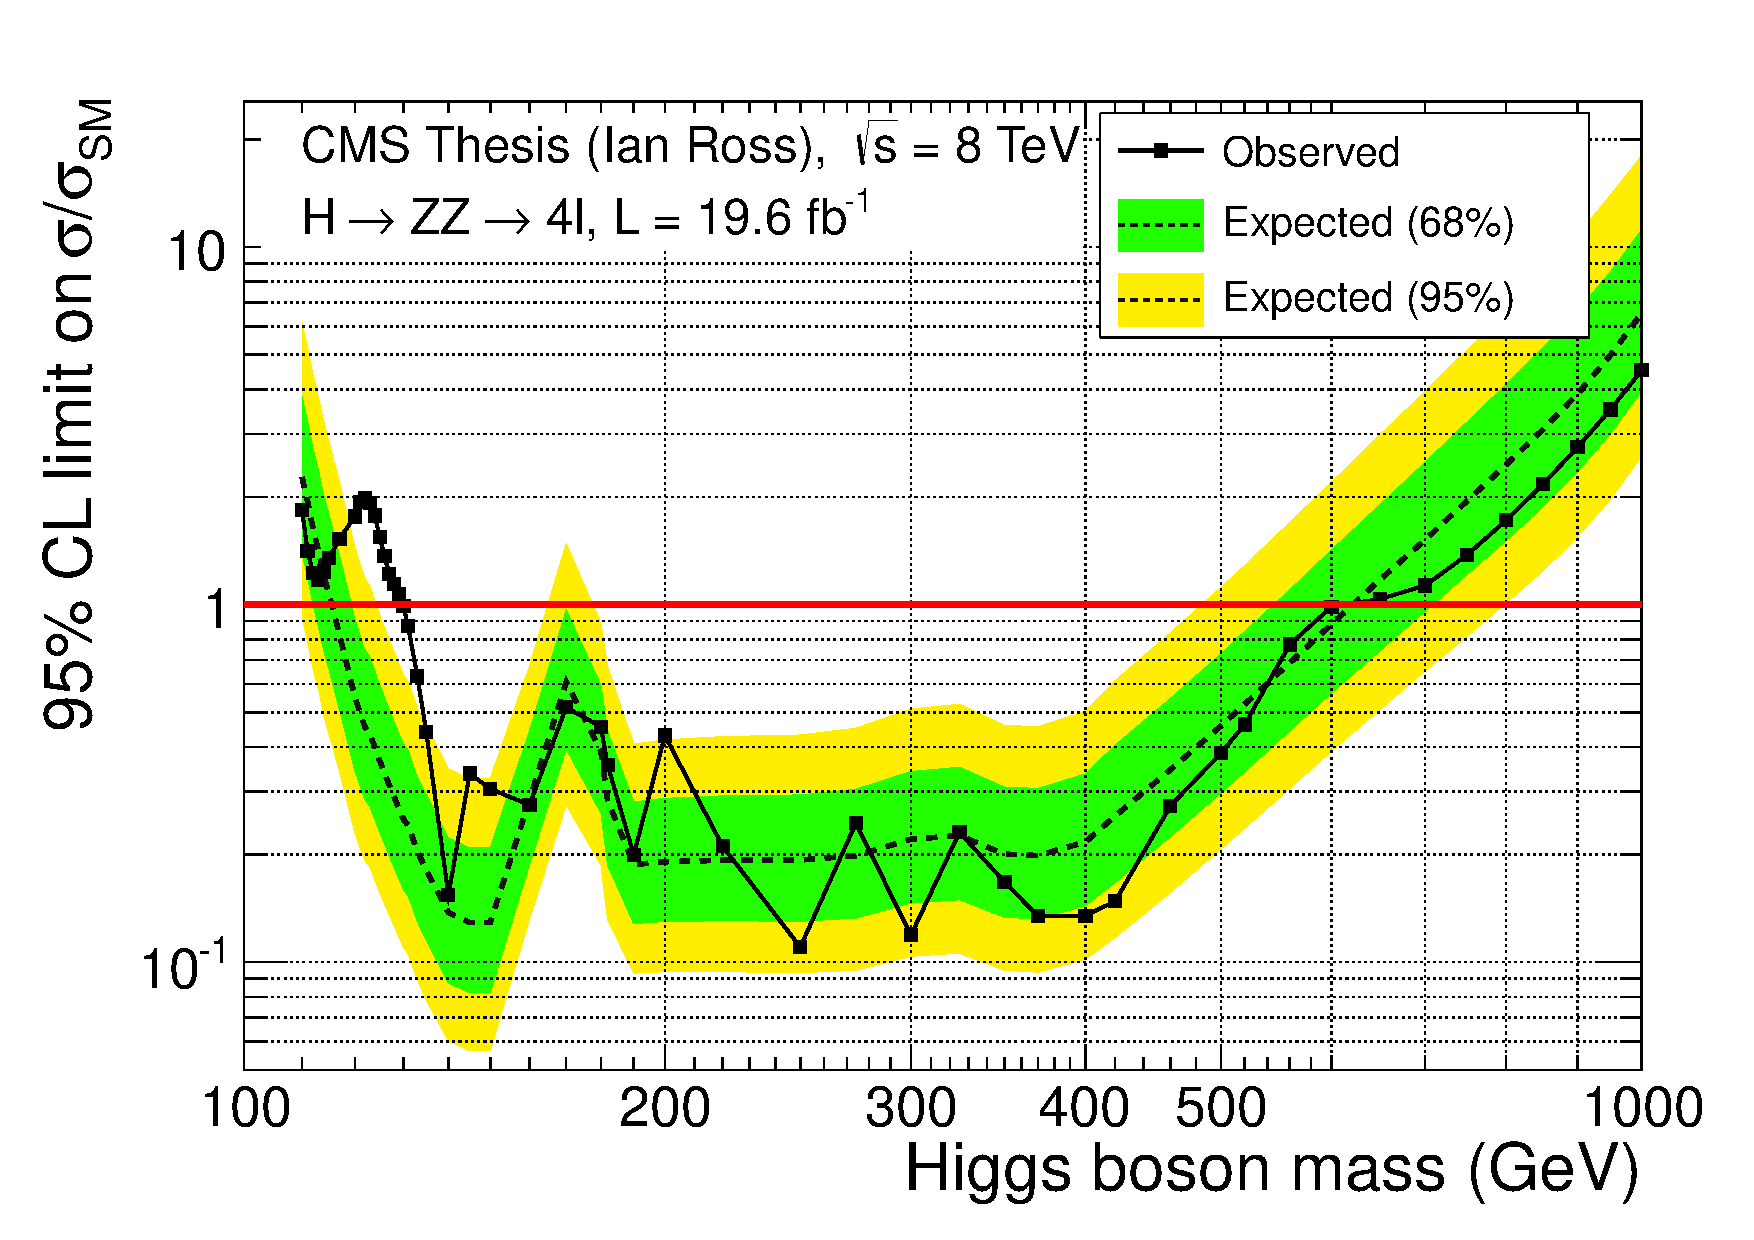
\includegraphics[width=0.45\textwidth]{higgs_limits_full}
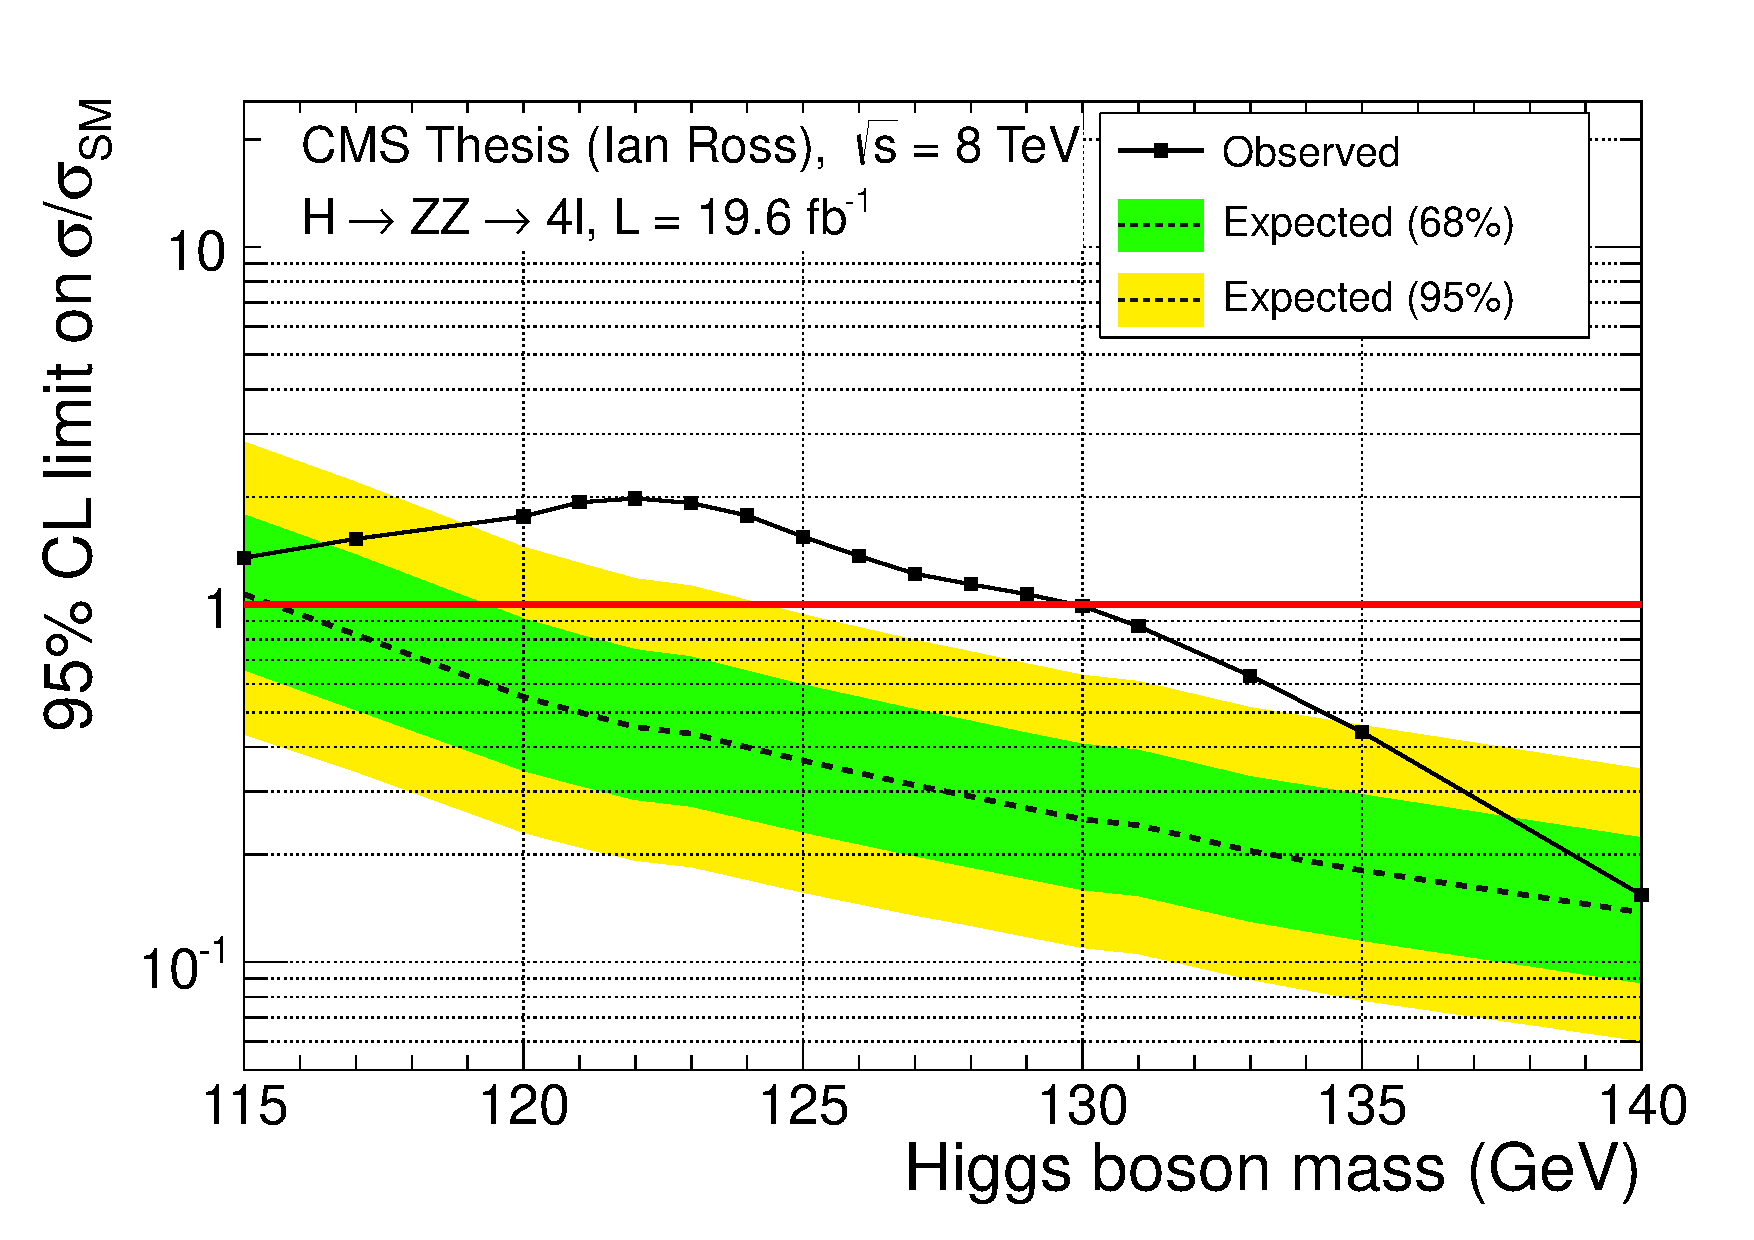
\includegraphics[width=0.45\textwidth]{higgs_limits_low} \\
\caption[95\% CL Upper Limits on Standard Model Higgs production.]{95\% CL Upper
Limits on Standard Model Higgs production (full mass range on the left, with a
low-mass scan on the right).}
\label{fig:higgsLimits}
\end{figure}

\begin{figure}[h]
\centering
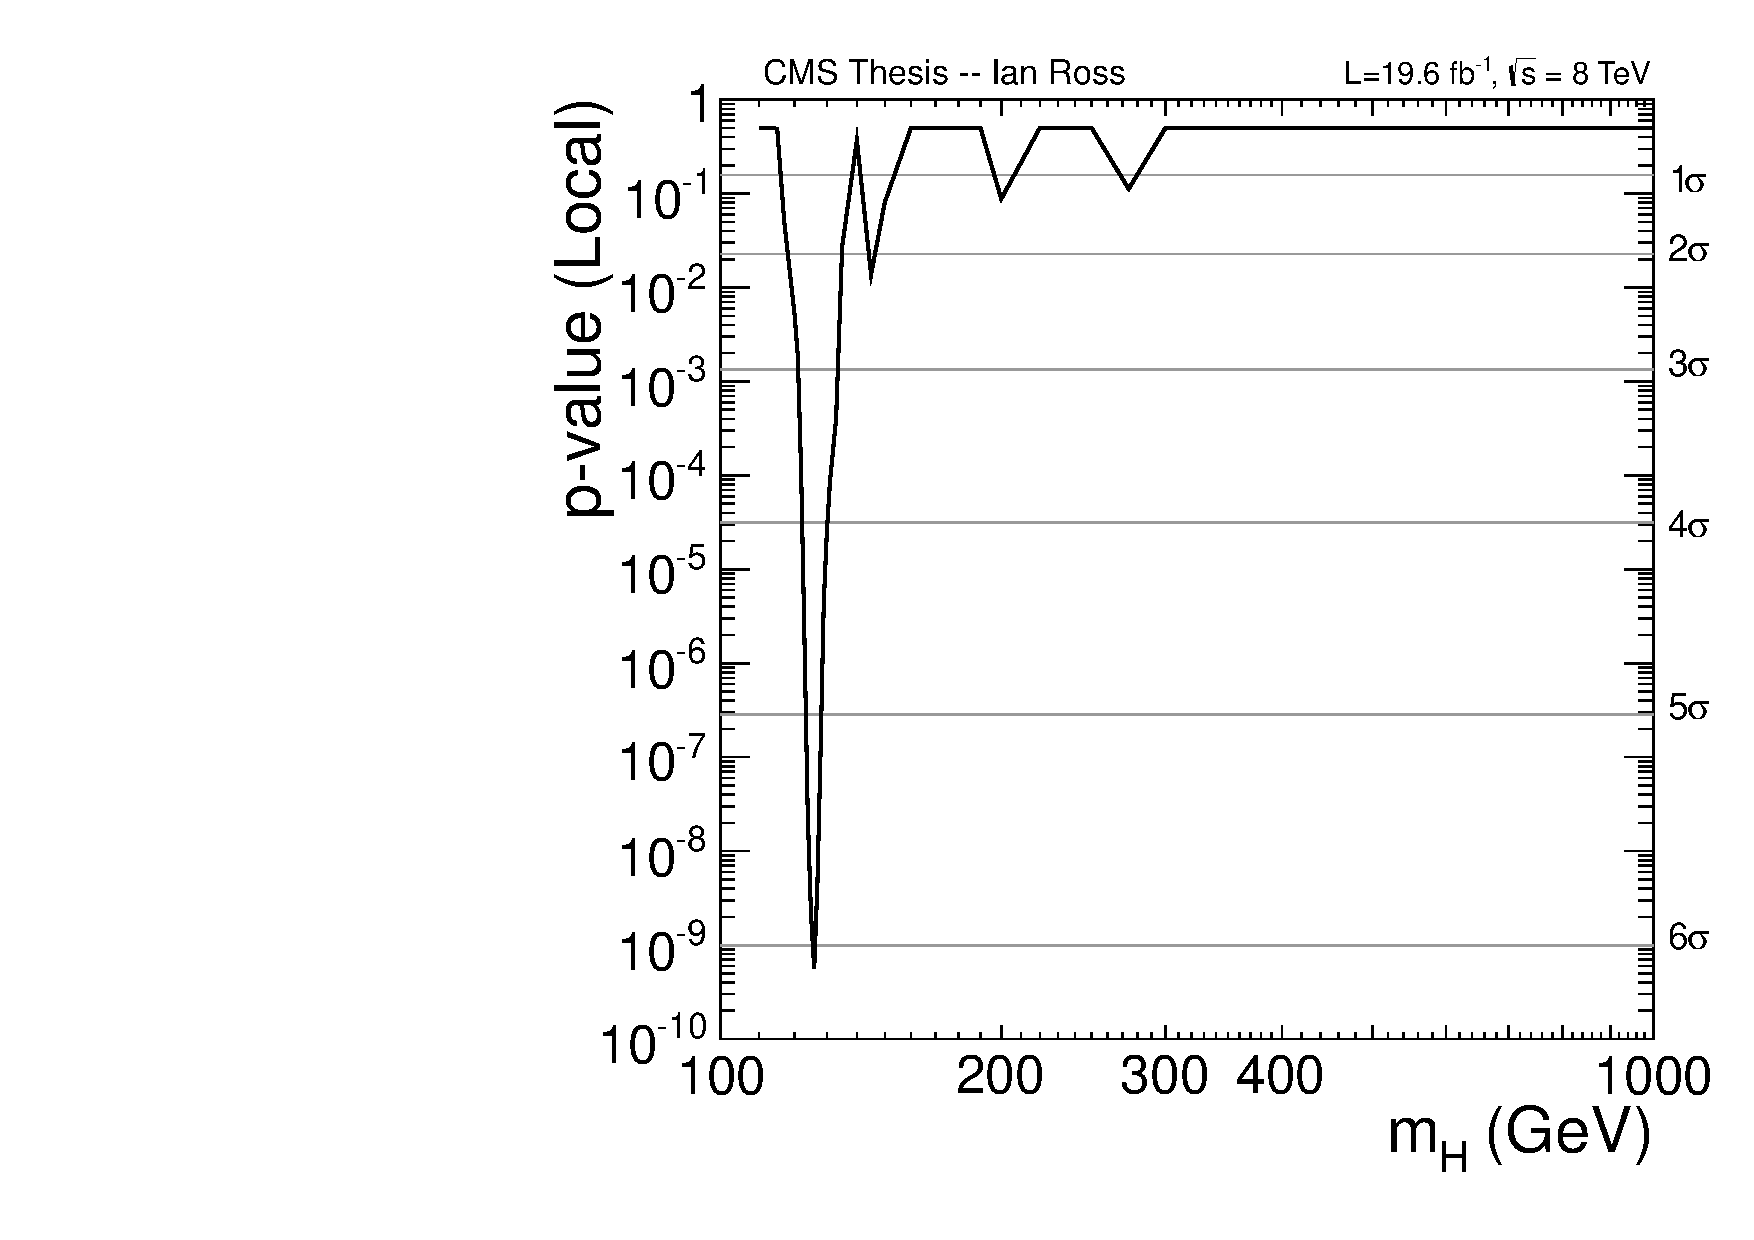
\includegraphics[width=0.45\textwidth]{pvals_full} 
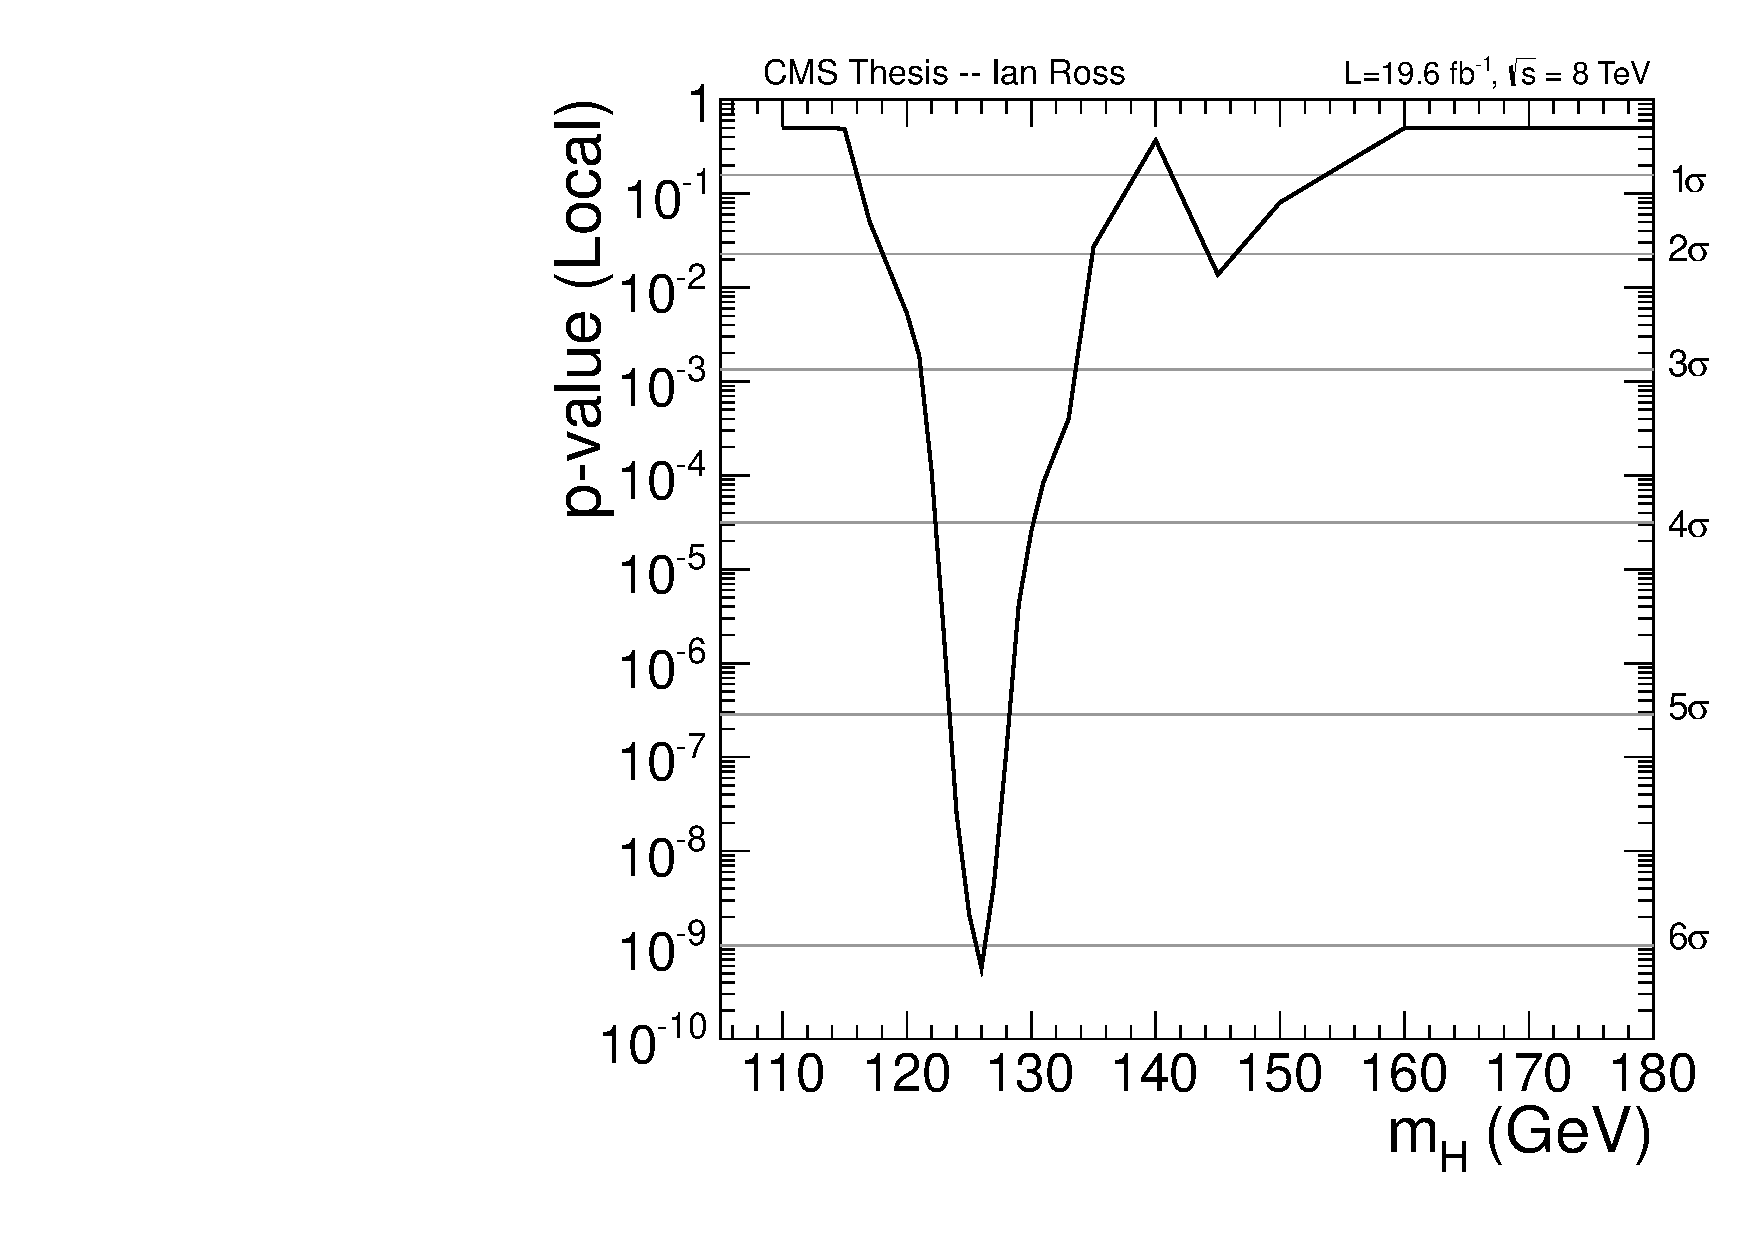
\includegraphics[width=0.45\textwidth]{pvals_low}\\
\caption[p-value scan.]{p-value scan for the full (left) and low (right) mass
ranges.}
\label{fig:pvals}
\end{figure}

\clearpage % get all the Higgs stuff dumped

\section{Limits on anomalous triple gauge couplings}
In order to set limits on the neutral triple gauge couplings, a binned counting
procedure is followed. First, a $3\times3$ grid of ($f_i^Z, f_i^\gamma$) Monte
Carlo simulations are generated in SHERPA~\cite{SHERPA} and fully simulated and
reconstructed. Because one of the major implications of the existence of
anomalous couplings is an enhanced high-mass tail in $M_{\ell \ell\ell\ell}$,
this variable is chosen as the discriminating variable. For each of the
generated samples, the $M_{\ell\ell\ell\ell}$ is plotted (using the same binning
for all samples). Yields in intermediary points in the coupling space are
interpolated bin-by-bin using a paraboloid fit to the existing samples, as
Fermi's Golden Rule suggests a quadratic dependence on cross section. A
likelihood for the null and alternative hypotheses is built, just like in the
Higgs case outlined above. However, in the case of the triple gauge coupling
limits, the CLs methodology is not used. Instead, a simple likelihood profiling
is used, using Wilks' theorem to set the confidence levels. The CLs limit %TODO:ref
procedure is not used because, by definition, it will never exclude the null
hypothesis. Given the presence of non-SM values of the couplings, the CLs limits
give limits which have little utility.

The invariant mass of the four-lepton system contains little information about
the sign of the couplings involved. The resulting likelihood scan shows this
degeneracy (Figure~\ref{fig:atgc_likelihood}), suggesting that only the size, but
not the sign, of the couplings could be extracted from this information.

\begin{figure}[h]
\centering
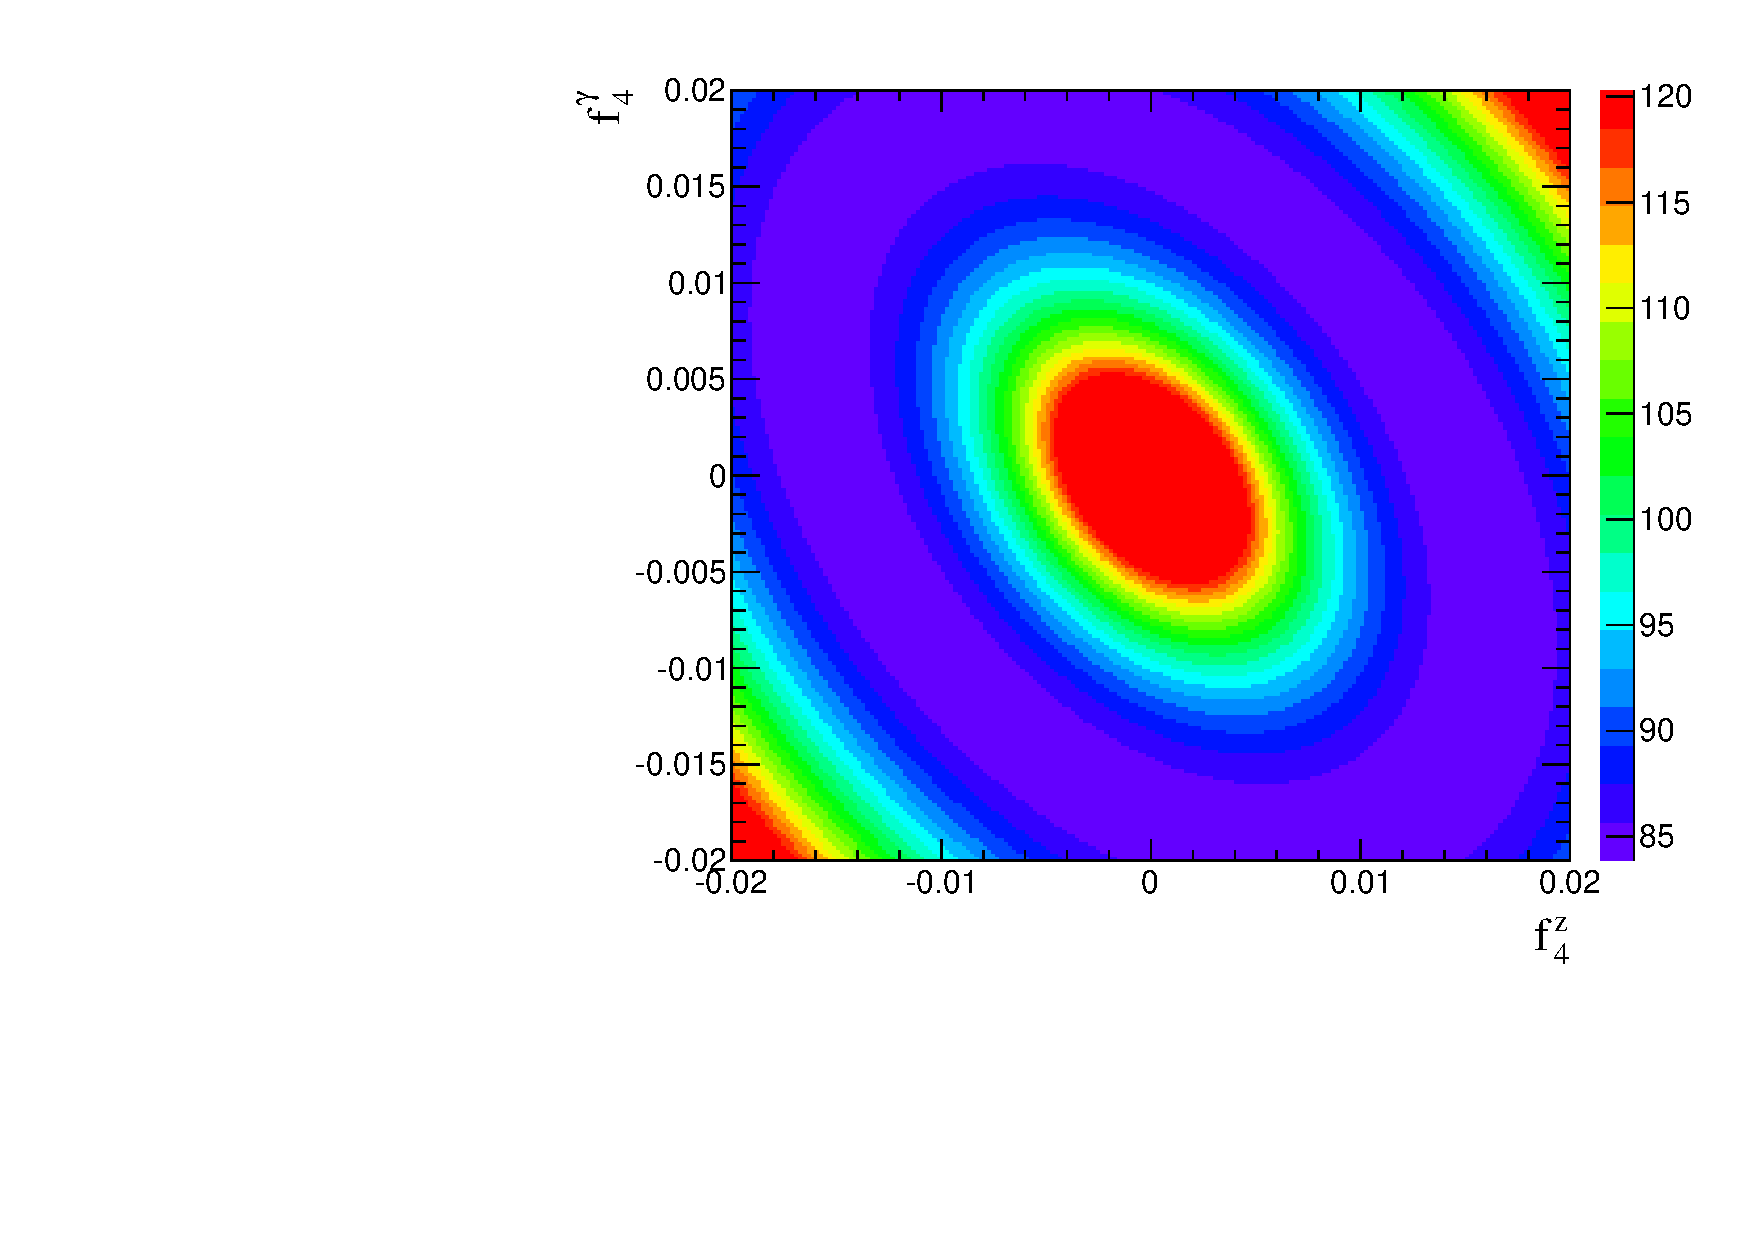
\includegraphics[width=0.80\textwidth]{contCanvas_fakeData.pdf}
\caption[Qualitative likelihood scan of the ($f_4^Z, f_4^{\gamma}$) coupling
space, with a signal injected.]{A qualitative
likelihood scan of the ($f_4^Z, f_4^\gamma$) coupling space, with an aTGC signal
injected. The degeneracy suggests that measurement of the sign of the couplings
would be impossible using just the information from the four-lepton invariant
mass.}
\label{fig:atgc_likelihood}
\end{figure}

Though SHERPA is a leading-order generator, it has been shown (see
Figure~\ref{fig:sherpaPowhegComp}) that SHERPA generation (with up to one extra
parton interaction) accurately reproduces the invariant mass kinematics of the
NLO POWHEG generation. This gives confidence that the differences between LO and
NLO in the discriminating variable ($M_{\ell\ell\ell\ell}$) are slight, and
SHERPA is an acceptable generator for the aTGC sample generation.

\begin{figure}[h]
\centering
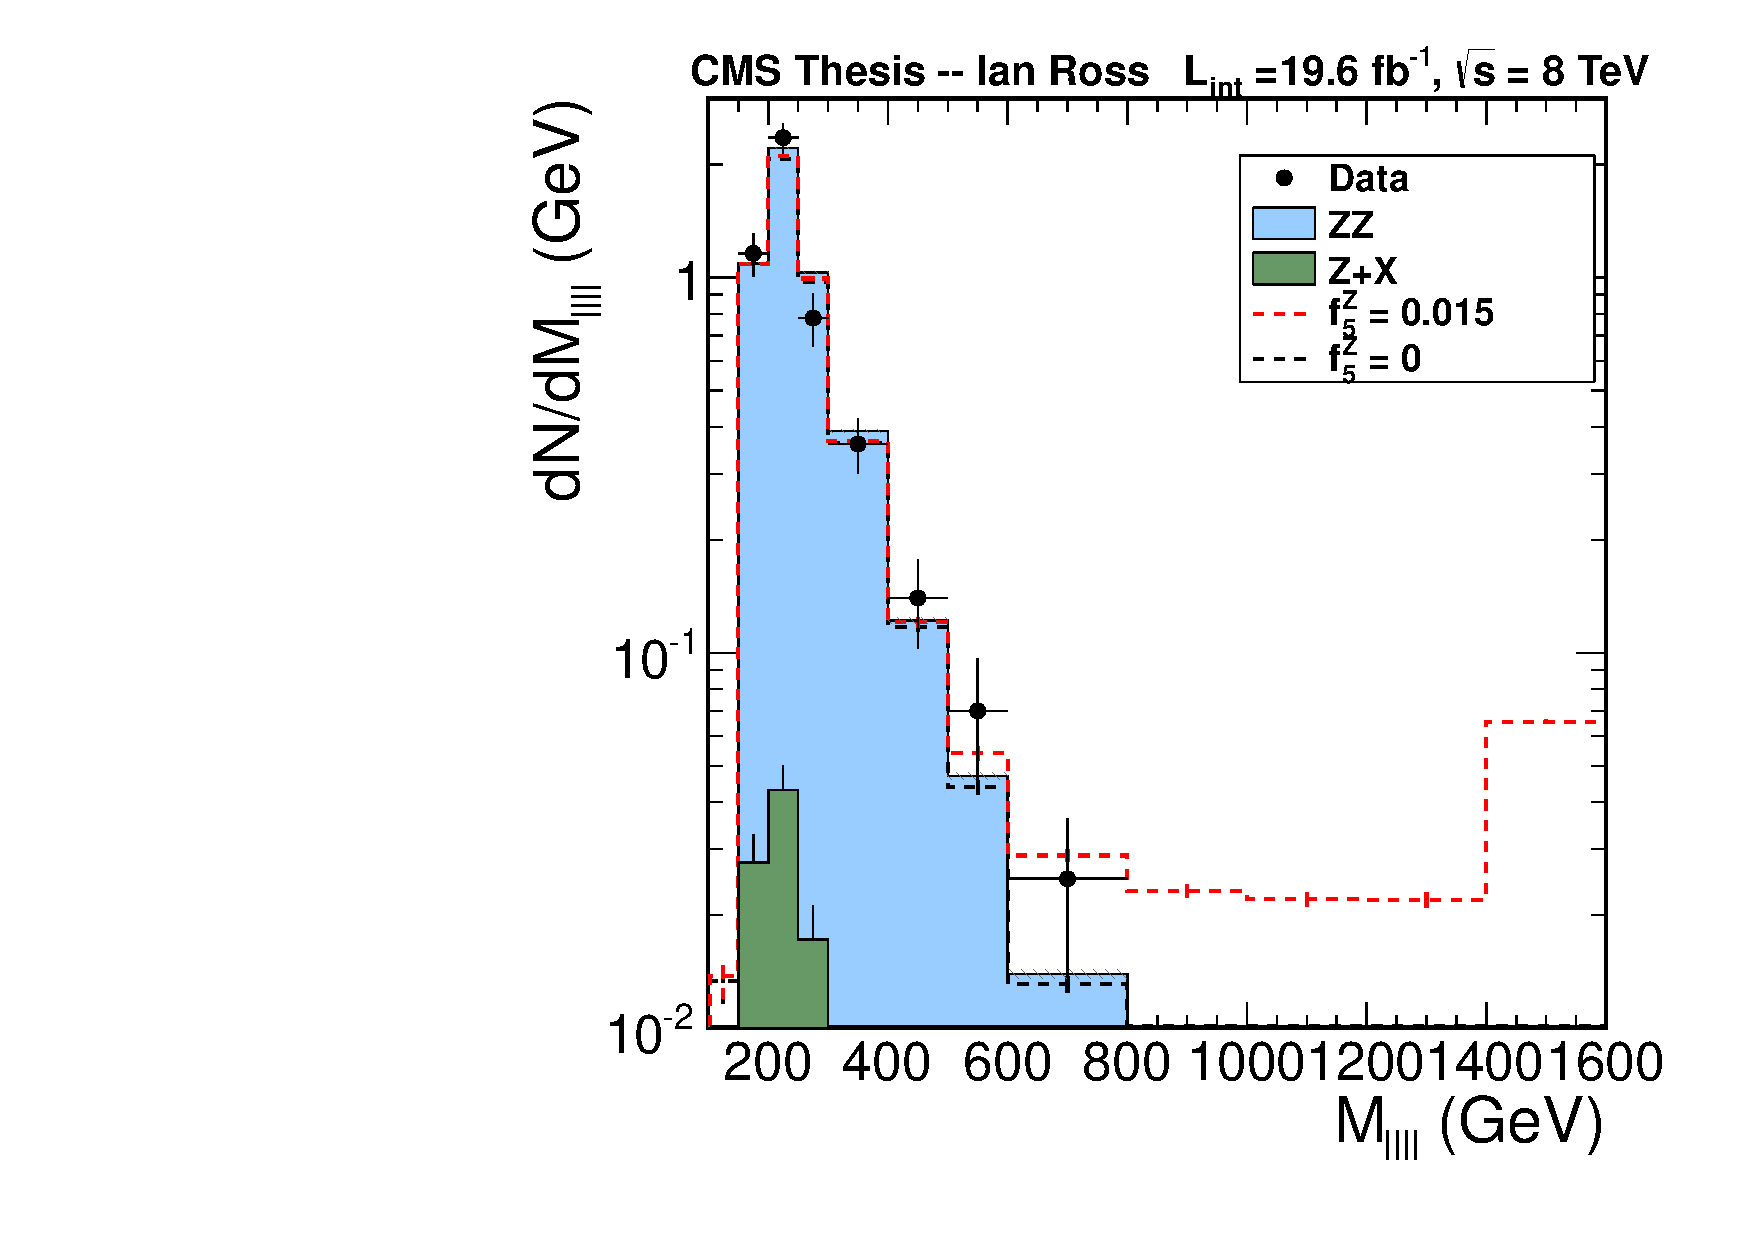
\includegraphics[width=0.80\textwidth]{sherpa_powheg_comp}
\caption[Comparison of the $M_{\ell\ell\ell\ell}$ for Standard Model ZZ production
by the LO generator SHERPA and the NLO POWHEG.]{Comparison of the
    $M_{\ell\ell\ell\ell}$ shape from Standard Model ZZ production by the LO generator
    SHERPA and the NLO POWHEG. Differences are slight, justifying the use of
SHERPA in generating the aTGC Monte Carlo samples. The last bin contains the
overflow of all higher $M_{\ell\ell\ell\ell}$ values.} 
\label{fig:sherpaPowhegComp}
\end{figure}

No significant deviation from the Standard Model expectations are observed, and
95\% Confidence Level upper limits are set using profile likelihood methodology.
Limits are extracted for the two dimension $(f_4^Z, f_4^{\gamma})$ and $(f_5^Z,
f_5^{\gamma})$ coupling spaces separately (with the other two couplings held to
0). Additionally, single-coupling limits are calculated by restricting the other
couplings to 0. The two- and one-dimensional limits are depicted in
Figure~\ref{fig:atgc_limits}, and the one-dimensional limits are presented in
Table~\ref{tab:atgc_limits}.

\begin{figure}[h]
\centering
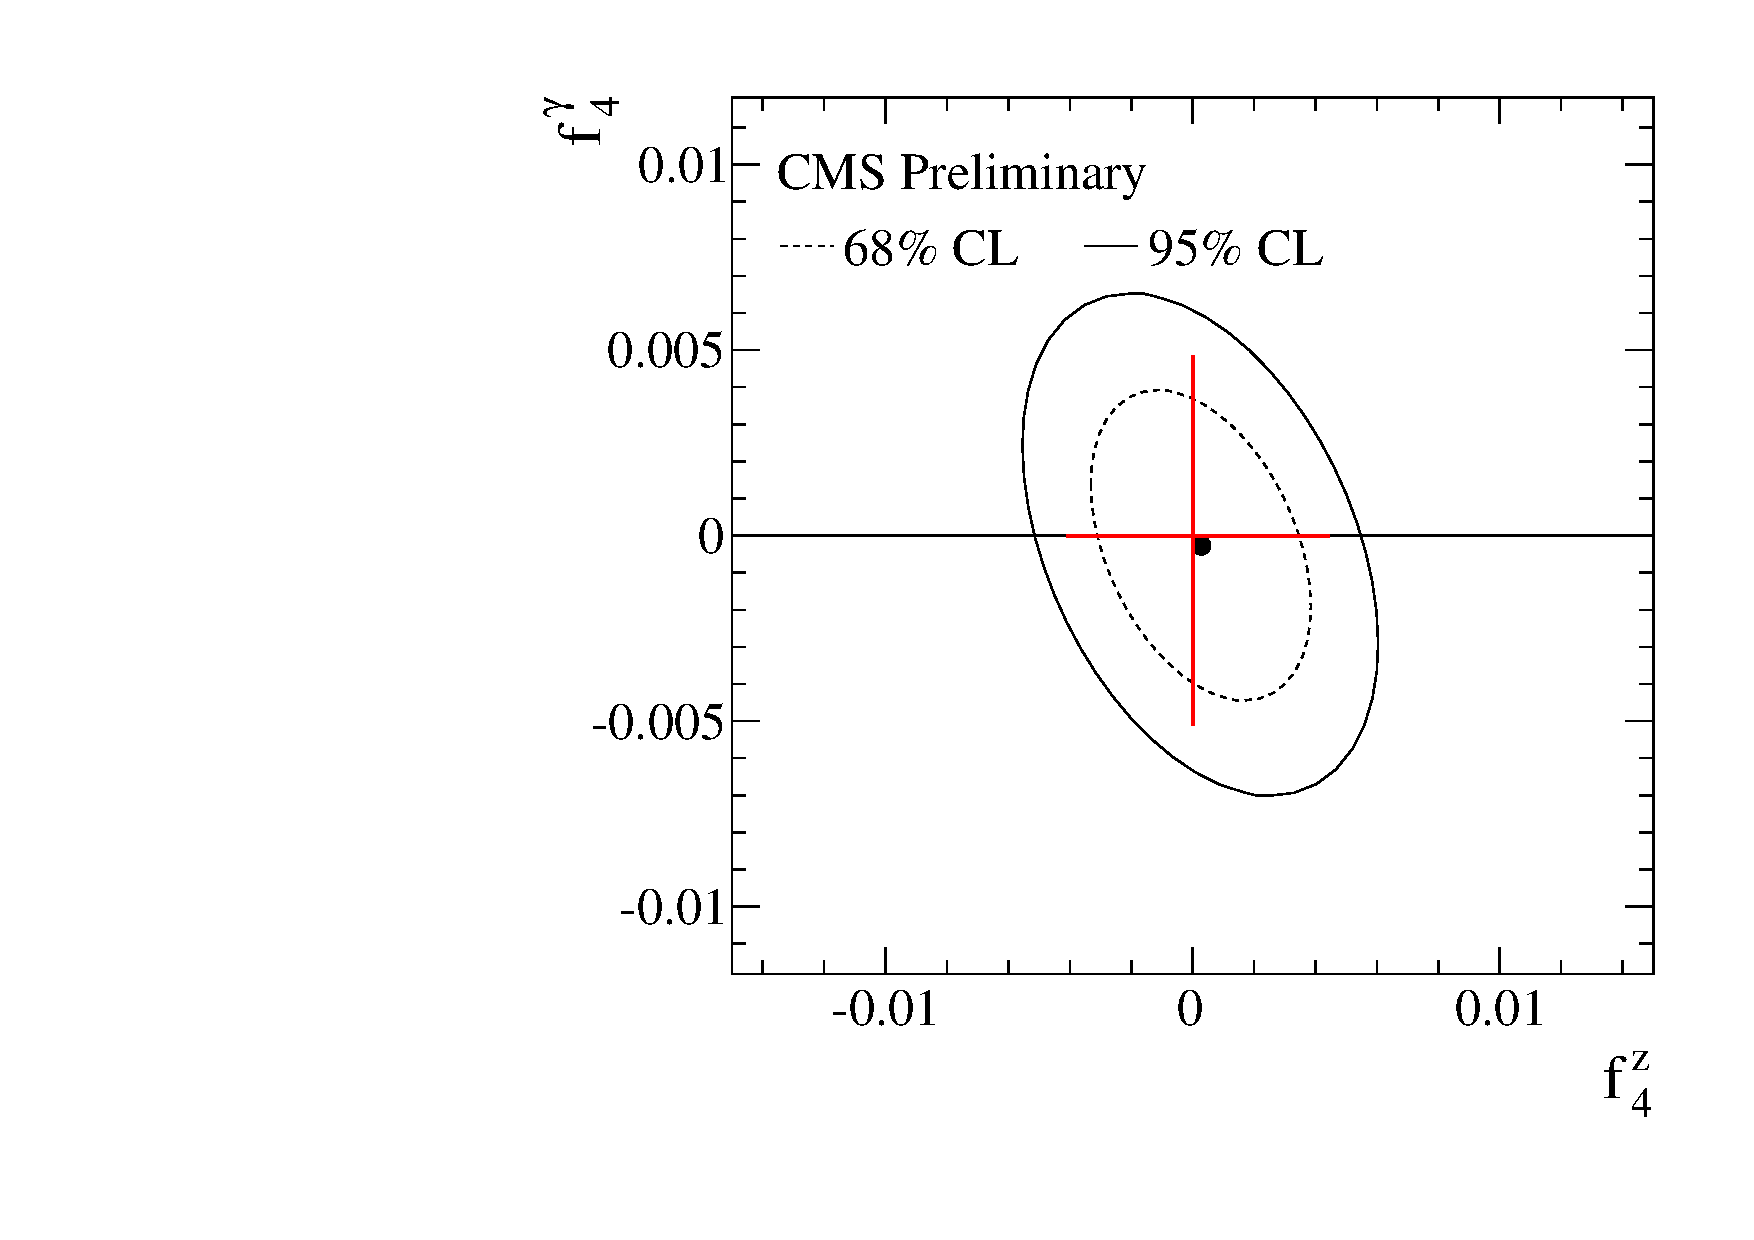
\includegraphics[width=0.45\textwidth]{lim_f4z_f4g}
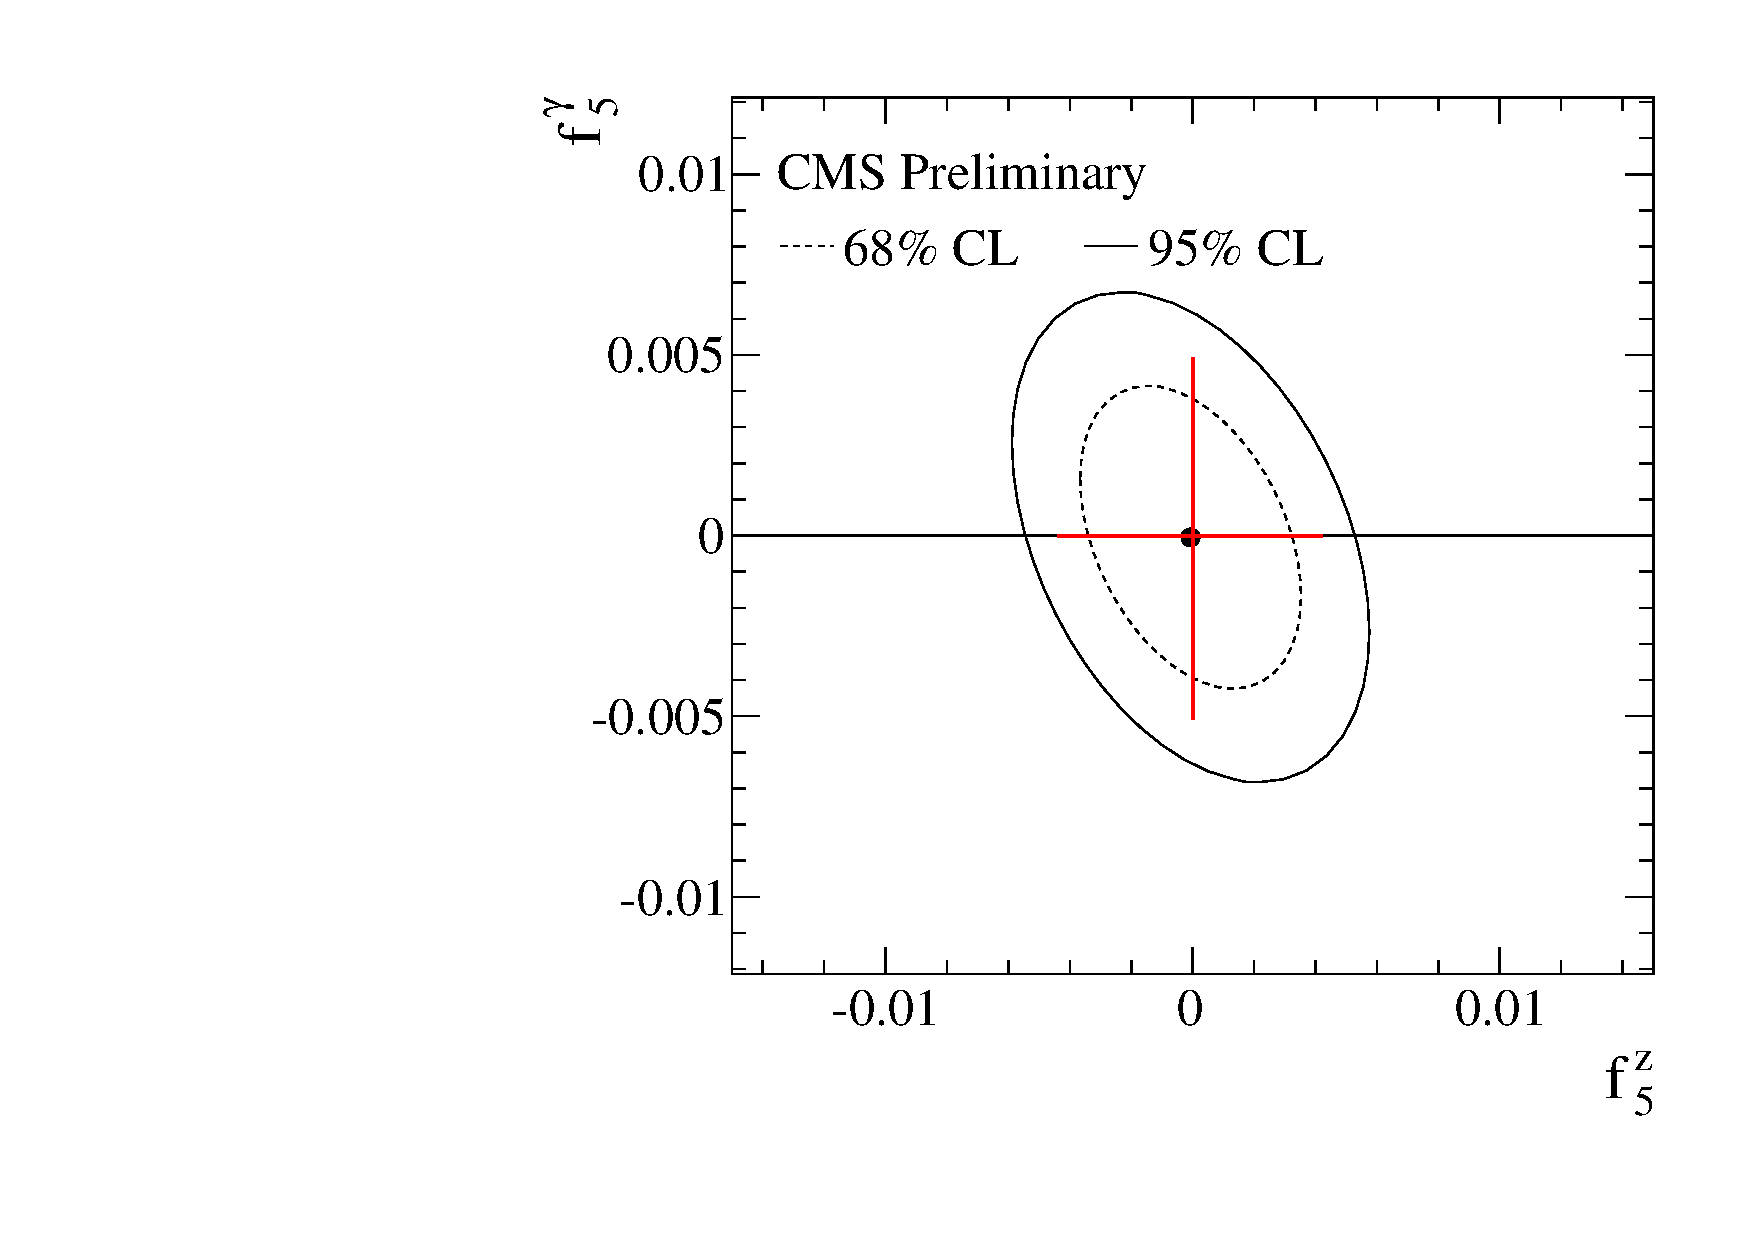
\includegraphics[width=0.45\textwidth]{lim_f5z_f5g}
\caption[2D limits on the neutral anomalous triple gauge couplings.]{2D limits
on the neutral anomalous triple gauge couplings. The solid line represents the 95\%
confidence level on the 2D coupling, the dashed line represents the 68\%
confidence level, and the red lines represent the 95\% confidence level
limits (with the other couplings constrained to 0). The block dot represents the
best-fit coupling values.}
\label{fig:atgc_limits}
\end{figure}

\begin{table}[h]
\centering
\begin{tabular}{|c|c|c|}
    \hline
i  & $f_{i}^Z $& $f_{i}^{\gamma} $ \\
\hline
$4$ & $-0.004 < f_4^Z < 0.004 $&$ -0.005 < f_4^{\gamma} < 0.005 $\\
$5$ & $-0.004 < f_5^Z < 0.004 $&$ -0.005 < f_5^{\gamma} < 0.005 $\\
\hline
\end{tabular}
\caption[1D limits on the neutral anomalous triple gauge couplings.]{1D limits
on the neutral anomalous triple gauge couplings. Values are extracted by holding
the other three neutral couplings to 0.}
\label{tab:atgc_limits}
\end{table}
\clearpage

